\documentclass[tcc,capa]{texufpel}

\usepackage[utf8]{inputenc} % acentuacao
\usepackage{graphicx} % para inserir figuras
\usepackage[T1]{fontenc}
\usepackage{comment}
\usepackage{amsfonts}
\usepackage{todonotes}
\usepackage{lscape}
\usepackage{threeparttable}
\usepackage{colortbl}
\usepackage{scalefnt}
\usepackage{graphics}
\usepackage{graphicx}
%\usepackage[small,bf]{caption}https://www.overleaf.com/3183347328wjggqqvdkthm
\usepackage{amssymb}
\usepackage{subfigure}
\usepackage{float}
\usepackage{subfloat}
\usepackage{multirow}
%\usepackage{multicolumm}
\usepackage{xcolor}
\usepackage{pdfpages}
\usepackage{amsmath}
\usepackage{amssymb}

%\newcommand {\BM} {\todo[inline, color=green!40]}
%\usepackage[color=yellow!40]{todonotes}
\newcommand{\BM}[2][]{\todo[color=green, size=\footnotesize #1]{#2}}
%\usepackage[normalem]{ulem} 

\newcommand{\mlp}[1]{\todo[color=red]{#1}}
\newtheorem{Def}{Defini\c c\~ao}

\hypersetup{
    hidelinks, % Remove coloração e caixas
    unicode=true,   %Permite acentuação no bookmark
    linktoc=all %Habilita link no nome e página do sumário
}

\unidade{Centro de Desenvolvimento Tecnológico}
\curso{Ciência da Computação}
\nomecurso{Bacharelado em Ciência da Computação}
\titulocurso{Bacharel em Ciência da Computação}

\title{f-ClouD: Sistema Fuzzy para Avaliação da Utilização de Servidores em um Ambiente Simulado de Computação em Nuvem}

%% Alguns possíveis títulos

%f-ClouD: Abordagem Fuzzy Tipo-2 para Detecção da Sobrecarga de Hosts para Ambiente de Computação em Nuvem

%f-ClouD: Abordagem Fuzzy Tipo-2 para Gerência de Recursos em um Ambiente Simulado de Computação em Nuvem

%Int-fCloud?


\author{Schneider}{Guilherme Bayer}
\advisor[Profa.~Dr.]{Reiser}{Renata Hax Sander}
\coadvisor[Prof.~Dr.]{Yamin}{Adenauer Corrêa}
\collaborator[Ms.]{Moura}{Bruno Moura Paz de}

%Palavras-chave em PT_BR
\keyword{Lógica Fuzzy tipo-2}
\keyword{Computação em Nuvem}
\keyword{Computação Ecológica}
\keyword{Alocação de Máquinas Virtuais}

%Palavras-chave em EN_US
\keywordeng{Type-2 Fuzzy Logic}
\keywordeng{Cloud Computing}
\keywordeng{Green Computing}
\keywordeng{Virtual Machine Allocation}

\begin{document}

\renewcommand{\advisorname}{Orientadora}           %descomente caso tenhas orientadora
%\renewcommand{\coadvisorname}{Coorientadora}      %descomente caso tenhas coorientadora

\maketitle 

\sloppy

\fichacatalografica

\folhadeaprovacao

%Opcional
\begin{dedicatoria}
  Dedico este trabalho principalmente minha família que me apoiou incondicionalmente em todo o desenvolvimento e também aos meus colegas que me auxiliaram em toda minha trajetória.
\end{dedicatoria}

%Opcional
\begin{agradecimentos}
  A todos os professores, em especial a Renata, pela orientação e apoio durante o curso e no desenvolvimento deste trabalho.
  
  A todos os amigos do curso, com quais pude compartilhar momentos e experiências da graduação.
  
  A minha família por me acompanharem nesse processo e estarem sempre à disposição quando eu precisei.
\end{agradecimentos}

%Opcional
%\begin{epigrafe}
%  {\sc --- Fulano de Tal}
%\end{epigrafe}

%Resumo em Portugues (no maximo 500 palavras)
\begin{abstract}
  A consolidação dinâmica de máquinas virtuais (MVs) é uma maneira eficaz de melhorar a utilização de recursos e a eficiência energética na Computação em Nuvem (CN). Determinar quando é melhor realocar MVs de um host sobrecarregado é um aspecto dinâmico da consolidação de MVs que influencia diretamente na utilização de recursos e na qualidade de serviço oferecida pelo provedor. Este trabalho apresenta uma nova proposta com uma abordagem de Lógica Fuzzy Tipo-2 para tratar as incertezas e imprecisões quanto da determinação do uso de recursos no ambiente de CN, visando economia energética com degradação mínima de desempenho. Resultados são obtidos em um ambiente simulado, e mostram melhorias na eficiência energética alcançando valores de 15,64\% no emprego com o algoritmo \textit{Median Absolute Deviation} (MAD), 15,43\% no caso do \textit{Inter Quartile Range} (IQR) e 9,19\% com \textit{Local Regression} (LR).
\end{abstract}

\begin{englishabstract}%
  {f-Cloud: Fuzzy System for Evaluating Server Usage in a Simulated Cloud Computing Environment}
  
  The dynamic consolidation of virtual machines (VMs) is an effective way to improve resource utilization and energy efficiency in cloud computing. Determining when it is best to relocate VMs from an overloaded host is a dynamic aspect of VM consolidation that directly influences resource utilization and Quality of Service (QoS) offered by the system. This paper presents a new proposal with a Fuzzy Type-2 Logic approach to address the uncertainties and inaccuracies of determining resource usage in the cloud computing environment, thereby aiming at energy savings with minimal performance degradation. Results are obtained in a simulated cloud computing environment, and show improvements in energy efficiency reaching 15.64\% in employment with the Median Absolute Deviation (MAD), 15.43\% in the case of the Inter Quartile Range (IQR) and 9.19\% with Local Regression (LR).
  
\end{englishabstract}

%Lista de Figuras
\listoffigures

%Lista de Tabelas
\listoftables

%lista de abreviaturas e siglas
\begin{listofabbrv}{SPMD}
        \item[LC] Lógica Clássica
        \item[LF] Lógica Fuzzy
        \item[SF] Sistema Fuzzy
        \item[CF] Conjunto Fuzzy
        \item[TI] Tecnologia da Informação
        \item [LF1] Lógica Fuzzy Tipo-1
        \item [LF2] Lógica Fuzzy Tipo-2
        \item[CN] Computação em Nuvem
        \item[MF] Máquina Física
        \item[MV] Máquina Virtual
        \item[QoS] \textit{Qualidade of Service}
        \item[SLA] \textit{Service Level Agreements}
        \item[SLO] \textit{Service Level Object}
        \item[TCF] Teoria dos Conjuntos Fuzzy
        \item[IVFL] Lógica fuzzy valorada intervalarmente
        \item[T1FS] \textit{Type-1 Fuzzy System}
        \item[T2FS] \textit{Type-2 Fuzzy System}
        \item[SBRF1] Sistema Baseado em Regras Fuzzy Tipo 1
        \item[SBRF2] Sistema Baseado em Regras Fuzzy Tipo 2
        \item [BR] Base de Regras
        %\item[UFPEL] Universidade Federal de Pelotas
\end{listofabbrv}

%Sumario
\tableofcontents

\chapter{Introdução} \label{capIntroducao}

A Computação em Nuvem (CN) é um paradigma computacional constituído das categorias de Infraestrutura (IaaS), Plataforma (PaaS) e Software (SaaS) como Serviço usando um modelo de pagamento por uso. Na CN \textit{data centers} são usados para hospedagem das aplicações e conhecidos por demandar grande quantidade de eletricidade, elevando o custo operacional para os provedores e contribuindo com a emissão de CO2 no meio ambiente \cite{ToosiAndBuyya2015}. A principal vantagem deste paradigma é que ambos clientes e provedores podem ajustar rápida e continuamente a alocação de recursos com base nas necessidades atuais, característica conhecida como elasticidade \cite{mell2011nist}.

De acordo com o relatório do Conselho de Defesa dos Recursos Naturais (NRDC)\footnote{https://www.nrdc.org/} dos Estados Unidos (EUA), em 2014, somente os seus data centers consumiram uma estimativa de 70 bilhões de quilowatts/hora (kWh), representando cerca de 1,8\% do seu consumo total de eletricidade~\cite{shehabi2016united}.

A busca por eficiência energética sem perda de desempenho fez com que diversos conceitos fossem propostos, com destaque na CN, consistindo em uma distribuição dos serviços de computação (alocação de servidores, armazenamento, banco de dados, etc) em que não há a necessidade do usuário fazer grande investimento em equipamentos, e ainda, com pagamento associado ao tempo de uso \cite{nathani2012policy}.

O problema de minimização do consumo energético na CN considerando restrições referentes a qualidade de serviços (\textit{Quality of Service} - QoS) é analiticamente complexo, e demanda investimentos na consolidação dinâmica de Máquinas Virtuais (MVs), que é um problema NP-Difícil \cite{HiltunenEtAl2010, BeloglazovAndBuyya2013}.

Neste contexto, os principais desafios da CN são: (i) provisionamento automático de serviço; (ii) migração de MVs; (iii) consolidação de servidores, (iv) gerenciamento de energia, e ainda, (v) segurança de dados. Este trabalho contempla a migração e consolidação de MVs com uma abordagem para utilização eficiente dos servidores físicos do ambiente da CN e buscando, simultaneamente manter um padrão satisfatório de \textit{Qualidade de serviço} (QoS)  e \textit{Service Level Agreements} (SLA).

Na concepção da abordagem proposta, foi utilizado o formalismo matemático e a fundamentação da Lógica Fuzzy (LF). A LF, lógica nebulosa, ou ainda, lógica difusa, é uma lógica multivalorada capaz de absorver informações vagas, normalmente descritas em uma linguagem natural e convertê-las para um formato numérico de fácil manipulação computacional. Esta facilidade se mostra oportuna para o uso na etapa de consolidação de MVs, procurando com isso modelar os modos imprecisos do raciocínio na tomada de decisões a partir de informações obtidas através da infraestrutura computacional.

\section{Objetivos}

O objetivo deste trabalho é o desenvolvimento do \emph{fClouD}: Um módulo para tomada de decisões empregando abordagem da Lógica Fuzzy Tipo-2 capaz de tratar a incerteza do especialista em determinar a utilização de uma máquina física no ambiente de CN, considerando desde sua modelagem até a prototipação e validação.

O trabalho considera como estratégia a integração da CN com a LF, objetivando filtrar as principais métricas disponíveis no ambiente e, assim propor a modelagem e consolidar a implementação do componente \emph{f-ClouD}, incluindo a posterior prototipação, e considerando a análise de desempenho dos resultados gerados.

Considerando este objetivo geral, os objetivos específicos elencados são:

\begin{enumerate}
    %\item Estudo das fundamentações na concepção da CN;
    \item Estudo das fundamentações da CN;
    \item Estudo das fundamentações da LF;
    \item Estudo do Int-fGrid~\cite{moura2018int} para fundamentação do f-ClouD;
    %\item Desenvolvimento e prototipação do componente f-ClouD considerando o ambiente de CN determinado via simulador estendendo o Int-fGrid~\cite{moura2018int};
    \item Desenvolvimento e prototipação do componente \emph{f-ClouD} estendendo o Int-fGrid~\cite{moura2018int};
    \item Integração do módulo \emph{f-ClouD} com simulador de CN;
    \item Validação do componente \emph{f-ClouD}, comparando com algoritmos clássicos utilizados na CN.
\end{enumerate}

\section{Estrutura do trabalho}

Este trabalho está estruturado da seguinte forma: no Capítulo \ref{capIntroducao}, está a introdução e os objetivos. No Capítulo \ref{sec:computacaoemnuvem}, tem-se a fundamentação da CN. No Capítulo \ref{sec:fuzzy} apresenta a fundamentação da LF. No Capítulo \ref{sec:modelagem}, são apresentados os principais aspectos para a concepção, modelagem e prototipação dos sistemas fuzzy propostos para auxiliar na tomada de decisão. Logo a seguir, no Capítulo \ref{capAnaliseDeDesempenho}, são apresentados os resultados obtidos. E, por fim, no Capítulo \ref{capConclusao} consta as principais conclusões.



\chapter{Computação em Nuvem} \label{sec:computacaoemnuvem} 

Com o rápido desenvolvimento das tecnologias de processamento e armazenamento juntamente com a busca por maximizar o consumo energético intensificam-se a pesquisa por novas alternativas frente aos paradigmas antigos de computação. Neste contexto, surge o modelo computacional denominado CN, no qual recursos são disponibilizados de acordo com o tempo de usabilidade. Sendo assim, tem-se a possibilidade de haver uma cobrança mais flexível, como por exemplo, um determinado servidor ser utilizado por um determinado número de horas sendo cobrado só por aquele tempo e não por uma mensalidade. 

Apesar do atual destaque dado a pesquisa em CN, seu conceito não é novo e tão pouco suas tecnologias \cite{hamdaqa2012cloud}. Em 1960, John McCarthy acreditava que um dia corporações conseguiriam vender recursos computacionais como “commodity” \cite{holick2011evaluation}.

O surgimento da CN causou um grande impacto nas industrias de tecnologia de informação, sendo elas Google, Amazon e Microsoft que constantemente batalham para terem um ambiente de CN mais potente, confiável e eficiente energeticamente.

O objetivo deste capítulo é apresentar um estudo sobre a CN, suas características, definições, desafios e simuladores.


%O objetivo deste capítulo é apresentar um estudo sobre a Computação em Nuvem, suas características, definições, desafios e arquitetura.


\section{Definição}

A NIST (National Institute of Standards and Technology) em “The NIST Definition of Cloud Computing” \cite{mell2011nist} define a CN nos termos abaixo:

\begin{comment}
“Cloud Computing is a model for enabling ubiquitous, convenient, ondemand network access to a shared pool of configurable computing resources (e. g., networks, servers, storage, applications and services) that can be rapidly provisioned and released with minimal management effort or service provider interaction. This cloud model is composed of five essential characteristics, three service models and four deployment models.”
\end{comment}

"A Computação em Nuvem é um modelo que permite o acesso conveniente, ubíquo e sob-demanda de um agrupamento de recursos computacionais, como por exemplo, rede, servidores, armazenamento, aplicações e serviços que podem ser rapidamente alocados e liberados com esforço mínimo de gerenciamento ou interação com o provedor de serviços."

Este modelo de CN é composto de cinco características essenciais, três modelos de serviço e quatro modelos de desenvolvimento.

\section{Características} \label{sec:caracteristicas}

 Em \cite{mell2011nist} os autores descrevem a CN como composta de cinco características essenciais, que são reapresentadas nessa seção.

\begin{itemize}
    \item \textbf{Autoatendimento Sob Demanda:} Um consumidor pode provisionar unilateralmente recursos de computação, como tempo do servidor e armazenamento de rede, conforme necessário, sem exigir interação com cada provedor de serviços.
    \item \textbf{Amplo acesso à rede:} Os recursos estão disponíveis na internet e são acessados através de mecanismos padrões que possibilitam o uso em plataforma heterogêneas (integrando, telefones celulares, tablets, notebooks e estações de trabalho).
    \item \textbf{Agrupamento de recursos:} Os recursos de computação do provedor são agrupados para atender a vários consumidores usando um modelo de multilocação, com diferentes recursos físicos e virtuais atribuídos e reatribuídos dinamicamente de acordo com a demanda do consumidor.
    \item \textbf{Elasticidade Rápida:} Os recursos podem ser provisionados e liberados elasticamente, em alguns casos automaticamente, de acordo com a demanda. Para o consumidor, os recursos disponíveis para provisionamento geralmente parecem ilimitados e podem ser apropriados em qualquer quantidade e a qualquer momento.
    \item \textbf{Serviços mensurados:} O uso de recursos que podem ser monitorados, controlados e relatados, proporciona transparência tanto para o fornecedor quanto para consumidor do serviço utilizado.
\end{itemize}

\section{Modelos de serviço da Nuvem}

A CN em provê serviços sob demanda por meio da Internet \cite{chieu2009dynamic}. Para prover esses serviços a CN é dividida em três categorias as quais são apresentadas na Figura \ref{figuramodelosdenegocio} e detalhadas logo a seguir.

\newpage

\begin{figure}
   \centering
    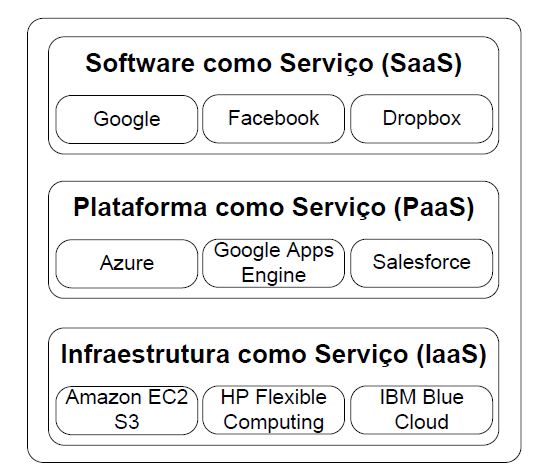
\includegraphics[scale=0.65]{images/modelosdenegocioCN.PNG}
    \caption{Serviços oferecidos em CN
    \cite{batista2016modelos}}
    \label{figuramodelosdenegocio}
\end{figure}

\begin{itemize} 

\item \textbf{\emph{Software as a Service (Saas)}}

Modelo em que o \emph{software} é oferecido por um provedor de serviços, disponível sob demanda, geralmente por meio de um navegador \emph{Web}.

\item \textbf{\emph{Platform as a Service (PaaS)}}

Modelo intermediário em que o software é normalmente desenvolvido através de API's fazendo com que o foco se concentre somente no desenvolvimento do software, salvo algumas configurações necessárias no ambiente.

\item \textbf{\emph{Infrastructure as a Service (IaaS)}}

Modelo em que o hardware é abstraído do usuário através de MVs, fazendo com que o usuário não precise se preocupar com aspectos relacionados a parte física, como servidores e redes.

\end{itemize}
\section{Desafios}\label{subsec:desafios}
%Apesar da CN estar amplamente presente na industria ainda há diversos problemas sendo encontrados constantemente e soluções propostas, nesta seção são apresentados desafios citados em \cite{zhang2010cloud}.
Apesar da CN estar amplamente presente na industria e no desenvolvimento tecnológico, diversas propostas de pesquisa vem sendo consideradas. Nesta seção são apresentados principais desafios da área abordados na literatura~\cite{zhang2010cloud}.

\subsection{Provisionamento automatizado de serviços}
Consiste em alocar e realocar MV de acordo com a necessidade do cliente. As realocações devem ser feitas respeitando os \emph{SLO (Service Level Objetive)} do ambiente e buscando minimizar o custo operacional. Contudo, não é fácil determinar como mapear SLOs para cumprir requisitos de QoS, como por exemplo, definir a utilização da CPU e memória, pois essas oscilam a cada segundo. Justifica-se a necessidade de constantes atualizações e otimizações no sistema \emph{online} para lidar com esses provisionamentos.

\subsection{Migração de Máquina Virtual}

A virtualização trouxe diversas vantagens para a CN, como a possibilidade da criação de MVs com o intuito de balancear a carga por todo o \textit{data center}, e ainda, possibilitando robustez e rápida resposta de provisionamento em \textit{data centers}.

Os principais benefícios da migração de MVs são otimizar uso dos recursos, no entanto, isso não é uma tarefa simples. Atualmente, a detecção de picos de carga de trabalho e o início de uma migração não têm a agilidade necessária para responder às mudanças súbitas e dinâmicas de carga de trabalho.

\subsection{Consolidação de servidores}

A consolidação de servidores é uma maneira eficaz de maximizar a utilização de recursos enquanto minimizamos o consumo energético do ambiente de CN. A técnica de migrar MV em tempo real é constantemente utilizada para consolidar MVs que estão alocadas em múltiplos servidores, frequentemente sub-utilizados. A migração para um único servidor, viabiliza que os outros servidores possam ser desligados. Contudo, o problema de consolidação de servidores em um data center é constantemente avaliado como uma variante do problema do empacotamento (\emph{bin-packing}), apresentado com um problema computacional NP-Difícil~\cite{ferdaus2014virtual} e amplamente conhecido.

\subsection{Gerenciamento de Energia}

Melhorar a eficiência energética é outra questão importante na CN. E empresas de TI estão sobre constante pressão, visando novas tecnologias que permitem diminuir o consumo energético, não só pela questão financeira mas sobretudo para cumprir as regulamentações governamentais e os padrões ambientais.

\section{Simuladores}

Uma das desvantagens da CN está na sua modelagem de ambientes de testes. O usuário final , que espera uma experiência satisfatória do serviço, e no outro lado, as empresas, que não desejam ter gastos desnecessários em energia ou compra demasiada de equipamentos.

Com o intuito de solucionar esse problema foram desenvolvidos simuladores para auxiliar na implementação de ambientes de CN controlados. Há muitos benefícios em utilizarmos simuladores como bem descrito em \cite{ahmed2014cloud}, com destaque nos apresentados na sequência:

\begin{itemize}
    \item[(i)] Custo Mínimo: considere o desenvolvimento via software, gerando muito menor custo quando comparando com hardware.
    \item[(ii)] Repetível e controlável: podemos testar diversificando os testes por várias vezes até obtermos a saída desejável.
    \item[(iii)] Ambientes heterogêneos: fornece avaliação para cenário diversificados sob diferentes cargas de trabalho e medição de custos.
\end{itemize}

%Uma idéia:
Dentre os simuladores citados em \cite{ahmed2014cloud}, nossas escolhas foram motivadas pelo seguintes aspectos: (i) ter amplo emprego científico, (ii) disponibilizar referencial teórico, e principalmente abranger o ponto principal, (iii) apresentar um modelo energético consolidado. 
Os três simuladores e suas principais características são ressaltadas a baixo:

\begin{itemize}
    \item GreenCloud, Proposto em \cite{greencloud} e apresentando um simulador projetado para calculo do consumo de energia em qualquer componente específico do \textit{data center} como \emph{link, switch, gateway}, etc. Porém, requerendo muita memória e  tempo de simulação sendo, então recomendado somente para pequenos \textit{data centers};
    
    \item CloudAnalyst, Proposto em \cite{cloudanalyst} e apresentado um simulador projetado para avaliar a performance e o custo de grandes ambientes de CN distribuídos em diferentes locais e manipulando enorme carga de trabalho do usuário, tem uma interface gráfica que facilita a visualização dos dados através de gráficos
    
    \item CloudSim, Proposto em \cite{calheiros2011cloudsim} e apresentado como simulador com a maior popularidade no contexto de uma comunidade ativa, possibilitando a modelagem e criação de grandes \textit{data centers}, número ilimitado de MVs e suportando o importante recurso do modelo, referido como \emph{pay-as-you-go} da CN.
\end{itemize}

Com o estudo dos simuladores atuais, em especial os três citados acima o simulador escolhido para implementação foi o CloudSim \cite{calheiros2011cloudsim} devido ao seu suporte a simulação energética, baixa utilização de memória possibilitando a simulação de grandes \textit{data centers} e por já conter nativamente diversas políticas de alocação e escalonamento de MVs.


\subsection{CloudSim}
A Figura \ref{fig:cloudsimarchitecture} mostra o projeto de várias camadas da estrutura do software CloudSim e seus componentes de arquitetura. O CloudSim suporta várias funcionalidades, como enfileiramento e processamento de eventos, criação de entidades do sistema da Nuvem, como ,serviços, host, \textit{data center}, \textit{broker}, MVs, incluindo ainda comunicação entre componentes e gerenciamento do relógio de simulação.

\begin{figure}[!htb]
   \centering
    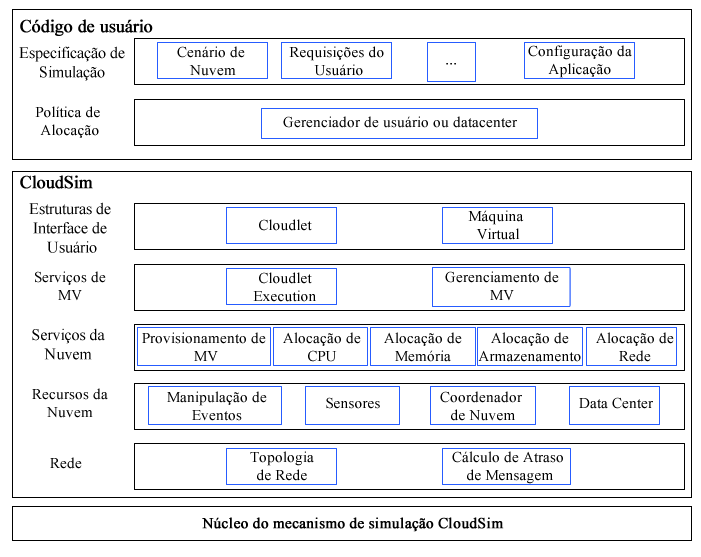
\includegraphics[scale = 0.9]{images/arquiteturaCloudSimPtBr.png}
    \caption{Arquitetura de Camadas do CloudSim. Adaptado de  \cite{calheiros2011cloudsim}}
    \label{fig:cloudsimarchitecture}
\end{figure}

A camada de simulação do CloudSim fornece suporte para modelagem e simulação de ambientes de \textit{data center} virtualizados baseados em nuvem, incluindo interfaces de gerenciamento dedicadas para MVs, memória, armazenamento e largura de banda. Os problemas fundamentais, como provisionamento de hosts para MVs, gerenciamento de execução de aplicativos e monitoramento do estado dinâmico do sistema, também são tratados por essa camada.

Além destes recursos, esta camada também expõe as funcionalidades para o desenvolvimento de aplicativos, executando perfis de carga de trabalho complexos e estudos de desempenho de aplicativos. A camada mais superior na pilha do CloudSim é o Código de usuário, disponibilizando entidades básicas para hosts como (número de máquinas, suas especificações e outras), suporte a aplicativos (número de tarefas e seus requisitos), MVs, número de usuários e seus tipos de aplicativo e políticas de escalonamento.

%A configuração do ambiente de testes e a avaliação do módulo fuzzy para detecção do nível de carga dos hosts na cloud empregou o CloudSim~\cite {calheiros2011cloudsim}, um kit de ferramentas para modelagem e simulação de infraestruturas e serviços de computação em nuvem.

%Neste trabalho o enfoque está na camada de código do usuário (topo), sua função é expor as configurações básicas do ambiente, sendo essas: \textit{hosts} (número de máquinas e suas especificações), aplicações (número de tarefas e suas necessidades), MVs, números de usuários e seus tipos de aplicações, e ainda as políticas de balanceamento.
\begin{comment}
Devido a modelagem energética e ampla comunidade ativa o simulador optou-se em utilizar o CloudSim~\cite {calheiros2011cloudsim}. A Figura~\ref{fig:cloudsimarchitecture} mostra o design multi-camadas da estrutura do software CloudSim e seus componentes arquitetônicos. A camada de código do usuário (topo) tem como função expor as configurações básicas do ambiente, sendo essas: \textit{hosts} (número de máquinas e suas especificações), aplicações (número de tarefas e suas necessidades), MVs, números de usuários e seus tipos de aplicações, e ainda as políticas de balanceamento que serão utilizadas na simulação. Já a camada do CloudSim (inferior) é o mais baixo nível que é possível atingir no CloudSim, caso deseja-se estudar a eficiência de políticas diferentes na alocação de suas MVs (provisionamento de MV), precisaria implementar suas estratégias nessa camada. Essa implementação pode ser feita estendendo-se a principal classe de provisionamento de MV. Essa camada também expõe as funcionalidades que um desenvolvedor de aplicativos em nuvem pode estender em relação a criação de perfil de carga de trabalho complexa de alto desempenho e o estudo de desempenho de aplicativos.
\end{comment}

%Devido a modelagem energética e ampla comunidade ativa optou-se em utilizar o CloudSim~\cite {calheiros2011cloudsim}. A Figura~\ref{fig:cloudsimarchitecture} mostra o design multi-camadas da estrutura do software CloudSim e seus componentes arquitetônicos.

O CloudSim foi escolhido para emprego neste trabalho considerando sua ampla aceitação e uso pela comunidade cientifica. Além disto, fornece em sua estrutura as funcionalidades para o emprego na avaliação energética, da mesma forma proporciona facilidade no controle do ambiente simulado.

%Como foi ressaltado na Seção~\ref{subsec:desafios}, a CN tem diversos desafios a serem tratados, dentre eles está o gerenciamento de recursos visando melhorar a eficiência energética. Na Figura~\ref{fig:taxonomiaenergetica} é apresentado a taxonomia das técnicas que visam uma melhor eficiência energética, nela há duas técnicas principais, uma que trata o ambiente a nível de hardware e outra que por meio da virtualização, cria mais um nível de abstração do ambiente trazendo dois novos ramos, que tratam o gerenciamento a nível de SO ou a nível de Sistema. 
%Em \cite{beloglazov2013energy}, o autor descreve técnicas para gerenciamento

%Na Figura~\ref{fig:taxonomiaenergetica}, é apresentada a taxonomia das técnicas que gerenciam o ambiente de CN baseadas no consumo energético, sendo elas divididas em duas principais, as que tratam de modo estático e dinâmico. As técnicas estáticas contêm todas aquelas otimizações que são implementadas a nível de hardware, sendo elas desenvolvidas no projeto dos circuitos, da parte lógica, arquitetônica ou sistêmica. Otimizações a nível de circuito tem como objetivo a redução da alteração do estado (ligado/desligado) de transistores e portas lógicas, essas otimizações são obtidas através do desenvolvimento de projetos complexos de desenho de portas e redimensionamento dos transistores. Otimizações a nível lógico tem como objetivo diminuir a redução da alteração do estado (ligado/desligado) dos circuitos sequenciais. Otimizações a nível arquitetônico incluem análise do desenho do sistema para posterior aplicação de técnicas de otimização energética. Porém, para essas otimizações a nível de hardware surtirem efeito é essencial considerar a implementação de programas específicos para serem executados, pois mesmo com otimizações a nível de hardware um programa que não satisfaz as propriedades desse hardware pode trazer péssimo desempenho e grande perda energética. 


%%%% Até aqui já foi corrigido pela Renata %%%%


%\subsection{Técnicas para Gerenciamento de Recursos para Eficiência Energética}
\section{Classificação do Gerenciamento de Recursos para Eficiência Energética}

Em \cite{beloglazov2013energy}, define-se uma taxonomia das técnicas para gerenciamento de ambiente de CN que busca a eficiência energética. Essa taxonomia é reapresentada na Figura~\ref{fig:taxonomiaenergetica}. A taxonomia está dividida em duas principais classes  na qual fazem o tratamento do consumo energético de duas formas distintas. (i) modo estático, e (ii) dinâmico. 

\begin{figure}[!htb]
   \centering
    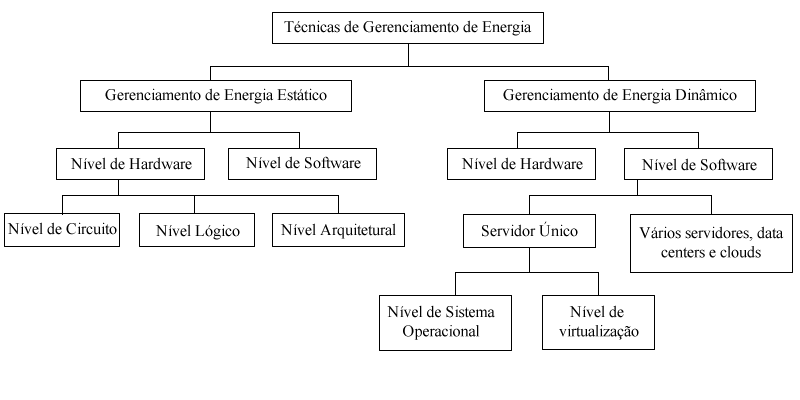
\includegraphics[scale = 0.78]{images/taxonomia/taxonomiaEnergetica.png}
    \caption{Taxonomia do gerenciamento de recursos. Adaptado de  \cite{beloglazov2013energy}}
    \label{fig:taxonomiaenergetica}
\end{figure}

As técnicas estáticas contêm todas aquelas otimizações que são implementadas a nível de hardware, sendo estas desenvolvidas no projeto dos circuitos, da parte lógica, arquitetônica ou sistêmica. 

Aprimoramentos a nível de circuito tem como objetivo a redução da alteração do estado (ligado/desligado) de transistores e portas lógicas, essas otimizações são obtidas através do desenvolvimento de projetos complexos de desenho de portas, e incluindo o redimensionamento dos transistores. 

Otimizações a nível lógico tem como objetivo diminuir a redução da alteração do estado (ligado/desligado) dos circuitos sequenciais. Otimizações a nível arquitetônico incluem análise do desenho do sistema para posterior aplicação de técnicas de otimização energética. Porém, para essas otimizações a nível de hardware surtirem efeito é essencial considerar a implementação de programas específicos para serem executados, pois mesmo com otimizações a nível de hardware, um programa que não satisfaz as propriedades desse hardware pode trazer degradação de desempenho, e redução da eficiência energética.
 
%Como apresentado na Seção~\ref{sec:caracteristicas}, a CN tem como objetivo abstrair a manipulação física dos servidores aos usuários e dar liberdade sobre como utilizarão o ambiente, criando heterogeneidade do ambiente, tanto nas cargas de trabalho, quanto no tipo de operação (CPU, RAM, I/O). Para obter  eficiência energética, é necessário o desenvolvimento de técnicas que se adaptam as necessidades e aos comportamentos diferentes do ambiente, para isso, são desenvolvidas técnicas que tratam o ambiente de modo dinâmico, adaptando-se de acordo com o comportamento do ambiente, e ainda, dividir essas técnicas dinâmicas em nível de hardware, e software. 
Como apresentado na Seção~\ref{sec:caracteristicas}, a CN tem como objetivo abstrair a manipulação física dos servidores aos usuários e dar liberdade sobre como utilizarão o ambiente, criando heterogeneidade do ambiente, tanto nas cargas de trabalho, quanto no tipo de operação (CPU, RAM, I/O). 

Para obter eficiência energética, é necessário o desenvolvimento de técnicas que se adaptam às necessidades e aos comportamentos diferentes do ambiente, são desenvolvidas técnicas que tratam o ambiente de modo dinâmico, adaptando-se de acordo com o comportamento do ambiente, estas técnicas, são ainda divididas nas seguintes sub-categorias: (i) dinâmicas em nível de hardware, e (ii) software. 

Técnicas dinâmicas a nível de hardware normalmente podem ser classificadas em técnicas de escalonamento dinâmico de desempenho, variação de tensão e escala de frequência, ou ainda, desligamento parcial ou completo de componentes em determinados períodos. Já técnicas a nível de software possibilitam ao administrador do ambiente optar por diferentes políticas de acordo com a necessidade. 

A camada de software é dividida em outras duas, que são as camada de Sistema Operacional (SO) e Virtualização. Técnicas dinâmicas que operam no nível de Sistema Operacional tem como intuito fazer com que a camada de software auxilie na obtenção de determinados objetivos, podendo eles serem: (i) adaptar a aplicação ao ambiente, (ii) otimizar a utilização dos recursos do sistema, (iii) aplicar técnicas de economia de energia, e (iv) manipular as cargas de trabalho. 

A outra camada é a de virtualização, que acrescenta uma camada de abstração entre o sistema operacional e o hardware, possibilitando a criação de MVs com o intuito de otimizar a utilização dos recursos.

Finalmente, tem-se a camada de múltiplos servidores e \textit{data centers} foco da pesquisa neste trabalho. Técnicas nesse nível tem por objetivo usufruir da heterogeneidade presente nesses ambientes, estendendo as práticas de um único servidor para diversos servidores. Normalmente, tem-se um gerenciador global e algumas operações sendo realizadas internamente nas máquinas para evitar sobrecarga do gerenciador global.


\chapter{Lógica Fuzzy} \label{sec:fuzzy}

A LF está fundamentada na Teoria dos Conjuntos Fuzzy (TCF) introduzida por Zadeh~\cite{zadeh1965, zadeh2008there}, estendendo os conceitos da Lógica Clássica. Diferentemente da rigidez Booleana na avaliação de argumentos, a LF promove a flexibilidade da relação de pertinência, ao considerar graus intermediários de pertinência no intervalo unitário [0,1], fornecendo técnicas poderosas de modelagem para o tratamento de informações vagas ou imprecisas. 

Esta seção apresenta a fundamentação teórica a partir de conceitos da LF, fazendo correlação entre LF e lógica clássica. Reporta-se também uma extensão dos conjuntos fuzzy, os conjuntos fuzzy valorados intervalarmente.

\section{Lógica Clássica x Lógica Fuzzy}

Na Lógica Clássica só é possível assumir dois valores para a pertinência de um elemento a um conjunto: verdadeiro (1) e falso (0). Entretanto, na abordagem fuzzy pode-se assumir valores num intervalo de 0 a 1,  flexibilizando a modelagem e, também, a aplicação dos valores podem ser expressos em termos linguísticos, aproximando-os da linguagem natural. Alguns exemplos são as expressões: alto, baixo, médio, muito alto, muito baixo, pouco alto, pouco baixo, etc. Esse tipo de modelagem, em processos mais complexos, permite resultados mais acurados, melhorando o desempenho quando da tomada de decisão (\emph{Multiple criteria decision making} - MCDM). 

Na TCF, todo conjunto está identificado por sua função de pertinência. Assim cada elemento $x$ de um conjunto universo $\chi\neq\varnothing$ está associado a um conjunto fuzzy $A$  definido pela função de pertinência $\mu_A:\chi \rightarrow [0,1]$. Neste contexto, um conjunto fuzzy tipo-1 (T1FS) A é dado pela expressão
\begin{equation}
A= \{(x, \mu_A(x)) \colon  x \in \chi\}.
\end{equation}

Em outras palavras, um conjunto universo que representa todos os alunos de uma sala, e um subconjunto desse universo, que seria os que são bons em matemática.

Todos os elementos do conjunto universo teriam um grau de pertinência, referente a esse subconjunto, que significaria o quanto cada elemento é bom em matemática, em sendo então valorado no um intervalo de 0 a 1. Por exemplo, se um elemento tivesse um grau de pertinência 0, ele não seria bom em matématica e se tivesse 1 ele seria muito bom em matématica, e se tivesse um 0,8 ele seria somente bom em matématica. Essa forma de modelar é diferente do modelo clássico, onde só poderia ser classificados em bons em matemática (1) e ruins em matemática(0).

\section{Fundamentos da Lógica Fuzzy}

A Lógica Fuzzy está baseada na Teoria dos Conjuntos Fuzzy, incorporando o conceito de pertinência, onde os elementos tem um grau de pertinência a um conjunto fuzzy.

Formalmente um conjunto fuzzy A é caracterizado por uma função de pertinência $\mu_A : \chi \rightarrow [0,1]$, a qual associa a cada elemento de um universo $\chi \neg \emptyset$, um número real no intervalo unitário$[0,1]$:
\begin{equation}
    A = \{ (x,\mu_{A}(x))  ~|~  ~x\in \chi \mbox{   e   } \mu_{A}(x) \in [0,1] \}, 
\end{equation}
e, para $x\in \mathbf{U}, ~\mu_A(x)$ representa o grau de pertinência de $x$ em $A$. 
  
\subsection{Conectivos da Lógica Fuzzy}

\begin{Def}
A função $N:[0,1] \rightarrow [0,1]$ é uma \emph{negação fuzzy} se verifica as seguintes propriedades:
\begin{description}
\item [$N_1$]: $N(0) = 1$ e  $N(1) = 0$;

\item [$N_2$]: Se $x \geq y$ então $N(x)\leq N(y)$, $\forall x,y \in [0,1]$.
\end{description} 
\end{Def}
Uma negação fuzzy que também satisfaz a propriedade involutiva 
\begin{description}
\item [$N_3$]: $N(N(x))=x$, $\forall x \in \mathbf{U}$.
\end{description}
é chamada de negação fuzzy forte.
 
\newpage

Apresentam-se a seguir as principais definições de negações fuzzy:
\begin{enumerate}
\item \textbf{Negação Complementar ou Negação Padrão}, negação forte dada por~~
\begin{equation}\label{ex-st-neg}N_C(x)=1-x.\end{equation}


\item \textbf{Negações de Gödel}, as quais são negações fuzzy, mas não são fortes:
\begin{equation}
N_{D1}(x)=
\left \{
\begin{array}{ll}
0,            & \mbox{ se $x > 0$} \\
1 , & \mbox{ se x = 0;}
\end{array}
\right. \,\, 
N_{D2}(x)=
\left \{
\begin{array}{ll}
1,            & \mbox{ se $x < 1$} \\
0 , & \mbox{ se x = 1;}
\end{array}
\right.
\end{equation}
\end{enumerate}

Uma negação fuzzy é utilizada geralmente para representar o operador decomplemento entre conjuntos fuzzy:
\begin{equation}
A_C  = \{ ( x,\mu_{A_C} ) : x \in \mathbf{U} \mbox{  e } \mu_{A_C}(x)=N(\mu_{A}(x)) \}.
\end{equation}
 
\begin{Def}\label{defnorma}  Uma norma triangular, conhecida como t-norma, é uma operação binária $T:[0,1]^2~\rightarrow~[0,1]$ tal que, $ \forall x,y, z\in [0,1]$,  as seguintes propriedades são verificadas:
\begin{description}
  \item [$T_1$] Comutatividade:~~~~~$T(x,y) = T(x,y)$;
  \item [$T_2$] Associatividade:~~~~~$T(x(T(y,z))=T(T(x,y),z)$;
  \item [$T_3$] Elemento Neutro:~~~~$T(x,1)=x$;
  \item [$T_4$] Monotonicidade:~~~~~$T(x,y)\leq T(x,z)$~~~se~~$y\leq z$.
\end{description}
\end{Def}

Uma t-norma é utilizada geralmente para representar o operador de conjunção (e) ou a intersecção entre conjuntos fuzzy:
\begin{equation}
A \cap B = \{ ( x,\mu_{A \cap B} ) : x \in \mathbf{U} \mbox{  e } \mu_{A \cap B}(x)=T(\mu_{A}(x),\mu_{B}(x)) \}.
\end{equation}

\newpage

A Tabela~\ref{tabexpnormas} apresenta exemplos de t-normas.


\begin{center}
\begin{table}
\caption{{\small Exemplos básicos de  t-normas}}
\label{tabexpnormas}
\centering
\begin{tabular}{ll}
\hline
Designação & Representação \\
\hline
$T_{M}$: Mínimo&  $T_{M}=min(x,y)$   \\
$T_{P}$: Produto&  $T_{P}=xy$   \\
$T_{L}$: Lukasiewicz&  $T_{L}=max(x+y-1,0)$  \\
$T_{D}$: Drástica do produto &
{\small $ T_{D} =(x,y)=
\left \{
\begin{array}{ll}
0,            & \mbox{ se $x,y \in [o,1[$;} \\
\min (x,y),   & \mbox{ c.c.}
\end{array}
\right.$}  \\
$T_{nM}$: Nilpotente mínimo & {\small $T_{nM}(x,y)=
\left \{
\begin{array}{ll}
0,            & \mbox{ se $x +y \leq 1$;} \\
\min (x,y), & \mbox{ c.c.}
\end{array}
\right.$} \\
\hline
\end{tabular}
\end{table}
\end{center}

\begin{Def} Seja o intervalo unitário real $[0,1]\subseteq \mathbf{R}$. Uma conorma triangular, indicada por t-conorma, é uma operação binária $S:[0,1]^2~\rightarrow~[0,1]$ que satisfaz as seguintes propriedades:
\begin{description}
  \item [$S_1$] Comutatividade:~~~~~$S(x,y) = S(x,y)$;
  \item [$S_2$] Associatividade:~~~~~$S(x(S(y,z))=S(S(x,y),z)$;
  \item [$S_3$] Elemento Neutro:~~~~$S(x,0)=x$;
  \item [$S_4$] Monotonicidade:~~~~~$S(x,y)\leq S(x,z)$ se $y\leq z$.
\end{description}
\end{Def}
Uma t-conorma é utilizada geralmente para representar o operador de disjunção (ou) ou a união entre conjuntos fuzzy:
\begin{equation}
A \cup B = \{ ( x,\mu_{A \cup B} ) : x \in \mathbf{U} \mbox{  e } \mu_{A \cup B}(x)=S(\mu_{A}(x),\mu_{B}(x)) \}.
\end{equation}

Este trabalho também considera o estudo do operador OWA~\cite{yager2004generalized}, provendo um meio de agregar valores associados à satisfação de múltiplos critérios, e, ainda, unificando ambos os comportamentos de elementos em conjunto fuzzy, o conjuntivo e o disjuntivo. Operadores OWA são funções de agregação comutativos, idempontentes e apresentam um comportamento compensatório. \cite{yager2004owa}

A agregação obtida pela aplicação de um operador OWA está entre os valores máximo e mínimo. Esse operador generaliza o mínimo e o máximo, podendo ser visto como uma função parametrizada variando no intervalo unitário [0,1].

\begin{Def}
Seja $\sigma \colon N_n \rightarrow N_n$ uma permutação consistindo na ordenação não decrescente, ou seja, 
$0\leq x_{\sigma(1)} \leq x_{\sigma(2)} \leq \ldots \leq x_{\sigma(n)} \leq 1$,  $0 \leq w_{i} \leq 1$ e $\sum_{i=1}^{n} w_{i}=1$. Um operador \mbox{$OWA \colon [0,1]^n \rightarrow [0,1]$} é definido pela expressão:\vspace{-0.2cm}
\begin{eqnarray}\label{eq-OWA}
 OWA(x_{1},x_{2},...,x_{n}) &=& \sum_{j=1}^{n} w_{j} x_{\sigma(j)}
\end{eqnarray}
\end{Def}

A partir de um operador OWA, tem-se uma família parametrizada de operadores de agregação incluindo o máximo, o mínimo, a mediana e a média aritmética, os quais são gerados por escolhas de parâmetros.

\subsection{Números Fuzzy}
Assim como no caso clássico, também temos o objetivo de fazer algebras a partir da estrutura lógica das T2FS. A diferença é que se pretende calcular quantidades imprecisas. Por exemplo, é opinião unânime dizer que o dobro de uma quantidade `em torno de 15' resulta em outra `em torno de 30'. Para isto, construíram-se objetos matemáticos que generalizam os números reais. Tais objetos serão chamados de números fuzzy \cite{george2008fuzzy}.

As principais definições e propriedades de números são apresentadas logo a seguir.

\begin{Def}
Um conjunto fuzzy F é chamado número fuzzy quando o conjunto universo, onde F está definido, é o conjunto dos números reais $\mathbb{R}$ e a função de pertinência $\mu_{F} : \mathbb{R} \longrightarrow [0,1]$, é tal que: \\

\textbf{1.} $\mu_{F}(x) \mbox{ atinge o 1, isto é, } \sup\limits_{x\in\mathbb{R}} \mu_{F}(x)=1.$ \\


\textbf{2.} $[F]^{\alpha}$ é um intervalo fechado, $\forall \alpha \in (0,1].$ \\

\textbf{3.} $\mbox{O suporte de F é limitado.}$ \\

Os números fuzzy mais comuns são triangulares, trapezoidais e senoidais.

\end{Def}


\begin{Def}
Um número fuzzy F é dito triangular se sua função de pertinência é da forma aprsentada na Eq. \ref{eq:numerofuzzy}.

\begin{equation} \label{eq:numerofuzzy}
 \mu_{F}(x)=
  \left \{
   \begin{array}{ll}
  0,  & \mbox{ se $x \leq a,$} \\
  \frac{x-a}{m-a}, & \mbox{ se $a < x \leq m,$} \\
  \frac{x-b}{m-b}, & \mbox{ se $m < x \leq b,$} \\
  0, & \mbox{ caso contrário.}
   \end{array}
  \right.
\end{equation} 
O gráfico da função de pertinência de um número fuzzy triangular tem a forma de um triângulo, tendo como base o intervalo $[a,b]$ e, como único vértice fora desta base, o ponto $(m,1)$. Deste modo, os números reais $a,~m ~e~ b$ definem o número fuzzy triangular F, graficamente representado na Figura~\ref{fig:NFuzzyTriangular}.
\begin{figure}[ht]
\centering
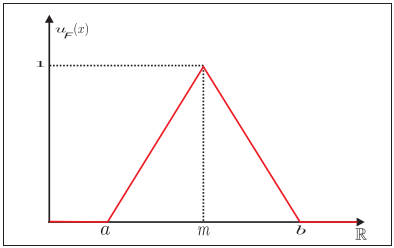
\includegraphics[scale=0.5]{images/numero_fuzzy_triangular.png}
 \captionof{figure}{Número fuzzy triangular}
\label{fig:NFuzzyTriangular}
\end{figure}

\end{Def}

\newpage

\begin{Def}
Um número fuzzy F é dito trapezoidal se sua função de pertinência tem a forma de um trapézio, com expressão algébrica dada na Eq.\ref{eq:numerofuzzy2} e graficamente apresentada na Figura \ref{fig:NFuzzyTrapeziodal}.
\begin{equation}\label{eq:numerofuzzy2}
 \mu_{F}(x)=
  \left \{
   \begin{array}{ll}
  \frac{x-a}{b-a},  & \mbox{ se $a \leq x < b,$} \\
  1, & \mbox{ se $b \leq x \leq c,$} \\
  \frac{d-x}{d-c}, & \mbox{ se $c < x \leq d,$} \\
  0, & \mbox{ caso contrário.}
   \end{array}
  \right.
\end{equation}
\begin{figure}[ht]
\centering
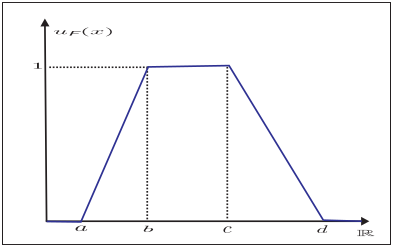
\includegraphics[scale=0.5]{images/numero_fuzzy_trapezoidal.png}
 \captionof{figure}{Número fuzzy trapezoidal}
\label{fig:NFuzzyTrapeziodal}
\end{figure}
\end{Def}



\begin{Def} \label{def:senoildal}
Um número fuzzy tem forma senoidal se a função de pertinência for suave e simétrica em relação ao número real. 
A seguinte expressão analítica da função de pertinência da Eq.11 verifica as propriedades da Definição \ref{def:senoildal} para $n, ~a~$ e $\delta \in \mathbb{R}$ dados. Veja a correspondente representação gráfica na Figura \ref{fig:NFuzzySino}.
\begin{equation} \label{eq:numerofuzzysenoidal}
 \mu_{F}(x)=
  \left \{
   \begin{array}{ll}
  \exp(-(\frac{x-n}{a})^{2}),  & \mbox{ se $n - \delta \leq x < n + \delta,$} \\
  0, & \mbox{ caso contrário.}
   \end{array}
  \right.
\end{equation}
\begin{figure}[ht]
\centering
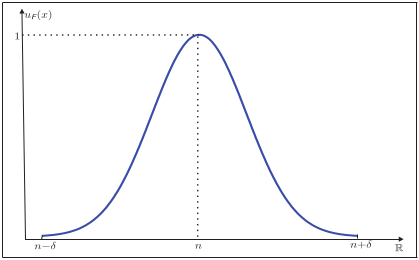
\includegraphics[scale=0.485]{images/numero_fuzzy_sino.png}
 \captionof{figure}{Número fuzzy senoidal}
\label{fig:NFuzzySino}
\end{figure}

\end{Def}


\begin{Def}
Seja F um conjunto fuzzy. O Kernel de F é o conjunto de todos os elementos $x \in U$ cujo grau de pertinência é 1, isto é, $Ker(F)= \{x \in U: \mu_{F}(x)=1\}.$
\end{Def}

\begin{Def}
Um elemento $x \in U$, no qual $\mu_{F}(x)=0.5$ é denominado, ponto crossover.
\end{Def}

\begin{Def}
Um conjunto F cujo suporte é um único ponto em $U$, com $\mu_{F}(x)=1,$ é denominado, singleton fuzzy.
\end{Def}

\begin{Def}
A altura de um conjunto fuzzy F é o valor máximo da pertinência de $x$ em $U$, isto é, $hgt(F) = \sup\limits_{x \in U} \mu_{F}(x)$.

A Figura \ref{fig:AltKerSupCF} apresenta a identificação da altura, kernel e suporte de um conjunto fuzzy.

\begin{figure}[ht]
\centering
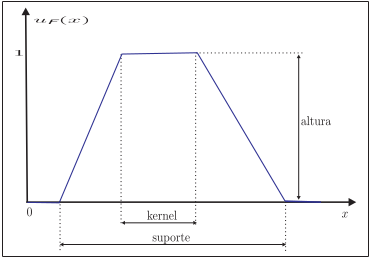
\includegraphics[scale=0.55]{images/altura_kernel_cf.png}
 \captionof{figure}{Altura, Kernel e suporte de um conjunto fuzzy}
 %\\ Fonte: \cite{rizol2011logica}.
\label{fig:AltKerSupCF}
\end{figure}

\end{Def}

\subsection{Implicações Fuzzy}

A literatura apresenta uma diversidade de definições e aplicações no assunto de implicações fuzzy e suas duais \cite{baczynski2004residual, baczynski2008introduction, balasubramaniam2007yager}. Sendo a implicação fuzzy uma generalização da abordagem clássica, o único consenso em suas definições é que a implicação fuzzy deve ter o mesmo comportamento da implicação clássica quando os valores de entrada da implicação forem uma combinação dos extremos do intervalo $[0,1]$. As implicações estão contidas no conjunto das subimplicações fuzzy, as quais são operadores que não verificam totalmente o comportamento da implicação clássica.

Um operador binário $I : U^{2} \rightarrow U$ é uma \textbf{implicação fuzzy} se $I$ satisfaz as condições de contorno, (\textbf{I2} e \textbf{I3}) : \\ \\
\textbf{I0:} $I(1,1)=I(0,1)=I(0,0)=1$. \\
\textbf{I1:} $I(1,0)=0$. \\
\textbf{I2:} Se $x \leq z$ então $I(x,y) \geq I(z,y)$ (antitonicidade no primeiro argumento); \\
\textbf{I3:} Se $y \leq z$ então $I(x,y) \leq I(x,z)$ (isotonicidade no segundo argumento); 


\section{Fundamentos da Lógica Fuzzy Valorada Intervalarmente}

Nesta sessão apresentam-se os conceitos básicos da lógica fuzzy valorada intervalarmente (IVFL), na qual são atribuídos não um número mas um outro conjunto do tipo intervalo como grau de pertinência associado a um elemento do universo.

Um conjunto fuzzy valorado intervalarmente (IVFS) é um caso particular de (T2FS).

\subsection{Conjuntos Fuzzy Tipo 2}

A teoria dos conjuntos fuzzy tipo 2 (T2FS) foi introduzida por \cite{zadeh1975concept} como uma extensão do conjunto fuzzy tradicional. T2FS são conjuntos fuzzy, com grau de pertinência em um T1FS.

A T2FS, modela a incerteza na definição do grau de pertinência. No caso especial dos conjuntos fuzzy da IVFL, a incerteza entre dois valores fuzzy $0.3$ e $0.4$ resulta em atribuir [$0.3,0.4$] como grau de pertinência. As inferências baseadas em T2FL permitem que se aplique o Sistema Baseado em Regras Fuzzy Tipo 2.

Um elemento do tipo T2FS é caracterizado por uma função de pertinência em T2FS, onde seu grau de pertinência passa a ser um conjunto de pares ordenados constituídos por T1FSs.

\begin{Def} \label{defconjtipo2}
Um T2FS $\tilde{A}$, é caracterizado por uma função de pertinência $\mu_{\tilde{A}}(x,u)$, onde $x \in X$ e $u \in J_{x} \subseteq [0,1]$, ou seja:

\begin{equation}
\tilde{A} = \{((x,u), \mu_{\tilde{A}}(x,u)): \forall x \in X, \forall u \in J_{x} \subseteq [0,1] \},
\end{equation}
onde, $0 \leq \mu_{\tilde{A}}(x,u) \leq 1.$
\end{Def}


\begin{Def}
T2FS se reduzem a IVFS quando $\mu_{\tilde{A}}(x,u)=1.$

Um meio de representar T2FS é através da forma geométrica de sua função de pertinência. As Figuras \ref{fig:cf_tipo2_intervalar1}, e \ref{fig:cf_tipo2_intervalar2} mostram IVFS e suas respectivas áreas coloridas em azul correspondem a região denominada {Foot print of Uncertainty}'' (FOU).
\end{Def}


\begin{figure}[h]
\subfigure[\label{fig:cf_tipo2_intervalar1}]{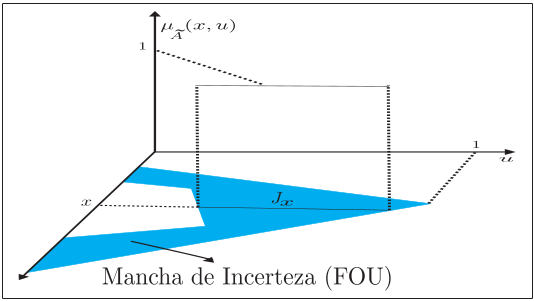
\includegraphics[scale =0.438]{images/cf_tipo2_intervalar.png}}
\subfigure[\label{fig:cf_tipo2_intervalar2}]{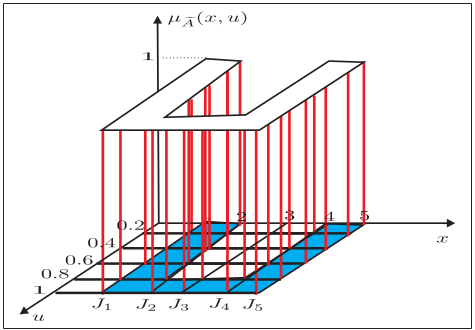
\includegraphics[scale =0.4]{images/cf_tipo_intervalar22.png}}
\caption{Conjuntos Fuzzy Tipo 2 Intervalar.}\label{fig:cf_tipo_intervalar2}
\end{figure}

O grau secundário dos T2FS é sempre igual a 1. Portanto, a terceira dimensão acaba não mostrando nenhuma informação adicional e um T2FS pode sempre ser representado apenas por sua região de FOU. As Figuras \ref{fig:fp_triangular_t2}, \ref{fig:fp_trapezoidal_t2}, \ref{fig:fp_gaussiano_t2} e \ref{fig:fp_singleton_t2}, apresentam várias formas de T2FS: intervalar, triangular, trapezoidal, gaussiano e ``singlenton'', respectivamente. 


\begin{figure}[h]
\subfigure[Triangular\label{fig:fp_triangular_t2}]{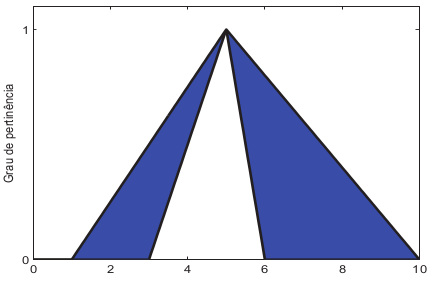
\includegraphics[scale =0.5]{images/fp_triangular_t2.png}}
\subfigure[Trapeziodal\label{fig:fp_trapezoidal_t2}]{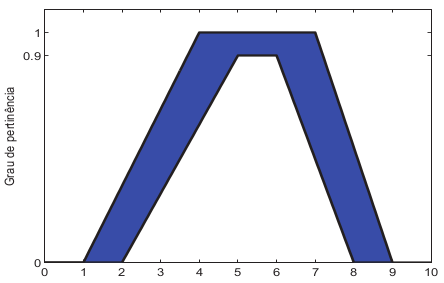
\includegraphics[scale =0.51]{images/fp_trapezoidal_t2.png}}
\subfigure[Gaussiano\label{fig:fp_gaussiano_t2}]{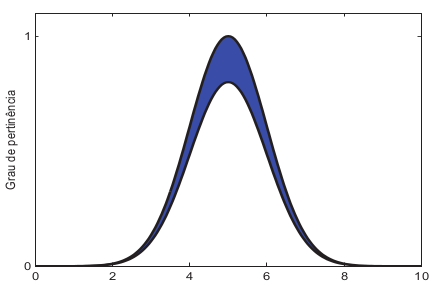
\includegraphics[scale =0.5]{images/fp_gaussiano_t2.png}}
\subfigure[Singleton\label{fig:fp_singleton_t2}]{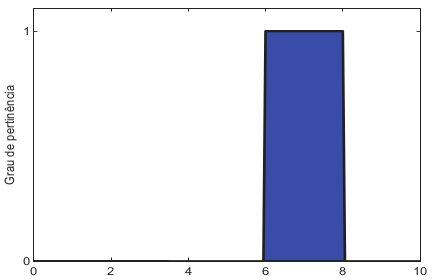
\includegraphics[scale =0.51]{images/fp_singleton_t2.png}}
\caption{Exemplos de conjuntos fuzzy do tipo 2 intervalares.}\label{fig:conj}
\end{figure}

\begin{Def}
O corte vertical de $\mu_{\tilde{A}}(x,u)$ é definido como sendo o plano bidimensional para plano $x = x^{'}$, cujos eixos são $u$ e $\mu_{\tilde{A}}(x^{'},u)$. 
\end{Def}


\begin{Def}
A função de pertinência secundária é o corte vertical de $\mu_{\tilde{A}}(x,u)$ em determinado valor de $x = x^{'}$. Como mostra, a Figura~\ref{fig:fp_secundaria_sf_t2}.

\begin{figure}[!h]
\centering
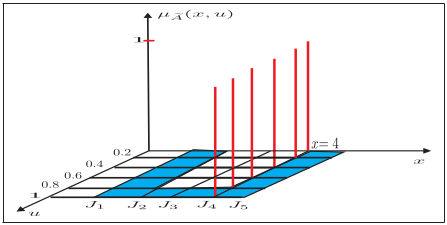
\includegraphics[scale=0.55]{images/fp_secundaria_sf_t2.png}
\caption{Função de pertinência secundária intervalar em x=4.} %\cite{rizol2011logica}
\label{fig:fp_secundaria_sf_t2}
\end{figure} 

\end{Def}

\begin{Def}
A pertinência primária $J_{x}$ de $x$, é definida como o domínio da função de pertinência secundária para o valor de $x$, com $J_{x}=[\underline{J}_{x},\overline{J}_{x}]\subseteq [0,1]$, $\forall x \in  X$.
\end{Def}

\begin{Def}
A ``mancha'' de incerteza (FOU) é definida como a união de todas as pertinências primárias, isto é,
\begin{equation}
FOU(\tilde{A})= \bigcup_{x \in X} (x, j_{x})
\end{equation}
a FOU é um conjunto fuzzy do tipo 2 delimitada por uma função de pertinência do tipo 1 superior e inferior \citep{rizol2011logica}.
\end{Def}

\begin{Def}

A função de pertinência superior é representada na forma $\overline{\mu}_{\tilde{A}}(x), \forall (x) \in X,$ e dada pela expressão abaixo:
\begin{equation}
\overline{\mu}_{\tilde{A}}(x) = \bigcup_{x \in X} (x, \overline{J}_{x}),
\end{equation}logo, a função de pertinência inferior é representada na forma $\underline{\mu}_{\tilde{A}}(x), \forall (x) \in X,$ dados por:
\begin{equation}
\underline{\mu}_{\tilde{A}}(x) = \bigcup_{x \in X} (x, \underline{J}_{x})
\end{equation}onde $\bigcup$ representa o operador de união.
\end{Def}

A Figura \ref{fig:cf_tipo2} exemplifica uma FOU e funções de pertinência superior e inferior.

\begin{figure}[h]
\centering
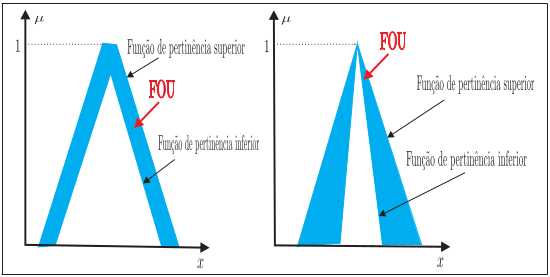
\includegraphics[scale=0.6]{images/cf_tipo2.png}
\caption{Conjunto fuzzy do tipo 2.} % \cite{rizol2011logica}
\label{fig:cf_tipo2}
\end{figure}


\subsection{Conectivos da Lógica Fuzzy Valorada Intervalarmente}

Seja $\mathbb{U}=\{[a,b]~|~0\leq a\leq b\leq 1\}$ o conjunto dos intervalos de reais entre  0 e 1, ou seja, dos valores fuzzy intervalares. Considerando-se que $X \in \mathbb{U}$ então, a partir das funções de projeção, $X=[\underline{X},\overline{X}]$ representa o grau de pertinencia de um elemento num conjunto fuzzy valorado intervalarmente.

\newpage

\begin{Def}\label{theo-neg}
Uma função intervalar $\mathbb{N}:\mathbb{U}\rightarrow
\mathbb{U}$ é uma \textbf{negação fuzzy valorada intervalarmente} se, para todo
$X,Y \in \mathbb{U}$, as seguintes condições são satisfeitas:
\begin{description}
   \item $\mathbb{N}$1: $\mathbb{N}([0,0]) = [1,1]$ e $\mathbb{N}([1,1]) = [0,0]$;
   \item $\mathbb{N}$2a: Se $X \geq Y$ então $\mathbb{N}(X)\leq
   \mathbb{N}(Y)$;
   \item $\mathbb{N}$2b: Se $X\subseteq Y$ então $\mathbb{N}(X)\supseteq \mathbb{N}(Y)$.
\end{description}
Se $\mathbb{N}$ também satisfaz a propriedade involutiva, 
\begin{description}
\item $\mathbb{N}$3: $\mathbb{N}(\mathbb{N}(X)) = X$.
\end{description}
$\mathbb{N}$
é uma \textbf{negação fuzzy valorada intervalarmente forte}.
\end{Def}

Seja $N: U \rightarrow U$ uma negação fuzzy. Então $\mathbb{N}$
é negação fuzzy intervalar representável se $\mathbb{N}$ é dada pela expressão:
\begin{equation}\label{eq-int-n}
\mathbb{N}(X)=[N(\overline{X}),N(\underline{X})].
\end{equation}

Pela Eq.(\ref{eq-int-n}), a extensão intervalar da negação padrão é dada por:
\begin{equation}\label{eq-int-n}
\mathbb{N}_S(X)=[1-\overline{X},1-\underline{X}].
\end{equation}

\begin{Def} Uma norma triangular valorada intervalarmente, conhecida como t-norma intervalar, é uma operação binária $\mathbb{T}:[0,1]^2~\rightarrow~[0,1]$, que satisfaz as seguintes propriedades:
\begin{description}
  \item [$\mathbb{T}_1$] Comutatividade:~~~~~$\mathbb{T}(X,Y) = \mathbb{T}(Y,X)$
  \item [$\mathbb{T}_2$] Associatividade:~~~~~$\mathbb{T}(X(\mathbb{T}(Y,Z))=\mathbb{T}(\mathbb{T}(X,Y),Z)$
  \item [$\mathbb{T}_3$] Elemento Neutro:~~~~$\mathbb{T}(X,[1,1])=X$
  \item [$\mathbb{T}_4$] Monotonicidade em relação às ordens:\\
  A) Produto: $\mathbb{T}(X,Y)\leq \mathbb{T}(Z,W)$~~~se~~$X\leq Z$~~e~~ $Y\leq W$\\
  B) Inclusão: $\mathbb{T}(X,Y)\subseteq \mathbb{T}(Z,W)$~~~se~~$X\subseteq Z$~~e~~$Y\subseteq W$
\end{description}
\end{Def}

Se $T:[0,1]^2\rightarrow [0,1]$ é uma t-norma, então $\mathbb{T}:[0,1]^2\rightarrow [0,1]$ definida por
\begin{eqnarray}\label{eqTI}
\mathbb{T}(X,Y)=[T(\underline{X},\underline{Y}),T(\overline{X},\overline{Y})]
\end{eqnarray}
é uma t-norma intervalar, denominada de t-norma intervalar representável por $T$.




\begin{Def}  Uma conorma triangular intervalar, conhecida como t-conorma intervalar, é uma operação binária $\mathbb{S}:[0,1]^2~\rightarrow~[0,1]$,que satisfaz as seguintes propriedades:
\begin{description}
  \item [$\mathbb{S}_1$] Comutatividade:~~~~~$\mathbb{S}(X,Y) = \mathbb{S}(Y,X)$
  \item [$\mathbb{S}_2$] Associatividade:~~~~~$\mathbb{S}(X((Y,Z))= \mathbb{S}(X,Y),Z)$
  \item [$\mathbb{S}_3$] Elemento Neutro:~~~~$\mathbb{S}(X,[0,0])=X$
  \item [$\mathbb{S}_4$] Monotonicidade  em relação à ordem:\\
  A)Produto: $\mathbb{S}(X,Y)\leq \mathbb{S}(Z,W)$~~~se~~$X\leq Z$~~e~~ $Y\leq W$\\
  B)Inclusão: $\mathbb{S}(X,Y)\subseteq \mathbb{S}(Z,W)$~~~se~~$X\subseteq Z$~~e~~$Y\subseteq W$
\end{description}
\end{Def}

Se $S:[0,1]^2\rightarrow [0,1]$ é uma t-conorma, então $\mathbb{S}:[0,1]^2\rightarrow [0,1]$ definida por
\begin{eqnarray}\label{eqTI}
\mathbb{S}(X,Y)=[S(\underline{X},\underline{Y}),S(\overline{X},\overline{Y})]
\end{eqnarray}
é uma t-conorma intervalar, denominada de t-conorma intervalar representável por $T$.

\begin{center}
\begin{table}[!h]
\caption{{\small Exemplos de t-normas intervalares}}
\centering
\label{tabnormasint}
\begin{tabular}{ll}
\hline
Designação & Representação  \\
\hline
$\mathbb{T}_{M}$:t-norma do Mínimo&  $\mathbb{T}_{M}(X,Y)=min(X,Y)$  \\
$\mathbb{T}_{P}$:t-norma Produto&  $\mathbb{T}_{P}(X,Y)=X\cdot Y$  \\
$\mathbb{T}_{L}$: t-norma de Lukasiewicz&  $\mathbb{T}_{L}(X,Y)=max(X+Y-[1,1],[0,0])$   \\
\hline
\end{tabular}
\end{table}
\end{center}

\begin{center}
\begin{table}[h]
\caption{{\small Exemplos básicos de t-conormas intervalares}}
\centering
\label{tabconormasint}
\begin{tabular}{ll} \hline


Designação & Representação  \\
\hline
$\mathbb{S}_{M}$: t-conorma do Máximo&  $\mathbb{S}_{M}(X,Y)=max(X,Y)$   \\
$\mathbb{S}_{P}$:t-conorma Soma Produto &  $\mathbb{S}_{P}(X,Y)=X+Y-X\cdot Y$   \\
$\mathbb{S}_{L}$:t-conorma de  Lukasiewicz&  $\mathbb{S}_{L}(X,Y)=min(X+Y,[1,1])$  \\
\hline
\end{tabular}
\end{table}
\end{center}

Outros conectivos da Lógica Fuzzy Valorada Intervalarmente podem ser também definidos de forma análoga.

\subsection{Sistema Baseado em Regras Fuzzy Tipo 2}

O Sistema Baseado em Regras Fuzzy Tipo 2 (SBRF2) é utilizado em aplicações onde existe incerteza na determinação exata do grau de pertinência e em aplicações onde não existe alta confiança no modelo \citep{rizol2011logica}.
O diagrama de blocos do SBRF2 é composto por cinco componentes: (i) fuzzificador, (ii) inferência, (iii) base de regras, (iv) redutor de tipo e (v) defuzzificador. Este sistema é composto por, no mínimo, um conjunto fuzzy do tipo 2 presente em um dos antecedentes ou consequentes que compõem uma das regras que formam o sistema. A descrição de cada bloco do SBRF2 é apresentada na Figura \ref{fig:sbrf2}.

\begin{figure}[h]
\centering
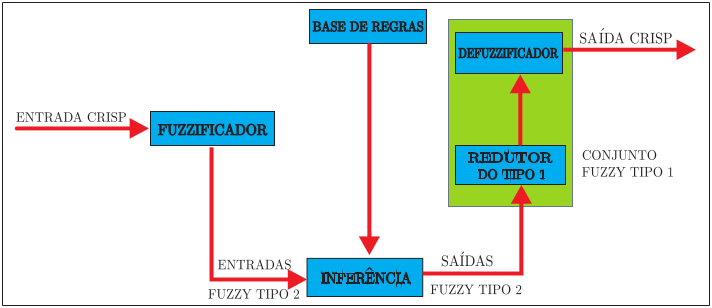
\includegraphics[scale=0.6]{images/sbrf2_dia_bloco.png}
\caption{Sistema Baseado em Regras Fuzzy 2.} %\citep{rizol2011logica}
\label{fig:sbrf2}
\end{figure}


\begin{itemize}
    \item [1] \textbf{Fuzzificador}: o bloco fuzzificador transforma o vetor de entrada $x^{'} = (x^{'}_{1},x^{'}_{2}, \dots , x^{'}_{I}), i = 1,2,\dots, I,$ do SBRF2 em conjuntos fuzzy do tipo 2;
    
    \item [2] \textbf{Base de Regras}: a base de regras do SBRF2 permanece a mesma forma do tipo 1. A diferença entre SBRF1 e SBRF2 está na natureza das funções de pertinência; 
    
    \textbf{Regra 1:} Se $((x_{1}$ é $\tilde{X}^{1}_{1})$ e $(x_{2}$ é $\tilde{X}^{1}_{2}))$ então $y$ é $Y^{1}$;
    
    \textbf{Regra 2:} Se $((x_{1}$ é $\tilde{X}^{2}_{1})$ e $(x_{2}$ é $\tilde{X}^{2}_{2}))$ então $y$ é $Y^{2}$;
    
    
    \item [3] \textbf{Inferência:} o bloco de inferência realiza o cálculo do SBRF2 com base nas regras fuzzy;
    
    \item [4] \textbf{Redutor do Tipo 1:} o bloco redutor do tipo 1 tem função de transformar T2FS em T1FS, ou seja, procura o melhor T1FS que representa o T2FS e que deve satisfazer a seguinte premissa: quando toda a incerteza desaparecer, o resultado do SBRF2 é reduzido em um SBRF1 \citep{mendel2001uncertain};
    
    \item [5] \textbf{Defuzzificador}: a saída defuzzificada do SBRF2 é dada pela média dos pontos limites $\underline{Y}$ e $\overline{Y}$, ou seja;
    \begin{equation}
	  Y_x_= \frac{\underline{Y}+\overline{Y}}{2} , \forall x \in \chi,
	\end{equation}
Os valores $\underline{Y}$ e $\overline{Y}$, podem ser calculados utilizando o método iterativo de Karnik e Mendel (algoritmo KM) \cite{rizol2011logica}.
Da mesma forma, o passo de defuzzificação pode ainda ser obtido através da utilização de um método convencional, tal como o centróide para obter o valor final da inferência.

	
\end{itemize}


\subsection{Ordens Admissíveis} \label{subsecOrdensAdmissiveis}

Além da abordagem de SBRF2 também considera-se o uso de uma ordem total para intervalos por meio das ordens admissíveis explicadas em \cite{bustince2013generation, zapata2017interval}, pois, por vezes, nem sempre uma lista de intervalos gerada com a saída do SBRF2 pode ser comparável através dos métodos convencionais. A seguir, as ordens admissíveis consideradas neste trabalho são relatadas:

\begin{Def} \label{DefOrdemXueYager}
Ordem de Xu e Yager~\cite{xu2006some}: $ \forall (X,Y) \in \mathbb{U}$, 

%\begin{small}
\begin{equation*}
[\underline{X}, \overline{X}] \leq_{XY} [\underline{Y}, \overline{Y}] \Leftrightarrow  
\left\{\begin{array}{l} \vspace{0.1cm}
\underline{X} + \overline{X} < \underline{Y} + \overline{Y};  \mbox{ou} \\ 
\underline{X} + \overline{X} = \underline{Y} + \overline{Y} ~\mbox{e}~ \overline{X} - \underline{X} \leq \overline{Y} - \underline{Y}.  \vspace{0.1cm}
\end{array}\right.
\end{equation*}
%\end{small}
\end{Def}


\begin{Def}
As Ordens Lexicográficas, $\leq_{Lex1}$ relacionada à primeira variável, e $\leq_{Lex2}$ correspondente a segunda variável, que são respectivamente definidas da seguinte forma:
  
\begin{align*}
[\underline{X}, \overline{X}] \leq_{Lex1} [\underline{Y}, \overline{Y}] & \Leftrightarrow \left\{\begin{array}{l} \vspace{0.1cm}
\underline{X} < \underline{Y}; \mbox{ou} \\ 
\underline{X} = \underline{Y} ~\mbox{e}~ \overline{X} \leq \underline{Y};
\vspace{0.1cm}
\end{array}\right.\\
[\underline{X}, \overline{X}] \leq_{Lex2} [\underline{Y}, \overline{Y}] & \Leftrightarrow \left\{\begin{array}{l} \vspace{0.1cm}
\overline{X} < \overline{Y}; \mbox{ou} \\ 
\overline{X} = \overline{Y} ~\mbox{e}~ \underline{X} \leq \underline{Y}.\hspace{2.0cm}
\vspace{0.1cm}
\end{array}\right.
\end{align*}

\end{Def}

\chapter{f-Cloud: Visão Geral e Modelagem}\label{sec:modelagem}

Este capítulo apresenta a concepção do sistema fuzzy para o fClouD bem como a proposta metodológica para sua aplicação em um simulador de CN.

\section{Tratamento de Incertezas na CN via Lógica Fuzzy Intervalar}

Esta seção apresenta a concepção, modelagem e prototipação do sistema fuzzy do fCloud, um módulo para auxiliar na tomada de decisão sobre as migrações de MVs em um ambiente de CN baseado em LF tipo-2, e caracterizado principalmente pela capacidade em lidar com as incertezas presentes nas variáveis do ambiente.

\subsection{Modelagem do Sistema Fuzzy para Tratamento das Incertezas}\label{secaomodelagem}

O fCloud foi desenvolvido para lidar com incertezas referentes a utilização de CPU, memória e rede nos computadores físicos presentes num ambiente de CN. Esta seção enfatiza os ganhos que o escalonador obteve com o auxílio do fCloud em situações as quais incertezas são presentes devido a oscilação nos valores das variáveis.

O fCloud considera que a disponibilidade dos valores de CPU, memória e rede são dadas por números fuzzy. O componente devolve ao escalonador uma lista de valores referentes ao nível de utilização de cada uma das máquinas físicas do ambiente.

Considera-se que os números fuzzy utilizam funções trapezoidais, para reproduzir situações em que o erro na medida extraída da grade pode ser tanto positiva como negativa. Assim, o poder computacional de um computador no ambiente é representado, utilizando a notação de números fuzzy, que representa a incerteza em torno do nível de utilização de processamento naquele momento.

De modo similar, para o valor de utilização da memória RAM de um computador no ambiente é representado, utilizando da notação de números fuzzy, que representa a incerteza em torno do nível de utilização da memória naquele momento. 

Também, a largura de banda disponível entre os computadores utiliza a notação de números fuzzy, que representa a incerteza em torno do nível de utilização da largura de banda naquele momento. 
 

\subsection{Base de Dados e Definição das Funções de Pertinência}

Antes de começar a trabalhar com as informações de entrada, fez-se necessário estudá-las juntamente com um especialista da área com a finalidade de determinar o comportamento do sistema a fim de obter valores de saída satisfatórios, de acordo com a necessidade do ambiente.

Nesta etapa, ocorre o processo de transformação de sentenças linguísticas em CFs. Também são determinados quantos e quais CF estão associados a cada variável do sistema. Ocorrendo desta forma, o processo de representação gráfico e análise funcional do comportamento das variáveis fuzzy, tanto de entrada como de saída.

Conforme a Figura~\ref{funcoes_pertinencia_modelagem}, neste projeto a modelagem dos CFs das variáveis são formadas por funções de pertinência trapezoidais, devido ao fato de representarem adequadamente o comportamento das variáveis dentro do T2FS.

Outra questão que também teve de ser estudada com o auxílio de especialistas, foi a definição dos pontos de intersecção entre os CFs de uma mesma variável. A intersecção destes conjuntos é essencial no desenvolvimento do sistema utilizando LF, com determinados valores de entrada mostrem pesos distintos em mais de um CF. Assim o sistema poderá aplicar a técnica de defuzzificação utilizada adequadamente para obtenção das saídas desejadas.

\begin{figure}[h]
	\centering
	%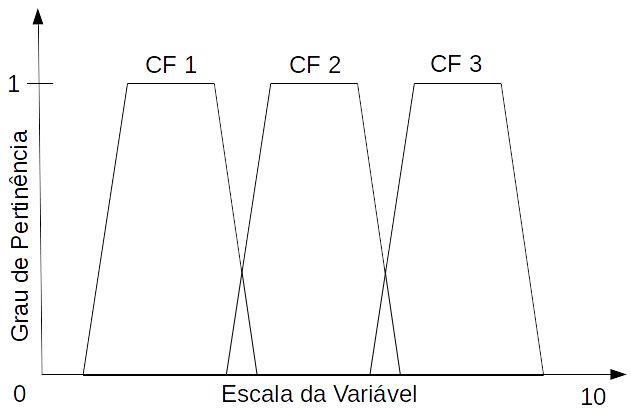
\includegraphics[width=0.5\textwidth]{images/funcoes_pertinencia_modelagem_trapmf.png}
	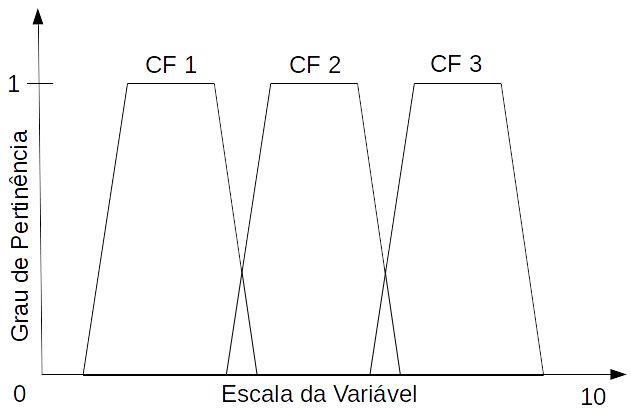
\includegraphics[scale=0.5]{images/funcoes_pertinencia_modelagem_trapmf.png}
	\caption{Modelo adotado para as Funções de Pertinência dos Conjuntos Fuzzy.}
	\label{funcoes_pertinencia_modelagem}
\end{figure}

%Outra questão que também teve de ser estudada com o auxílio de especialistas, foi definir os pontos de intersecção entre os CFs de uma mesma variável, conforme Figura \ref{funcoes_pertinencia_modelagem}, esses pontos de intersecção são essenciais no desenvolvimento do sistema utilizando LF, para que com determinados valores a entrada tenha peso em mais de um CF, assim o sistema poderá aplicar uma técnica de defuzzificação pertinente para obtenção das saídas desejadas.

O tratamento de incerteza e precisão utilizando a LF, foi possível dar maior robustez às informações obtidas, tornando a saída do escalonador mais confiável contribuindo para uma maior eficiência energética ao mesmo tempo mantendo desempenho.

Os processos executados pelo \emph{fCloud}, expostos no fluxograma da Figura \ref{processo_escalonamento_fuzzy}, representam a forma como ocorre a seleção dos recursos, na seguinte sequência: (i) na primeira etapa é realizada a coleta de informações sobre os recursos, (ii) depois estas informações são tratadas com uso da LF, que por fim (iii) é retornada uma lista com os valores referentes ao nível de utilização de cada máquina física do ambiente.

\newpage

\begin{figure}[h]
    \centering
    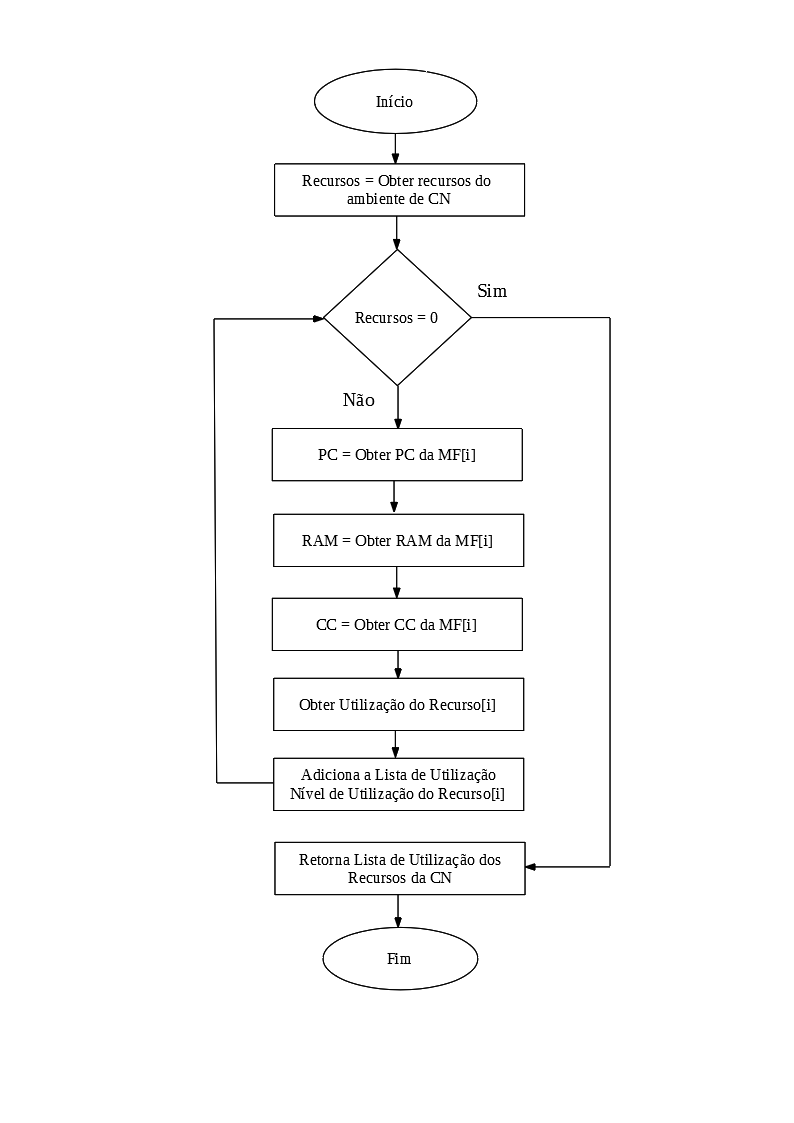
\includegraphics[scale=0.60]{images/startfigura29.png}
    \caption{Visão geral das funcionalidades do \emph{fCloud}.}
    \label{processo_escalonamento_fuzzy}
\end{figure}

Posteriormente, cabe ao escalonador realizar o mapeamento das MFs, determinando quais precisam que suas VMs sejam migradas e quais podem receber novas VMs, de acordo com os valores de utilização apresentados pelo fCloud.

Como os ambientes de CN possuem uma série de recursos a serem mensurados, este projeto focou em três recursos: Poder Computacional (PC), Memória RAM (RAM) e Custo Computacional (CC). Tais recursos são considerados relevantes nesse contexto e estão destacados na Figura \ref{modulo_fuzzy_modelagem}.

\begin{figure}[h]
    \centering
    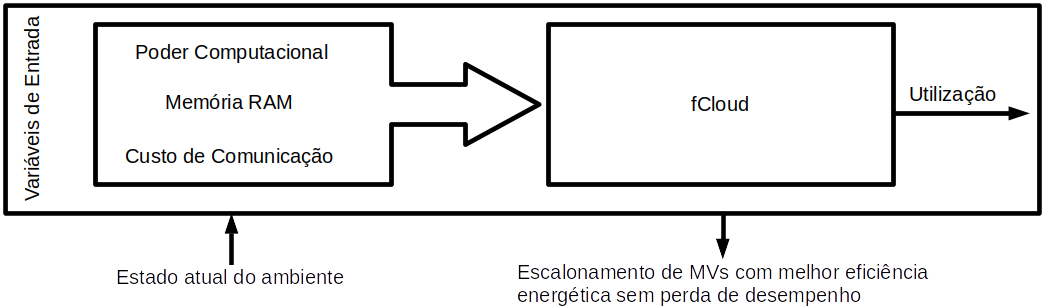
\includegraphics[scale=0.5]{images/modulo_fuzzy_modelagem.png}
   % 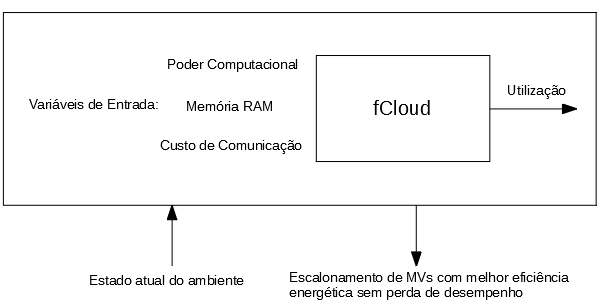
\includegraphics[scale=0.7]{images/cortadafigura29.PNG}
    \caption{Visão geral das entradas e saídas do \emph{fCloud}.}
    \label{modulo_fuzzy_modelagem}
\end{figure}

O \emph{fCloud} é responsável pela análise das MFs de um ambiente heterogêneo de CN e, para isso, faz o uso de um sistema fuzzy com uma base de regras atuando em três etapas: (i) Fuzzificação, (ii) Inferência e (iii) Defuzzificação e abrangendo um módulo especial de Redutor de Tipos. Este sistema retorna como saída o nível de utilização de cada máquina.

O estudo das variáveis teve como suporte as experiências do especialista em CN, as variáveis linguísticas relativas a cada uma das variáveis de incerteza foram transformadas em CFs, usando a representação gráfica trapezoidal para suas funções de pertinência. Na modelagem do sistema concedeu-se o emprego da ferramenta Juzzy~\cite{Juzzy2013}.

Para mensurar o PC, RAM e o CC é realizada a leitura das configurações do ambiente de CN simulado no CloudSim. Esses valores são então ajustados a uma escala padrão, considerando o intervalo $[0;10]$, e aplicando as equações:
%cpStandartScale = (_host.getMaxAvailableMips()/maxCPHost)*10;
\begin{eqnarray} 
 PC &=& (h_i(MM) / MaxPC * 10) \label{lblEqCPSS} \\
%ccStandartScale = (10*_host.getUtilizationOfBw())/minCCHost;
 CC &=& ((10 * h_i(UoB)) / MinCC) \label{lblEqCCSS} \\
%ramStandartScale = (_host.getUtilizationOfRam()/maxRamHost)*10;
 RAM &=& (h_i(UoR) / MaxRam) * 10  \label{lblEqRAMSS}
\end{eqnarray}

De acordo com os seguintes parâmetros:

\begin{itemize}
%\item $h_i$ representing the $host(i)$ of the cloud environment;
\item $h_i$ representando o $host(i)$ do ambiente da nuvem; 
%\item $MM$ as  Maximum MIPS available on host $i$ considering all processing elements (PE);
\item $MM$ as  Máximo de MIPS disponível no  host $i$ considerando todos os Processing Elements (PE);
%\item $UoB$ representing host $i$ bandwidth utilization;
\item $UoB$ representando a utilização de largura de banda do host $i$;
%\item $UoR$ as the host $i$ memory usage;
\item $UoR$ o uso de memória RAM no host $i$;
%\item $MaxCP$, as total value of the highest MIPS related to the best host in  the cloud environment;
\item $MaxPC$, valor total em MIPS do melhor host do ambiente da nuvem;
%\item $MinCC$ as the lowest communication cost in cloud environment;
\item $MinCC$ o menor custo de comunicação no ambiente da nuvem;
%\item $MaxRAM$ as the RAM capacity value of the best host.
\item $MaxRAM$ o valor de RAM do melhor host.
\end{itemize}

As equações (\ref{lblEqCPSS}), (\ref{lblEqCCSS}) e (\ref{lblEqRAMSS}) estão associadas as funções de pertinência das Figuras 16, 17, 18, complementando as variáveis PC, CC e RAM, respectivas.
Os Termos Linguísticos (TLs) definidos para os CFs da variável PC são: ``Limitado'' (PCL), ``Razoável'' (PCR) e ``Elevado'' (PCE - melhor caso). Sendo que para $PC = a$ e $a \in [0;10]$, têm-se as Funções de Pertinência da Tabela~\ref{lblTabMembershipPC}, as quais são graficamente descritas na Figura 16.

\begin{figure}[h]
%\vspace{-2mm}
\centering
%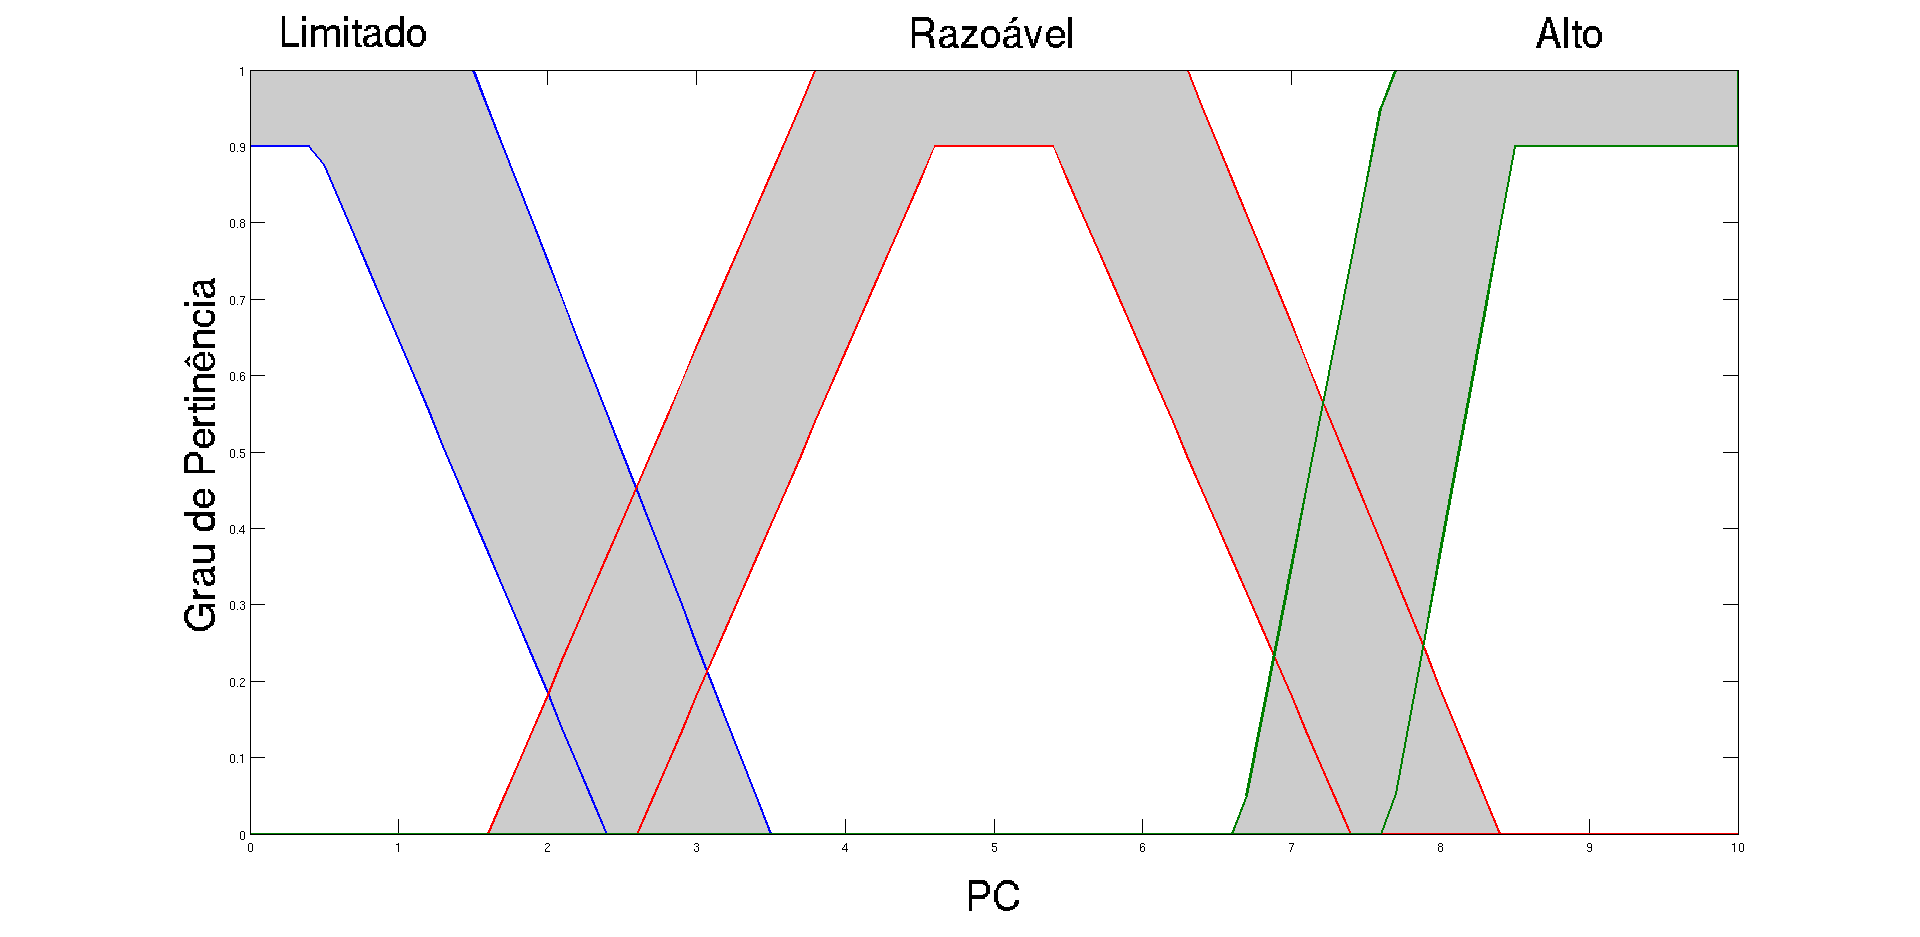
\includegraphics[scale=0.25]{images/Plot_PC.png}
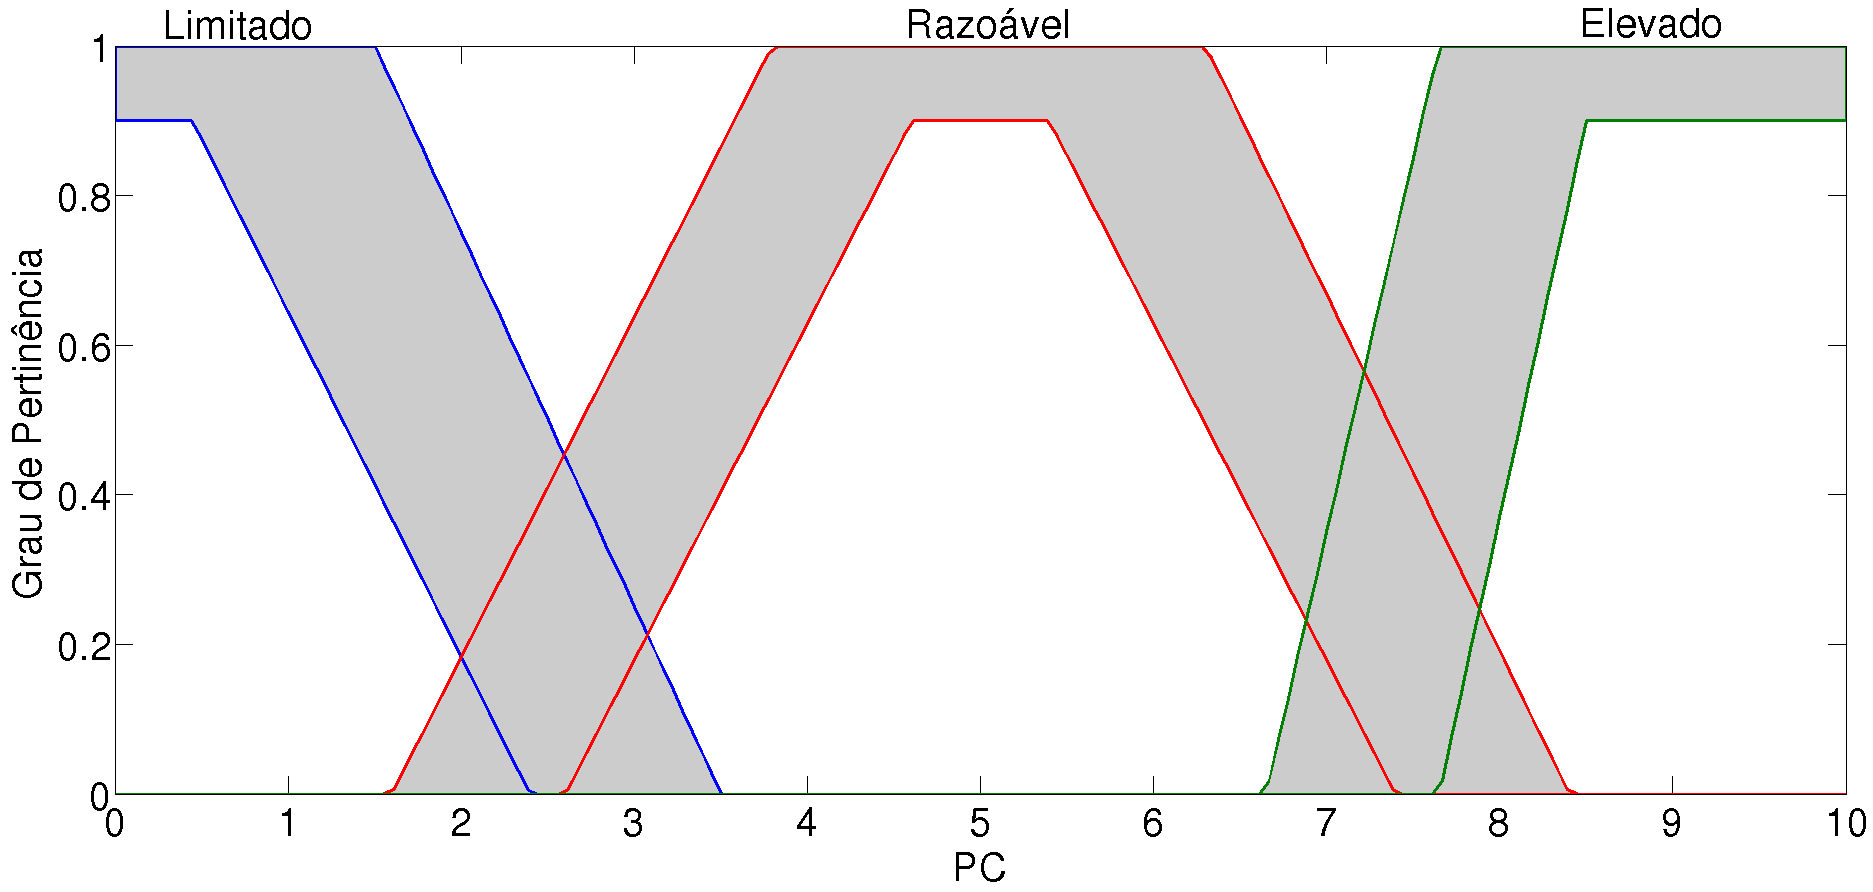
\includegraphics[scale=0.15]{images/Plot2_PC.png} %0.15
%p_membership_function2.png
%PR-Tipo2-TrapMF.png
%p_membership_function3.png Figura triangular a partir da deformação da trapezoidal
 \captionof{figure}{PC na escala padrão}
 \label{fig:PC_tipo1e2}
\end{figure}

\begin{table}[h]%[htp]
\scalefont{0.6} %0.6
\vspace{-4mm}
\begin{center}
\begin{tabular}{|c|l|l|} \hline 
PC &  $\overline{\mu_{A}(x)}$ & $\underline{\mu_{A(x)}}$  \\ \hline \hline
PCL & $\left\{\begin{array}{l} \vspace{0.2cm}
1, \mbox{~se~} \mbox{$0 \leq x < 1.5$} \\ 
\frac{-x+3.5}{2}, \mbox{~se~} \mbox{$1.5 \leq x < 3.5$}  \vspace{0.15cm} \\ 
0, \mbox{caso contrário.}  
\end{array}\right.$  & $\left\{\begin{array}{l} 
0.9, \mbox{~se~} \mbox{$0 \leq x < 0.45$} \vspace{0.15cm} \\
\frac{-0.9x + 2.4}{2.4}, \mbox{~se~} \mbox{$0.45 \leq x < 2.4$} \vspace{0.15cm} \\ 
0, \mbox{caso contrário.}  
\end{array}\right.$ \\ \hline 
 PCR &  $\left\{\begin{array}{l} \vspace{0.15cm}
\frac{x-1.6}{2.2}, \mbox{~se~} \mbox{$1.6 \leq x < 3.8,$} \vspace{0.1cm} \\ 
1, \mbox{~se~} \mbox{$3.8 \leq x < 6.3,$} \vspace{0.1cm}  \vspace{0.1cm}\\ 
\frac{-x+8.4}{2.1}, \mbox{~se~} \mbox{$6.3 \leq x < 8.4,$} \vspace{0.1cm}  \\ 
0, \mbox{caso contrário.}  
\end{array}\right.$ & $\left\{\begin{array}{l} \vspace{0.15cm}
0.45x-1,17, \mbox{~se~} \mbox{$2.6 \leq x < 4.6,$} \vspace{0.15cm} \\ 
%\frac{0.9x-2.6}{2}, \mbox{~se~} \mbox{$2.6 \leq x < 4.6,$} \vspace{0.15cm} \\ 
0.9, \mbox{~se~} \mbox{$4.6 \leq x < 5.4,$} \vspace{0.1cm}  \vspace{0.1cm}\\ 
%\frac{-0.9x+6.66}{2}, \mbox{~se~} \mbox{$5.4 \leq x < 7.4,$} \vspace{0.15cm}  \\ 
-0.45x+3.33, \mbox{~se~} \mbox{$5.4 \leq x < 7.4,$} \vspace{0.15cm} \\ 
0, \mbox{caso contrário.}  
\end{array}\right.$ \\ \hline
PCE & $\left\{\begin{array}{l} \vspace{0.15cm}
%\frac{x-6.65}{2}, \mbox{~se~} \mbox{$6.65 \leq x < 7.65,$} \vspace{0.1cm} \\
x-6.65, \mbox{~se~} \mbox{$6.65 \leq x < 7.65,$} \vspace{0.1cm} \\ 
1, \mbox{~se~} \mbox{$7.65 \leq x < 10,$} \vspace{0.1cm}  \\ 
0, \mbox{caso contrário.}  
\end{array}\right.$ & $\left\{\begin{array}{l} \vspace{0.1cm}
%\frac{0.9x-6.65}{1.5}, \mbox{~se~} \mbox{$7.8 \leq x < 8.5,$} \vspace{0.1cm} \\
\frac{18x}{17} - 8.1, \mbox{~se~} \mbox{$7.65 \leq x < 8.5,$} \vspace{0.1cm} \\ 
0.9, \mbox{~se~} \mbox{$8.5 \leq x < 10,$} \vspace{0.15cm} \\ 
0, \mbox{caso contrário.}  
\end{array}\right.$ \\ \hline
\end{tabular}
\end{center}
\caption{Funções de Pertinência PC}
\label{lblTabMembershipPC}
\end{table} 

\newpage

A variável RAM reporta-se, a porcentagem de utilização de memória RAM de uma máquina em determinado momento. Os TLs para os CFs definidos para essa variável são: ``Baixo'' (RAMB), ``Médio'' (RAMM) e ``Grande'' (RAMG - melhor caso). Sendo  que para $RAM = b$ e $b \in [0;10]$, têm-se as Funções de Pertinência da Tabela~\ref{lblTabMembershipRAM} que, graficamente estão descritas na Figura \ref{fig:RAM_tipo1e2}.


\begin{figure}[h]
%\vspace{-2mm}
\centering
%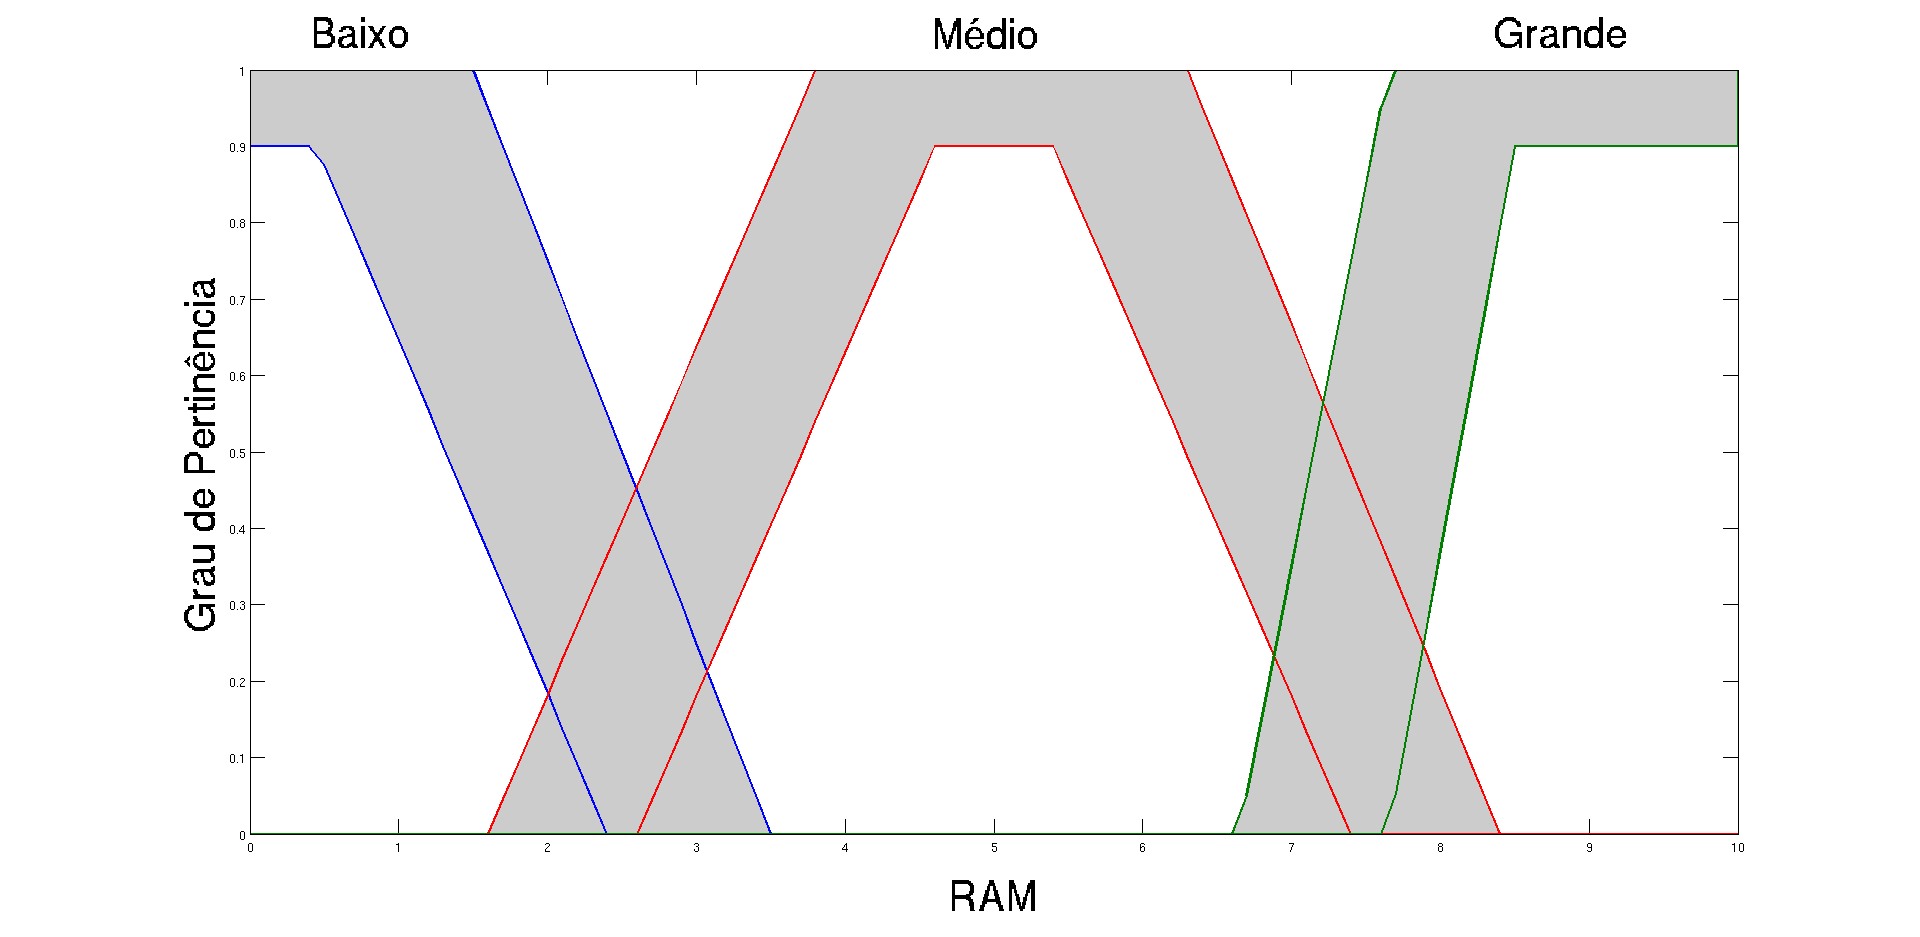
\includegraphics[scale=0.25]{images/Plot_RAM.png}
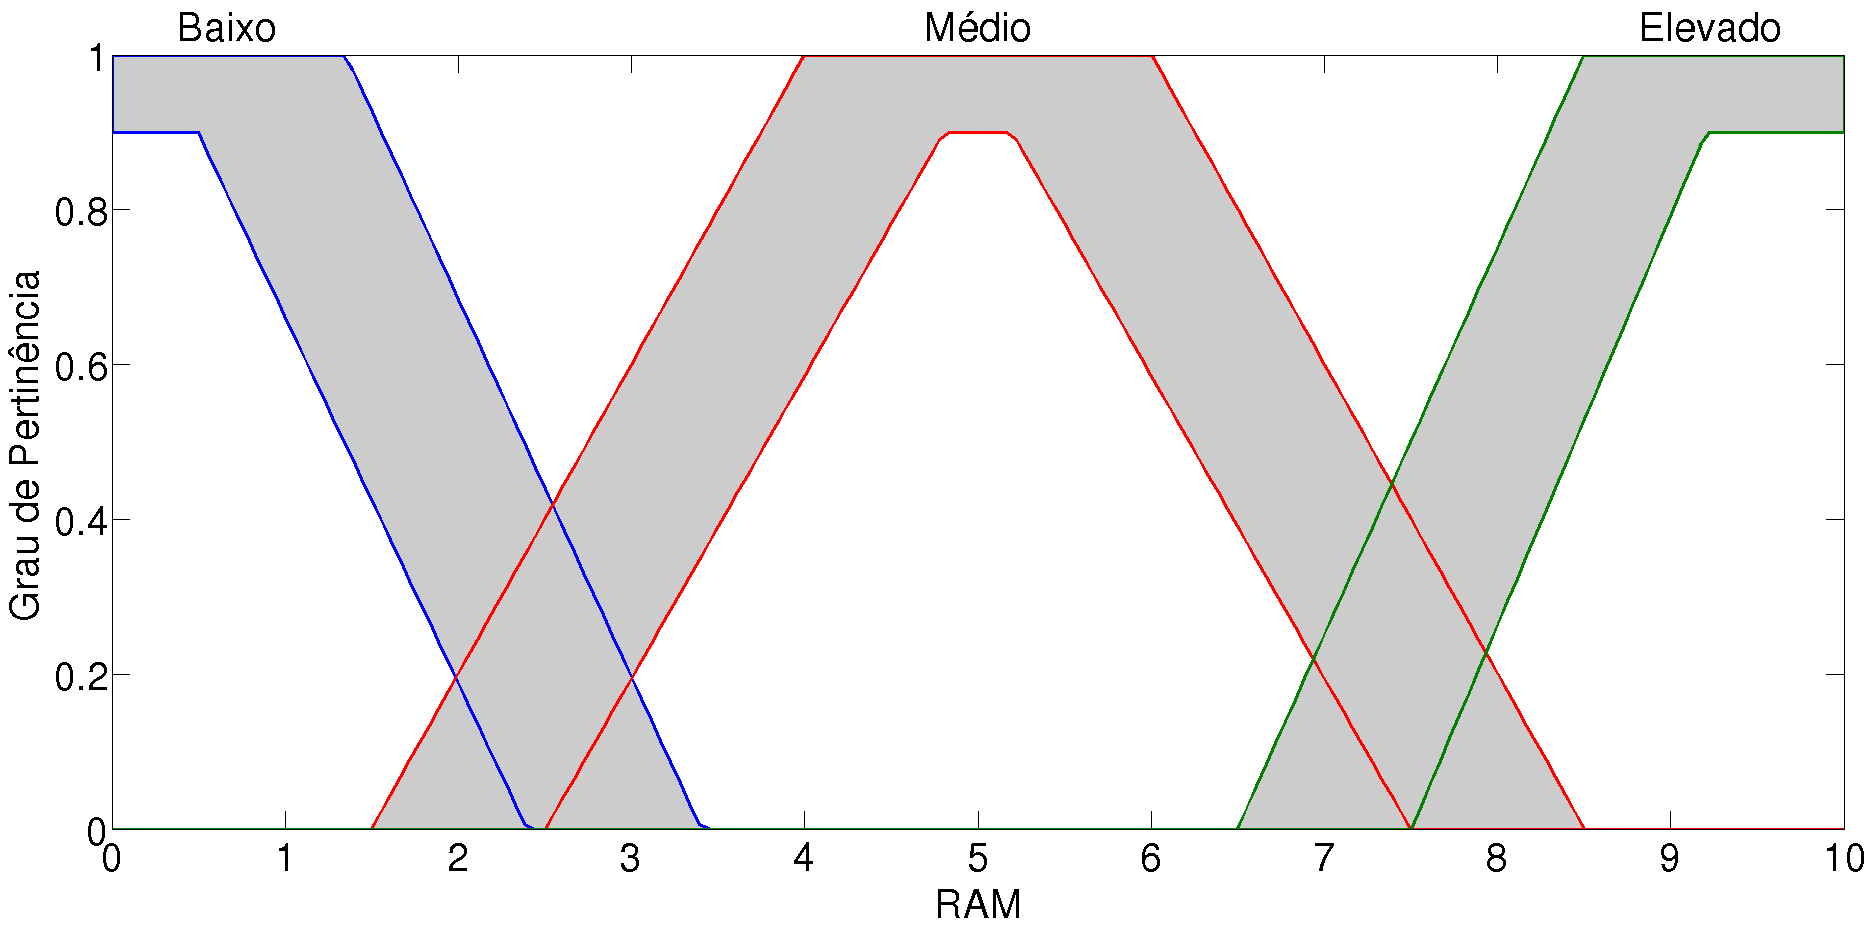
\includegraphics[scale=0.15]{images/Plot2_RAM.png}
%p_membership_function2.png
%PR-Tipo2-TrapMF.png
%p_membership_function3.png Figura triangular a partir da deformação da trapezoidal
 \captionof{figure}{RAM na escala padrão}
 \label{fig:RAM_tipo1e2}
\end{figure}

\begin{table}[h]%[htp]
\scalefont{0.6}
\vspace{-4mm}
\begin{center}
\begin{tabular}{|c|l|l|} \hline 
RAM &  $\overline{\mu_{A}(x)}$ & $\underline{\mu_{A(x)}}$  \\ \hline \hline
RAMB & $\left\{\begin{array}{l} \vspace{0.2cm}
1, \mbox{~se~} \mbox{$0 \leq x < 1.5$} \\ 
\frac{-x+3.5}{2}, \mbox{~se~} \mbox{$1.5 \leq x < 3.5$}  \vspace{0.15cm} \\ 
0, \mbox{caso contrário.}  
\end{array}\right.$  & $\left\{\begin{array}{l} 
0.9, \mbox{~se~} \mbox{$0 \leq x < 0.45$} \vspace{0.15cm} \\
\frac{-0.9x + 2.4}{2.4}, \mbox{~se~} \mbox{$0.45 \leq x < 2.4$} \vspace{0.15cm} \\ 
0, \mbox{caso contrário.}  
\end{array}\right.$ \\ \hline 
 RAMM &  $\left\{\begin{array}{l} \vspace{0.15cm}
\frac{x-1.6}{2.2}, \mbox{~se~} \mbox{$1.6 \leq x < 3.8,$} \vspace{0.1cm} \\ 
1, \mbox{~se~} \mbox{$3.8 \leq x < 6.3,$} \vspace{0.1cm}  \vspace{0.1cm}\\ 
\frac{-x+8.4}{2.1}, \mbox{~se~} \mbox{$6.3 \leq x < 8.4,$} \vspace{0.1cm}  \\ 
0, \mbox{caso contrário.}  
\end{array}\right.$ & $\left\{\begin{array}{l} \vspace{0.15cm}
0.45x-1,17, \mbox{~se~} \mbox{$2.6 \leq x < 4.6,$} \vspace{0.15cm} \\ 
%\frac{0.9x-2.6}{2}, \mbox{~se~} \mbox{$2.6 \leq x < 4.6,$} \vspace{0.15cm} \\ 
0.9, \mbox{~se~} \mbox{$4.6 \leq x < 5.4,$} \vspace{0.1cm}  \vspace{0.1cm}\\ 
%\frac{-0.9x+6.66}{2}, \mbox{~se~} \mbox{$5.4 \leq x < 7.4,$} \vspace{0.15cm}  \\ 
-0.45x+3.33, \mbox{~se~} \mbox{$5.4 \leq x < 7.4,$} \vspace{0.15cm} \\ 
0, \mbox{caso contrário.}  
\end{array}\right.$ \\ \hline
RAMG & $\left\{\begin{array}{l} \vspace{0.15cm}
%\frac{x-6.65}{2}, \mbox{~se~} \mbox{$6.65 \leq x < 7.65,$} \vspace{0.1cm} \\
x-6.65, \mbox{~se~} \mbox{$6.65 \leq x < 7.65,$} \vspace{0.1cm} \\ 
1, \mbox{~se~} \mbox{$7.65 \leq x < 10,$} \vspace{0.1cm}  \\ 
0, \mbox{caso contrário.}  
\end{array}\right.$ & $\left\{\begin{array}{l} \vspace{0.1cm}
%\frac{0.9x-6.65}{1.5}, \mbox{~se~} \mbox{$7.8 \leq x < 8.5,$} \vspace{0.1cm} \\
\frac{18x}{17} - 8.1, \mbox{~se~} \mbox{$7.65 \leq x < 8.5,$} \vspace{0.1cm} \\ 
0.9, \mbox{~se~} \mbox{$8.5 \leq x < 10,$} \vspace{0.15cm} \\ 
0, \mbox{caso contrário.}  
\end{array}\right.$ \\ \hline
\end{tabular}
\end{center}
\caption{Funções de Pertinência RAM}
\label{lblTabMembershipRAM}
\end{table} 

A variável CC reporta-se a porcentagem de utilização de banda da máquina sobre o máximo que essa suporta. Os TLs para os CFs definidos para essa variável são: ``Pequeno'' (CCP - melhor caso), ``Médio'' (CCM) e ``Grande'' (CCG). Sendo que para $CC = c$ e $c \in [0;10]$, têm-se as Funções de Pertinência da Tabela~\ref{lblTabMembershipCC2} que, estão descritas graficamente na Figura \ref{fig:CC_tipo1e2}. 

\begin{figure}[h]
%\vspace{-2mm}
\centering
%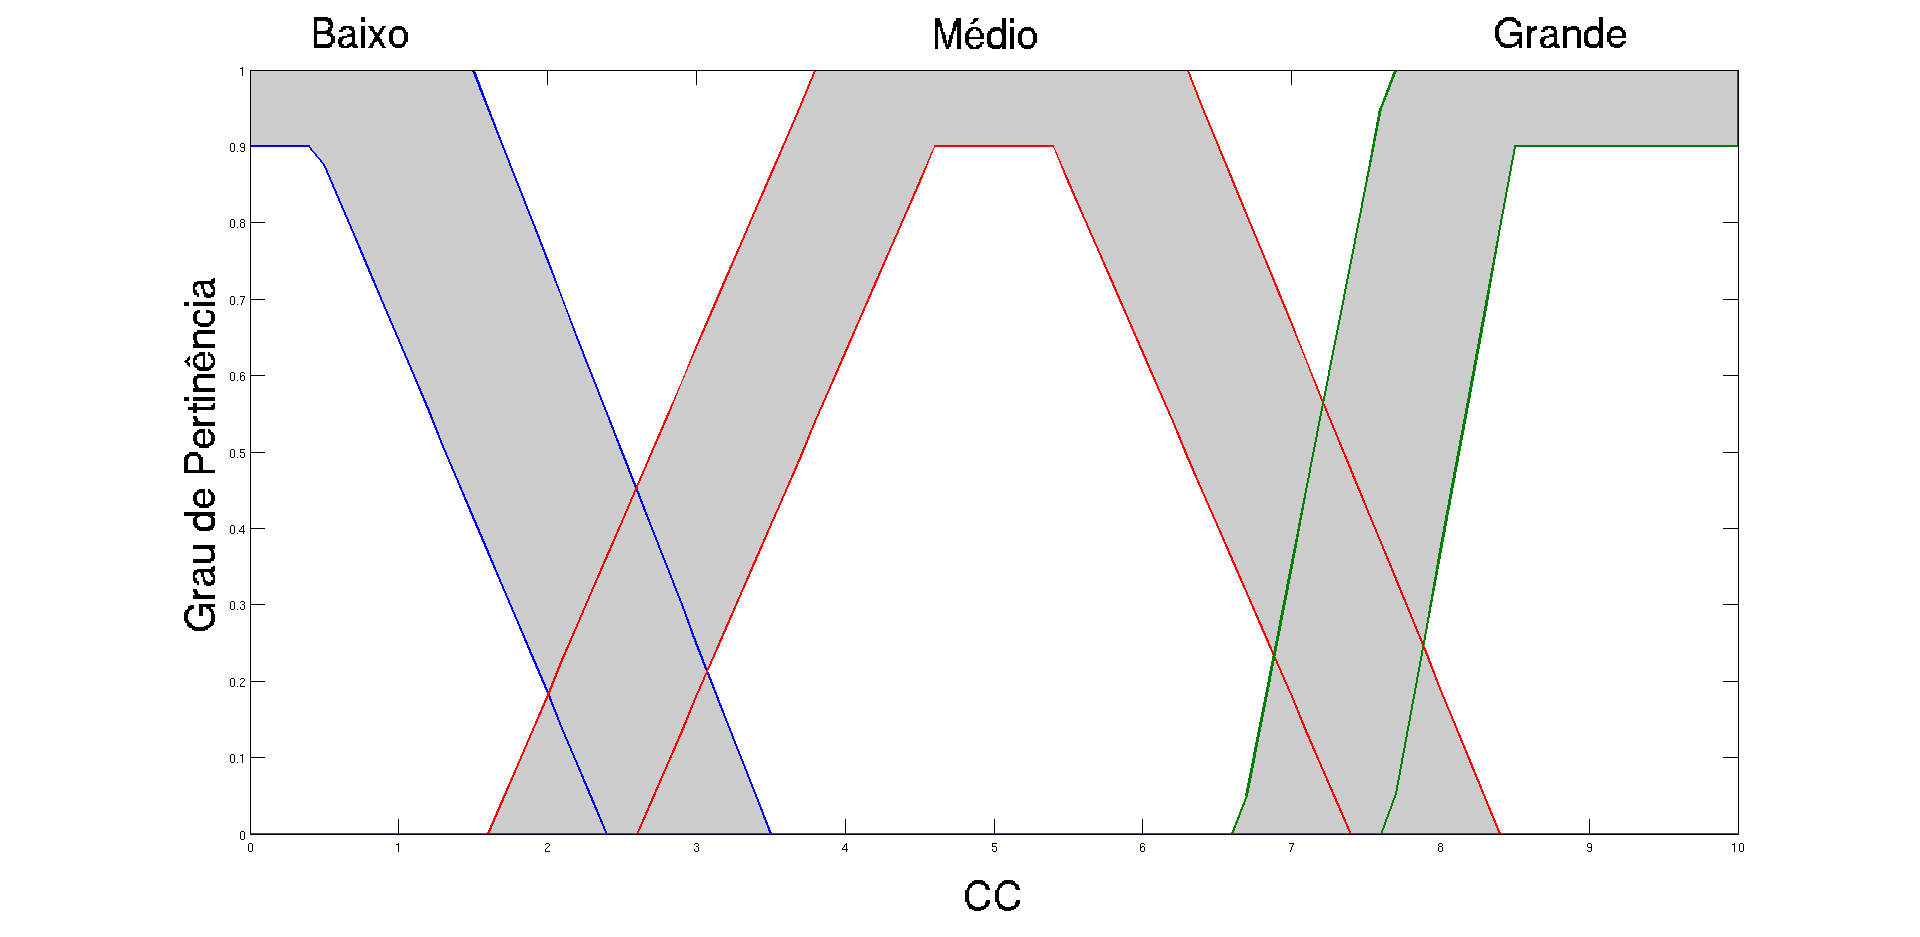
\includegraphics[scale=0.25]{images/Plot_CC.png}
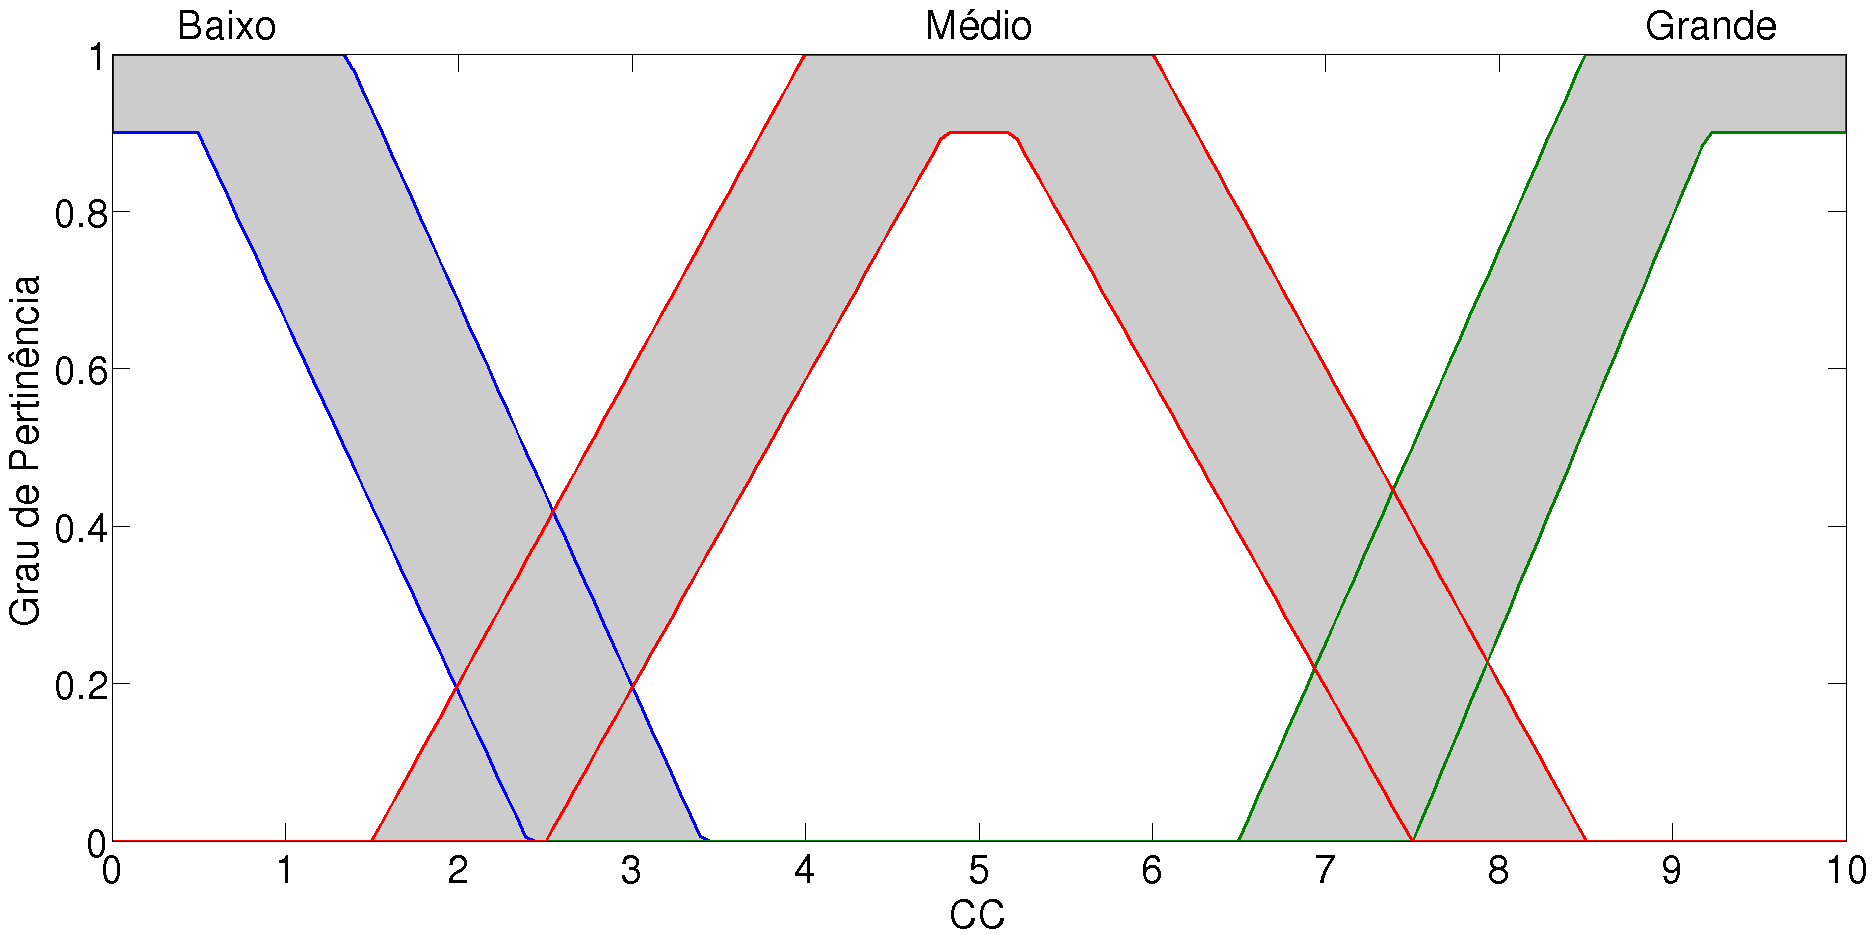
\includegraphics[scale=0.15]{images/Plot2_CC.png}
%cc_membership_function2.png
%CC-Tipo2-TrapMF.png
%img/cc_membership_function3.png Figura triangular apartir da deformação da trapezoidal
 \captionof{figure}{CC na escala padrão}
 \label{fig:CC_tipo1e2}
\end{figure}


\begin{table}[h]
%\vspace{-4mm}
\scalefont{0.6} % era .8
\begin{center}
\begin{tabular}{|r|l|l|} \hline 
CC & $\overline{\mu_{B}}_{\tilde{X}}$ & $\underline{\mu_{B}}_{\tilde{X}}$  \\ \hline \hline
CCP & $\left\{\begin{array}{l} \vspace{0.1cm}
1, \mbox{~se~} \mbox{$0 \leq x < 1.35,$} \vspace{0.1cm} \\ 
\frac{-x+3.4}{2.05}, \mbox{~se~} \mbox{$1.35 \leq x < 3.4,$} \vspace{0.1cm}  \\ 
0, \mbox{caso contrário.}  
\end{array}\right.$  & $\left\{\begin{array}{l} \vspace{0.1cm}
0.9, \mbox{~se~} \mbox{$0 \leq x < 0.5,$} \vspace{0.1cm} \\
\frac{-0.9x + 2.16}{1.9}, \mbox{~se~} \mbox{$0.5 \leq x < 2.4,$} \vspace{0.1cm} \\ 
0, \mbox{caso contrário.}  
\end{array}\right.$  \\ \hline
CCM & $\left\{\begin{array}{l} \vspace{0.1cm}
\frac{x-1.5}{2.5}, \mbox{~se~} \mbox{$1.5 \leq x < 2.5,$} \vspace{0.1cm}  \\ 
1, \mbox{~se~} \mbox{$4 \leq x < 6,$} \vspace{0.1cm} \\ 
\frac{-x+8.5}{2.5}, \mbox{~if~} \mbox{$6 \leq x < 8.5,$} \vspace{0.1cm}  \\ 
0, \mbox{caso contrário.}  
\end{array}\right.$ & $\left\{\begin{array}{l} \vspace{0.1cm}
%\frac{0.9x-2.18}{2.3}, \mbox{~se~} \mbox{$2.5 \leq x < 4.8,$} \vspace{0.1cm}  \\
\frac{0.9x-2.25}{2.3}, \mbox{~se~} \mbox{$2.5 \leq x < 4.8,$} \vspace{0.1cm}  \\ 
0,9, \mbox{~se~} \mbox{$4.8 \leq x < 5.2,$} \vspace{0.1cm} \\ 
\frac{-0.9x+6.75}{2.3}, \mbox{~se~} \mbox{$5.2 \leq x < 7.5,$} \vspace{0.1cm}  \\ 
0, \mbox{caso contrário.}  
\end{array}\right.$ \\ \hline
CCG & $\left\{\begin{array}{l} \vspace{0.1cm}
\frac{x - 6.5}{2}, \mbox{~se~} \mbox{$6.5 \leq x < 8.5,$} \vspace{0.1cm}  \\ 
1, \mbox{~se~} \mbox{$8.5 \leq x < 10,$} \vspace{0.1cm} \\ 
0, \mbox{caso contrário.}  
\end{array}\right.$ & $\left\{\begin{array}{l} \vspace{0.1cm}
%\frac{0.9x-6.5}{2}, \mbox{~se~} \mbox{$7.5 \leq x < 9.2,$} \vspace{0.1cm}  \\
\frac{18x-13.5}{3.4}, \mbox{~se~} \mbox{$7.5 \leq x < 9.2,$} \vspace{0.1cm}  \\ 
0.9, \mbox{~se~} \mbox{$9.2 \leq x < 10,$} \vspace{0.1cm} \\ 
0, \mbox{caso contrário.} 
\end{array}\right.$ \\ \hline
\end{tabular}
\end{center}
\caption{Funções de Pertinência CC}
\label{lblTabMembershipCC2}
\end{table}

\newpage

A saída U, que define o nível de utilização das máquinas em determinado momento, também é adaptada para uma escala padrão, conforme mostra a representação gráfica das correspondentes funções de pertinência na Figura~\ref{fig:mfutilizacao}. Os TLs para os CFs usados nesse caso são: ``Baixa'' (UB), ``Média'' (UM) e ``Alta'' (UA). Sendo $U = d$ e $d \in [0;10]$, têm-se as Funções de Pertinência da Tabela~\ref{lblTabMembershipPR2}.


\begin{figure}[h]
%\vspace{-2mm}
\centering
%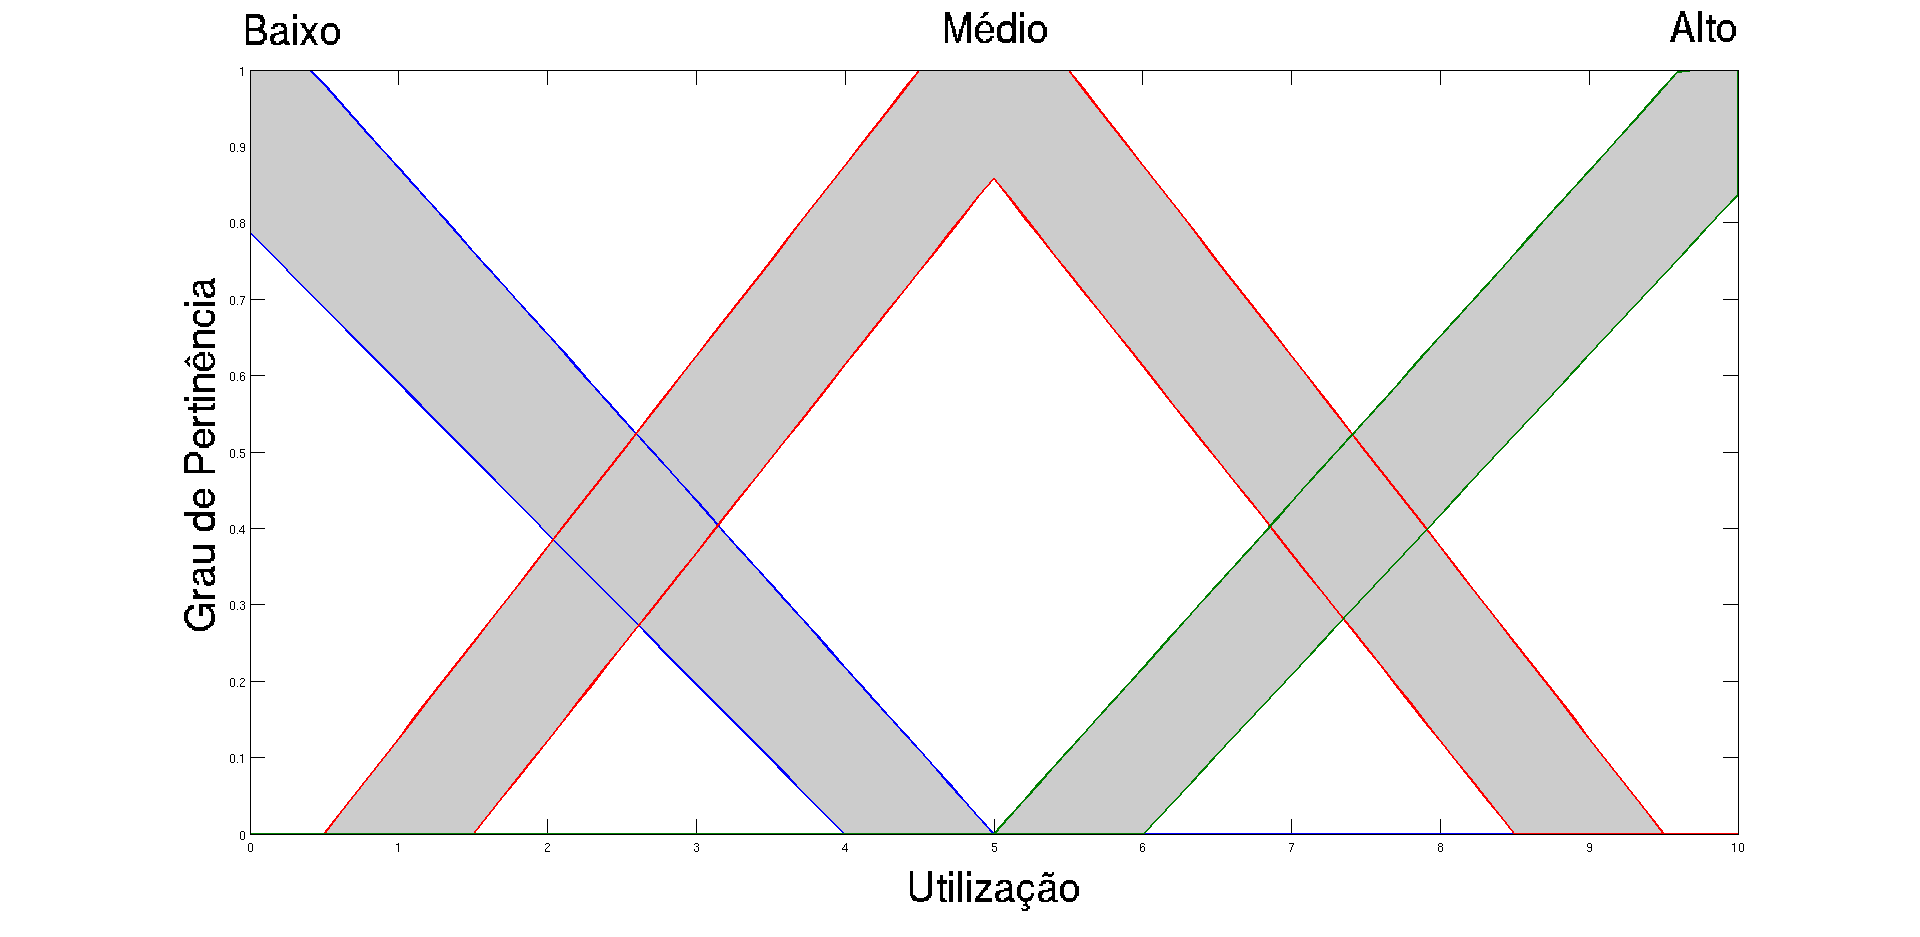
\includegraphics[scale=0.25]{images/Plot_Utilizacao.png}
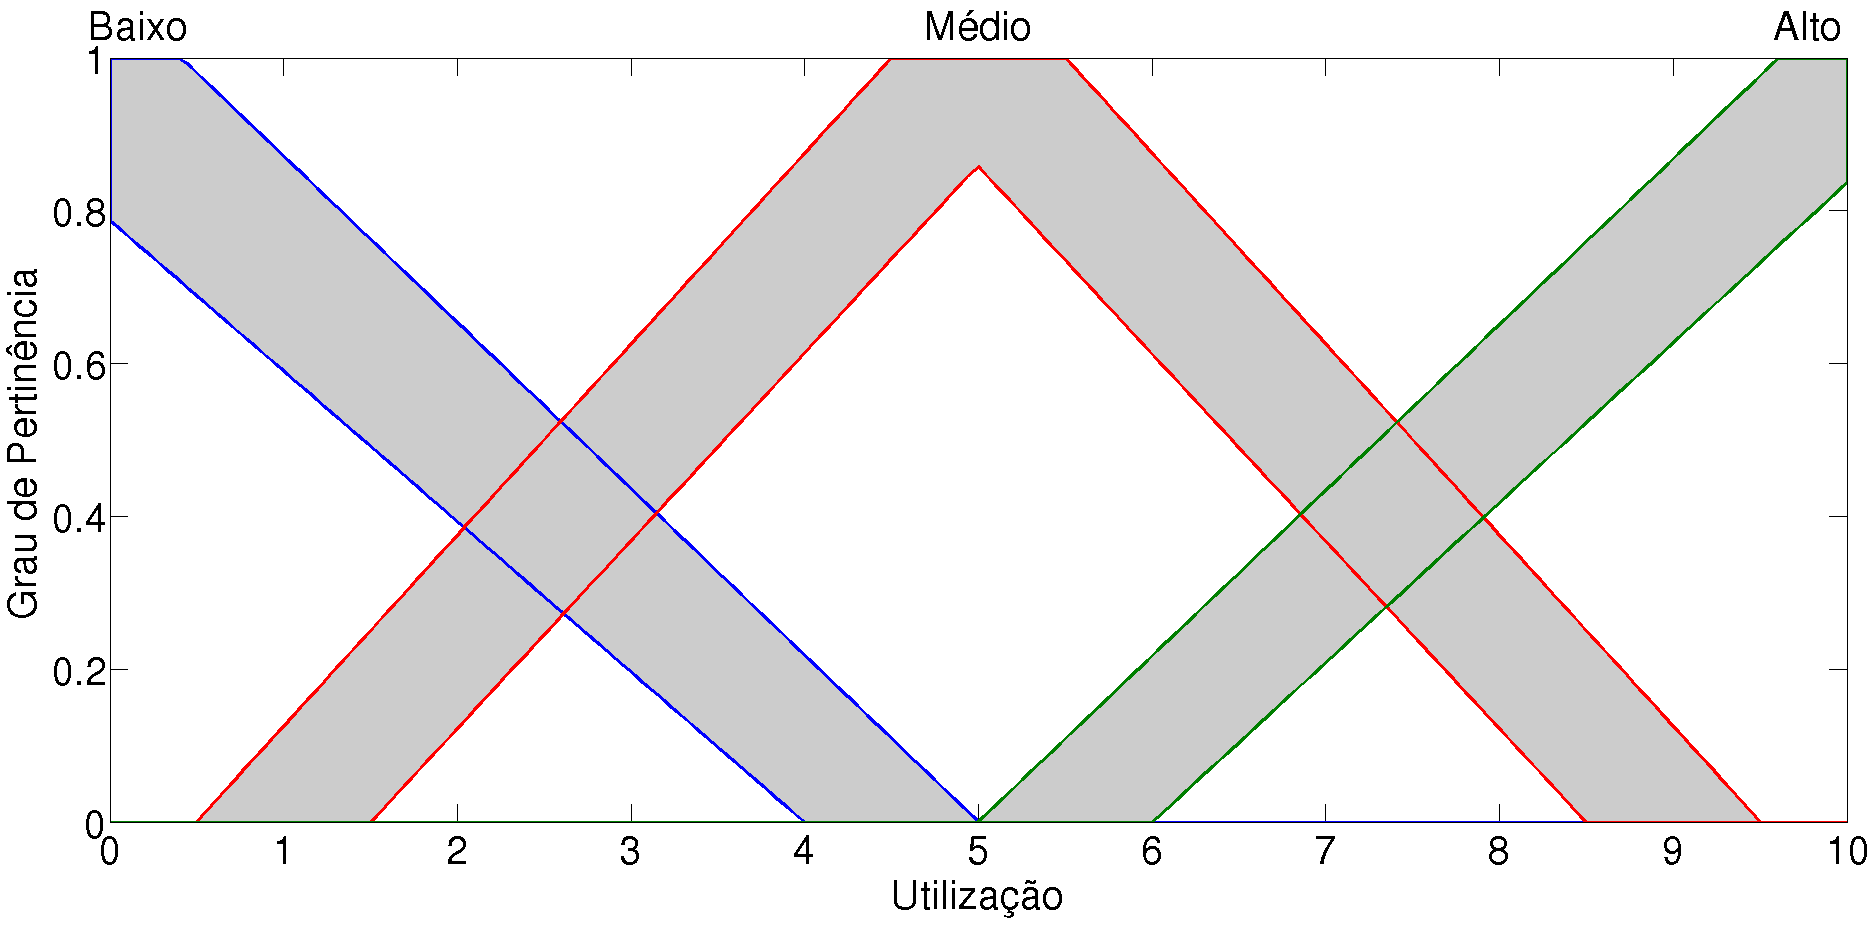
\includegraphics[scale=0.15]{images/Plot2_Utilizacao.png}
%p_membership_function2.png
%PR-Tipo2-TrapMF.png
%p_membership_function3.png Figura triangular a partir da deformação da trapezoidal
 \captionof{figure}{U na escala padrão}
 \label{fig:mfutilizacao}
\end{figure}


\begin{table}[h]
\scalefont{0.6}% era 0.8
%\vspace{-4mm}
\begin{center}
\begin{tabular}{|c|l|l|} \hline
U &  $\overline{\mu_{C}}_{\tilde{X}}$ & $\underline{\mu_{C}}_{\tilde{X}}$  \\ \hline \hline
UB & $\left\{\begin{array}{l} \vspace{0.1cm}
 \frac{x}{1,16}, \mbox{~se~} \mbox{$0 \leq x < 1.16,$} \\ 
1, \mbox{~se~} \mbox{$1.16 \leq x < 2.16,$} \vspace{0.1cm}  \\ 
%\frac{-x+3.5}{1.34}, \mbox{$2.16 \leq x < 5.5.$} \vspace{0.1cm} 
\frac{-x+3.5}{1.34}, \mbox{$2.16 \leq x < 3.5.$} \vspace{0.1cm} \\
0, \mbox{caso contrário.}  \vspace{0.1cm}
\end{array}\right.$  & $\left\{\begin{array}{l} \vspace{0.1cm}
\frac{0.9x-0.45}{1.333}, \mbox{~se~} \mbox{$0.5 \leq x < 1.66,$} \vspace{0.1cm} \\ 
\frac{-0.9x+2.52}{1.3}, \mbox{~se~} \mbox{$1.66 \leq x < 2.8,$} \vspace{0.1cm} \\ 
0, \mbox{caso contrário.}  \vspace{0.1cm}
\end{array}\right.$ \\ \hline 
UM &  $\left\{\begin{array}{l} \vspace{0.1cm}
%\frac{x-3.15}{2.01}, \mbox{~se~} \mbox{$3.15 \leq x < 5.16,$} \vspace{0.1cm} \\
\frac{-0.9x-3.447}{1.333}, \mbox{~se~} \mbox{$3.15 \leq x < 4.5,$} \vspace{0.1cm} \\ 
1, \mbox{~se~} \mbox{$4.5 \leq x < 5.5,$} \vspace{0.1cm}  \vspace{0.1cm}\\ 
\frac{-x+6.83}{1.327}, \mbox{~se~} \mbox{$5.5 \leq x < 6.83,$} \vspace{0.1cm}  \\ 
0, \mbox{caso contrário.}  \vspace{0.1cm}
\end{array}\right.$ & $\left\{\begin{array}{l} \vspace{0.1cm}
\frac{0.9x-3.447}{1.33}, \mbox{~se~} \mbox{$3.83 \leq x < 4.99,$} \vspace{0.1cm} \\ 
\frac{-0.9x+5.544}{1.12}, \mbox{~se~} \mbox{$4.99 \leq x < 6.16,$} \vspace{0.1cm}  \\ 
0, \mbox{caso contrário.} \vspace{0.1cm} \\ 
\end{array}\right.$ \\ \hline
UA & $\left\{\begin{array}{l} \vspace{0.1cm}
%\frac{x-6.65}{2}, \mbox{~se~} \mbox{$6.5 \leq x < 8.5,$} \vspace{0.1cm} \\
\frac{x-6.5}{1.33}, \mbox{~se~} \mbox{$6.5 \leq x < 7.83,$} \vspace{0.1cm} \\ 
1, \mbox{~se~} \mbox{$7.83 \leq x < 8.83,$} \vspace{0.1cm}  \\ 
\frac{-x+10}{1.17}, \mbox{~se~} \mbox{$8.83 \leq x < 10.$} \vspace{0.1cm} \\ 
0, \mbox{caso contrário.}  \vspace{0.1cm} \\
\end{array}\right.$ & $\left\{\begin{array}{l} \vspace{0.1cm}
\frac{0.9x-6.444}{1.34}, \mbox{~se~} \mbox{$7.16 \leq x < 8.33,$} \vspace{0.1cm} \\ 
\frac{-0.9x+8.55}{1.34}, \mbox{~se~} \mbox{$8.33 \leq x < 9.5,$} \vspace{0.1cm} \\ 
0, \mbox{caso contrário.} \vspace{0.1cm} \\ 
\end{array}\right.$ \\ \hline
\end{tabular}
\end{center}
\caption{Funções de Pertinência U}
\label{lblTabMembershipPR2}
\end{table} 

\newpage

\subsection{Fuzzificação}

Nessa etapa, ocorre o mapeamento dos valores de entrada (já ajustados para escala observada na Seção \ref{secaomodelagem}) para o domínio fuzzy, como pode ser observado na Figura \ref{fuzzificacaoModelagemPtBr}.

\begin{figure}[h]
   \centering
    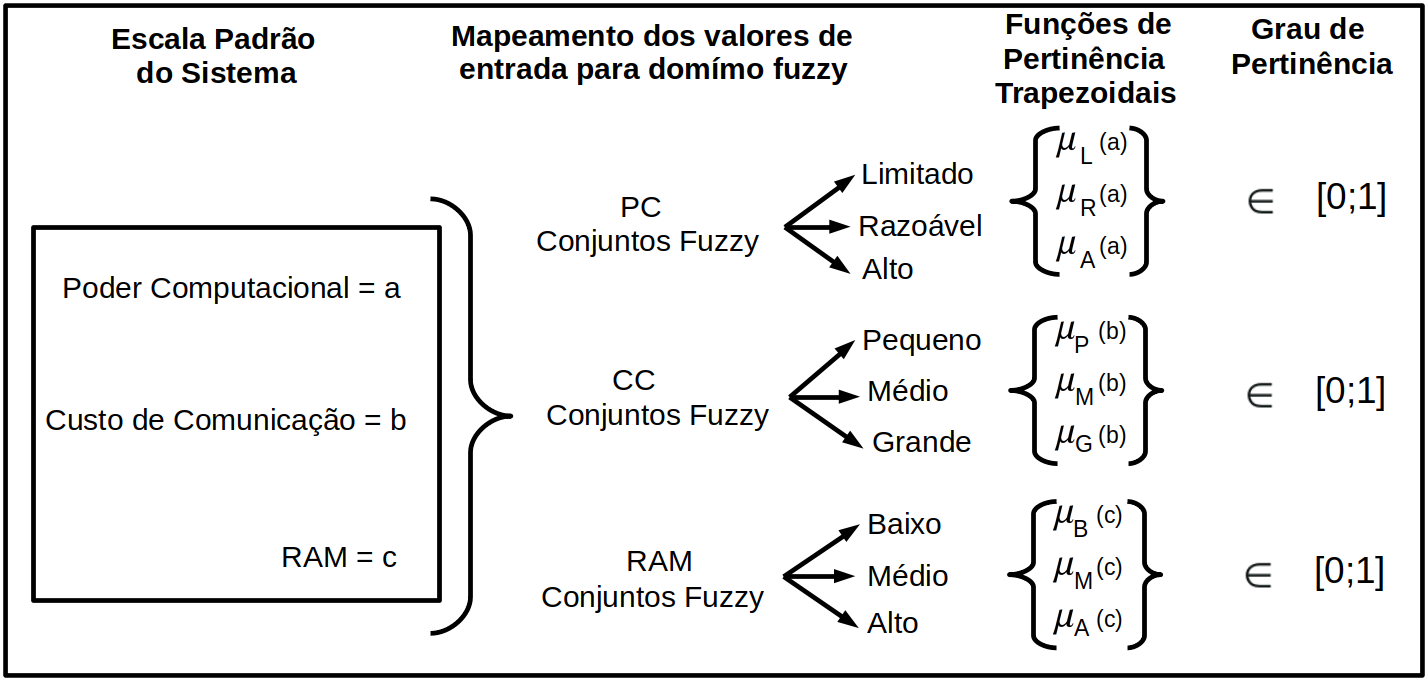
\includegraphics[scale = 0.4]{images/fuzzificacaoModelagemPtBr.png} %0.3
    \caption{Processo de Fuzzificação do fCloud}
    \label{fuzzificacaoModelagemPtBr}
\end{figure}

\subsection{Base de regras}\label{br}

A Base de Regras (BR) do \emph{fCloud} é desenvolvida com o intuito de ser facilmente compreensível e editável, visto que não há dificuldade em adicionar novas regras, caso seja desejado adicionar variáveis de entrada. A BR, observada na Tabela~\ref{lblBaseRegras}, leva em conta que o bom desempenho do sistema fuzzy está condicionado às regras que descrevem a estratégia de controle de forma consistente \cite{Klir2005}. Leva-se em conta três fatores para sua construção:

\begin{itemize}
	\item Modelando o sistema mais perto do \textbf{mundo real};
	\item São utilizadas conexões lógicas do tipo ``AND'' para criar a relação entre as variáveis de entrada;
	\item As implicações são do tipo $modus$ $ponens$ (modo afirmativo): \\ \begin{center}
	Se ((x é A) e (y é B) e (z é C)) então t é D.
	\end{center}
\end{itemize}

\begin{table}[h]
\centering
\caption{Base de Regras fCloud}
\scalefont{0.8}
\begin{tabular}{|c||l|l|l|l|}
\hline
\textbf{Regra} & \textbf{PC} & \textbf{CC} & \textbf{RAM} & \textbf{Utilização} \\ \hline \hline
1 &   limitado     &   pequeno   &   baixo     &  alto        \\ \hline
2 &   limitado    &   pequeno   &   médio   &  médio    \\ \hline
3 &   limitado    &   pequeno   &   alto       &  médio \\ \hline
4 &   limitado    &     médio    &   baixo      &  alto \\ \hline
5 &   limitado    &     médio    &   médio    & médio   \\ \hline
6 &   limitado   &      médio    &   alto      &  médio      \\ \hline
7 &   limitado     &        alto       &   baixo   &  alto   \\ \hline
8 &   limitado    &        alto       &   médio  &  alto    \\ \hline
9 &   limitado    &        alto       &   alto      &  alto    \\ \hline
10 &   razoável    &      baixo     &   baixo     &   médio  \\ \hline
11 &   razoável    &      baixo     &   médio   &   médio  \\ \hline
12 &   razoável    &      baixo     &   alto       &   médio  \\ \hline
13 &   razoável    &     médio    &   baixo     &   alto      \\ \hline
14 &   razoável    &     médio    &   médio   &   médio    \\ \hline
15 &   razoável     &     médio    &   alto       &   baixo    \\ \hline
16 &   razoável    &       alto      &   baixo     &   alto    \\ \hline
17 &   razoável     &       alto      &   médio   &   médio    \\ \hline
18 &   razoável     &       alto      &   alto       &   médio   \\ \hline
19 &      alto         &      baixo     &    baixo    &   médio    \\ \hline
20 &      alto         &      baixo     &   médio    &   baixo   \\ \hline
21 &      alto         &      baixo     &     alto      &   baixo   \\ \hline
22 &      alto         &     médio    &    baixo     &   médio    \\ \hline
23 &      alto         &     médio    &    médio   &   médio    \\ \hline
24 &      alto         &     médio    &      alto     &   médio    \\ \hline
25 &      alto         &       alto      &    baixo     &   alto    \\ \hline
26 &      alto         &       alto      &    médio   &   alto        \\ \hline
27 &      alto         &       alto      &      alto     &   médio  \\ \hline
\end{tabular}
\label{lblBaseRegras}
\end{table}

\newpage

\subsection{Inferência}\label{inf}

No processo de Inferência, ocorrem as operações entre os CFs, com combinação dos antecedentes das regras e  aplicação de implicações utilizando o operador \textit{modus ponens generalizado}. Este processo ocorre em três etapas detalhadas a seguir. 


\begin{description}
	\item [(i)] Aplicação da Operação Fuzzy: nesta etapa, ocorre a aplicação dos operadores fuzzy sendo que a entrada consta de três valores resultantes da fuzzificação. Como as regras são formadas pelo operador fuzzy ``AND'', a aplicação utiliza o método MIN (mínimo) sobre os dois valores retornados da fuzzificação;
	\item [(ii)] Aplicação do Método de Implicação Fuzzy: nesta etapa, é realizada uma combinação entre o valor obtido na aplicação do operador fuzzy e os valores do CF de saída da regra, utilizando o método IMP (implicação) sobre estas combinações;
	\item [(iii)] Aplicação do Método de Agregação Fuzzy: nesta etapa, ocorre a composição dos resultados fuzzy de saída de cada regra, utilizando o método MAX (máximo), assim criando uma única região fuzzy para ser analisada pelo próximo processo do módulo fuzzy.
\end{description}

\begin{figure}[h]
\centering
%\includegraphics[width=.9\textwidth]{InferenciaModelagem2.jpg}
%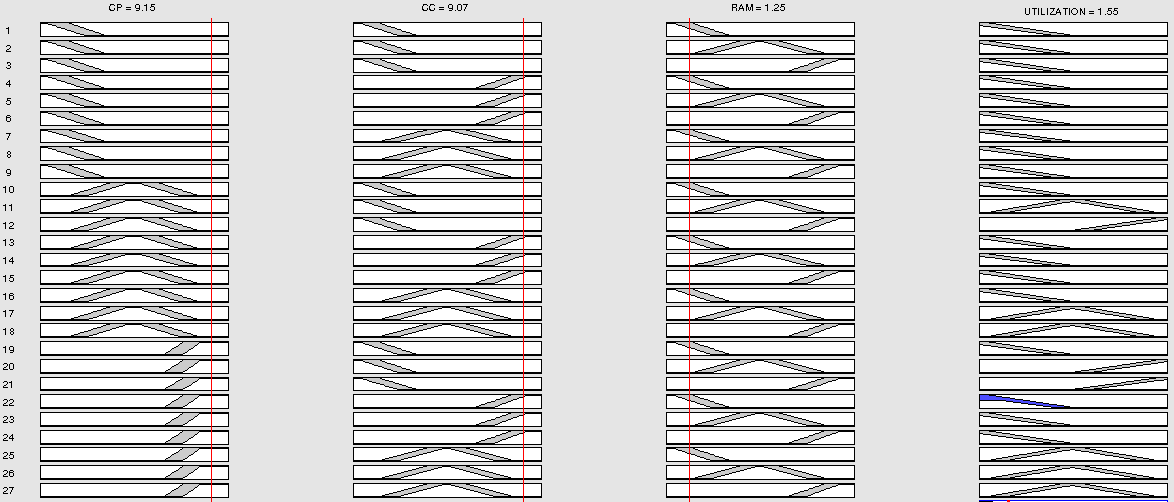
\includegraphics[scale=0.3]{images/inferencia.png}
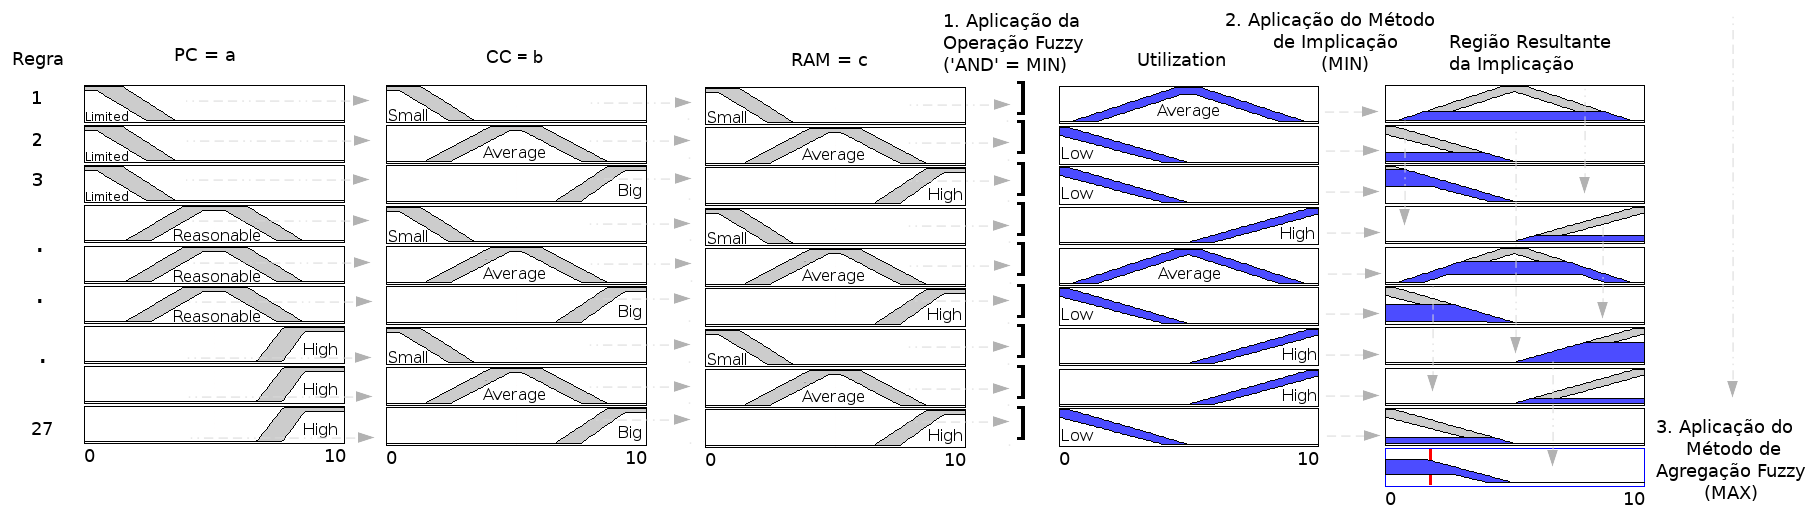
\includegraphics[scale=0.23]{images/InferenciaModelagemFuzzIeee2019PtBr.png}
%img/InferenciaModelagem4.png %InferenciaModelagem5.png
\caption{Processo de Inferência do fCloud}
\label{fig:infe2}
\end{figure}

\subsection{Defuzzificação}

Nessa etapa, ocorre a transformação da região resultado da Inferência em um valor discreto que representa a Utilização (U). Essa transformação foi feita no \emph{fCloud} através do emprego do método centro da área. Esse método calcula o centroide (x) da área composta pela saída fuzzy do sistema de Inferência, o qual considera a união de todas as contribuições de regras descutidas nas seções \ref{br} e \ref{inf}. A expressão analítico da centroide é dada pela equação
%calculado através da fórmula da Equação (\ref{lblEqCentroideSF2}).
\begin{equation} \label{lblEqCentroideSF2}
  u=  \frac{ \sum _{i=1} ^N u_i \mu_{OUT}(u_i) }{  \sum _{i=1} ^N \mu_{OUT}(u_i)  } \\
\end{equation}

\newpage

\section{Visão Geral dos Procedimentos Operacionais do fCloud}

Nesta seção, a visão geral dos procedimentos relacionados à operação do fCloud é discutida, apresentando de  de forma integrada todas as etapas descritas na Seção~\ref{sec:modelagem}.

\begin{figure}[h]
\centering
%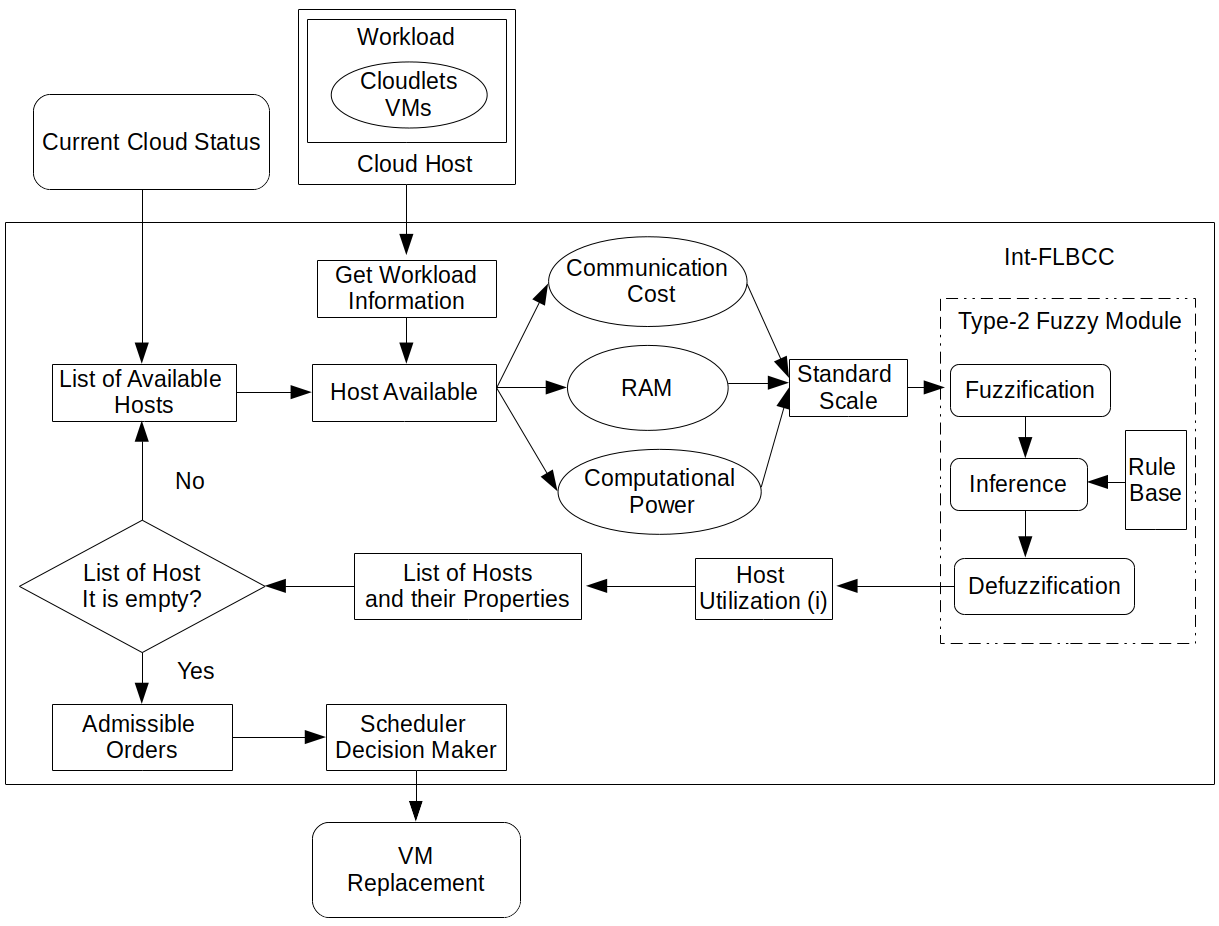
\includegraphics[scale=0.5]{images/flowchart_intflbcc.png} %Fluxograma_do_Modulo_Fuzzy.jpg
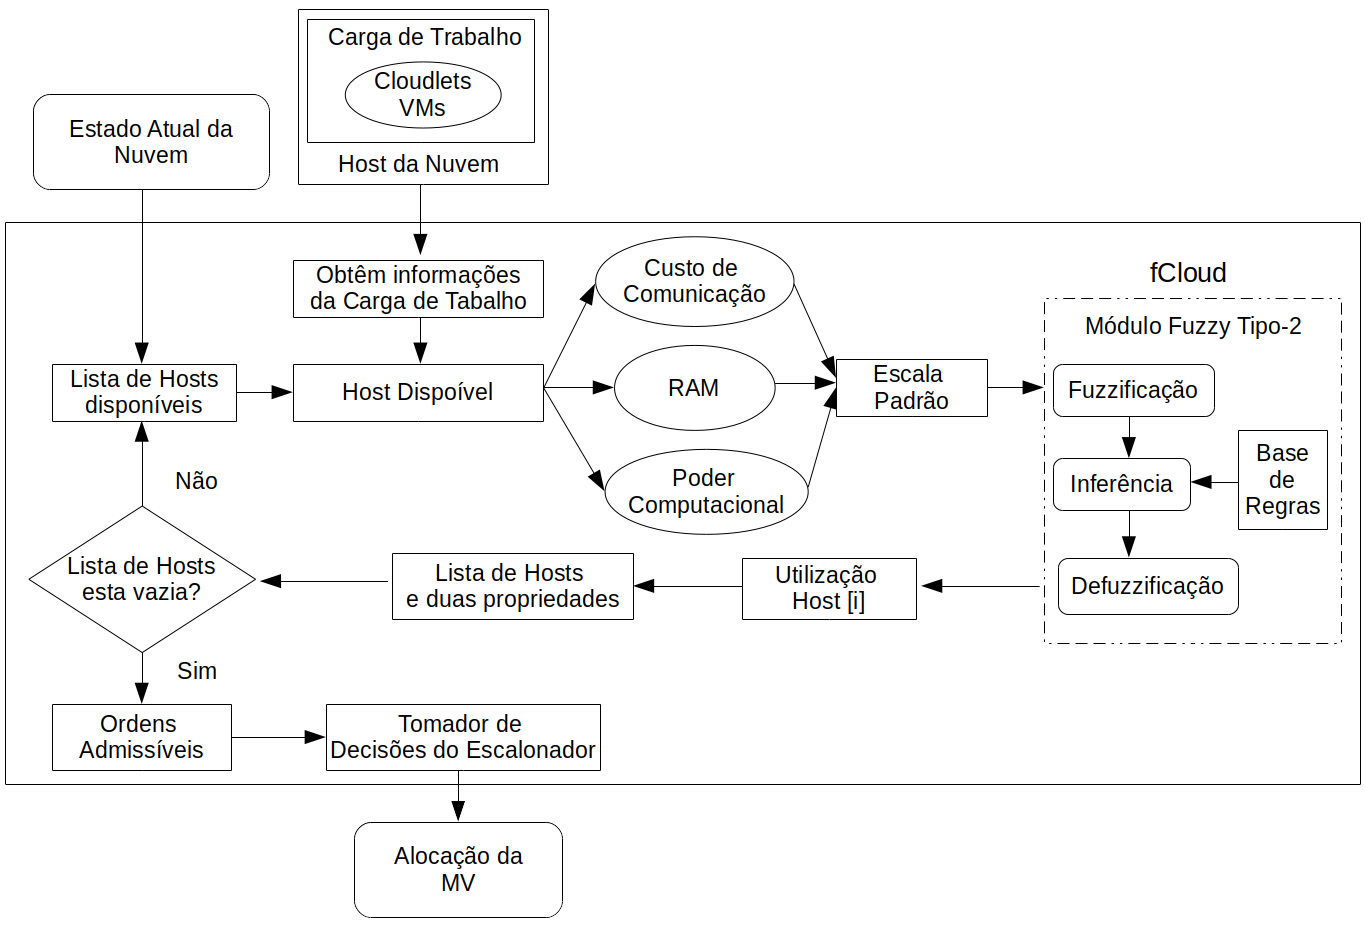
\includegraphics[scale=0.45]{images/fluxograma_int_flbcc_ptbr.png} 
\caption{Fluxograma dos processos operacionais do fCloud.}
\label{Fluxograma_fCloud}
\end{figure}

A visão geral dos processos envolvidos na operação do \emph{fCloud} é descrita pelo fluxograma apresentado na Figura~\ref{Fluxograma_fCloud}. O mesmo recebe como entrada o estado atual dos recursos da nuvem computacional, e a carga de trabalho a ser atribuída  ao ambiente da nuvem.

Na sequência duas variáveis são identificadas (i) o estado atual do ambiente da CN; (ii) as máquinas que estão disponíveis, sendo ambas armazenadas em uma lista. A seguir são coletadas as informações de CC, RAM e PC de cada máquina disponível, adaptando-os para uma Escala Padrão, onde estarão prontas para ingressarem no Módulo Fuzzy Tipo-2. O módulo fuzzy tem a composição de três etapas: (i) Fuzzificacão, (ii) Inferência e (iii) Defuzzificação,  desta forma obtendo o intervalo correspondente ao nível de utilização de cada máquina disponível, armazenando estes em uma Lista de Níveis de Utilização, e após é verificado se ainda há alguma máquina disponível não analisada. Enquanto houver, analisa os dados e armazena na lista de Níveis de Utilização. Assim obtêm-se a lista contendo os intervalos de nível de uso de cada host do ambiente da CN.
A seguir, a Lista de Níveis de Utilização entra na etapa de ordenação, onde são aplicados os métodos das Ordens Admissíveis: (i) Lex1; (ii) Lex2 e (iii) Xu and Yager descritas na Seção \ref{subsecOrdensAdmissiveis}. Neste caso, têm-se uma solução para o problema de incompatibilidade dos intervalos no procedimento. Nem sempre uma lista de intervalos pode ser ordenada por métodos convencionais (ordenação usual dos intervalos reais).
Esta lista é enviada ao Tomador de Decisões do Escalonador que, por sua vez, irá mapear quais os hosts que devem ter MVs realocadas, e quais podem receber MVs, isto ocorre de acordo com os níveis de utilização e o método de ordenação selecionado. Onde máquinas com valores de utilização muito baixo podem ter suas MVs realocadas, e serem desligadas, visando um menor consumo energético. 
No caso das máquinas com valores de utilização muito alto, poderá ocorrer a realocação de suas MVs na tentativa de evitar perda de desempenho do ambiente. Desta forma, as máquinas disponíveis, que estiverem entre esses dois casos, serão as primeiras a receberem MVs.

\chapter{f-Cloud: Análise de Desempenho} \label{capAnaliseDeDesempenho}

Este capítulo apresenta as avaliações realizadas durante o andamento do projeto. Os níveis de utilização dos recursos obtidos através do emprego do módulo fCloud com SBRF2 foram aplicados na tomada de decisão quando da realização do escalonamento de MVs em um ambiente simulado de CN.

\section{Configuração do ambiente}
As avaliações empregaram, nesta pesquisa, simulações realizadas com uso das funcionalidades do framework CloudSim~\cite{calheiros2011cloudsim}, um kit de ferramentas para modelagem e simulação de serviços de CN. Na escolha do ambiente, considerou-se compatibilidade de código, suporte a T2FL e abordagem \emph{open-source} das bibliotecas

Na implementação do sistema de inferência fuzzy do f-ClouD foi utilizada a biblioteca Java de código aberto Juzzy \cite{Juzzy2013}, devido a seu potencial na manipulação de SBRF2, e ainda, por ser concebida em Java, mesma linguagem que o CloudSim foi desenvolvido. O uso de tecnologias compatíveis viabilizou a integração entre o ambiente simulado de CN, e o sistema de inferência fuzzy.

Para todas as simulações, considerou-se também as cargas de trabalho do mundo real fornecidas como parte do projeto CoMon \cite{CoMon2006}, uma infraestrutura de monitoramento para o PlanetLab \cite{chun2003planetlab}. O ambiente de nuvem IaaS, aplicado para os testes, considerou um \textit{data center} de grande escala com 800 hosts físicos heterogêneos, contemplando dois tipos de configurações, como descritas na Tabela \ref{lblConfAmbiente}.

\begin{table}[h]
\centering
\scalefont{0.8}
\begin{tabular}{|p{1.7cm}||p{3.5cm}|p{2.8cm}|p{2.8cm}|p{2cm}|} \hline
\textbf{Fabricante} & \textbf{Modelo} & \textbf{Nome do CPU} & \textbf{Características de CPU} & \textbf{RAM (GB)} \\ \hline \hline
Hewlett Packard Enterprise & ProLiant DL325 Gen10 & AMD EPYC 7551P 2.0 GHz & 32-Core, 2.0 GHz, 64MB L3 Cache &  128 \\ \hline
Dell Inc. & PowerEdge R840 (Intel Xeon Platinum 8180 2.50 GHz) & Intel Xeon Platinum 8180 2.50 GHz & 28 core, 2.50 GHz, 38.5 MB L3 Cache & 384 \\ \hline
\end{tabular}
\caption{Características dos hosts do ambiente da nuvem}
\label{lblConfAmbiente}
\end{table}

\newpage

Na Figura \ref{Caracteriscas_Cloud}, são apresentadas as características consideradas na arquitetura de nuvem computacional simulada.

\begin{figure}[h]
\centering
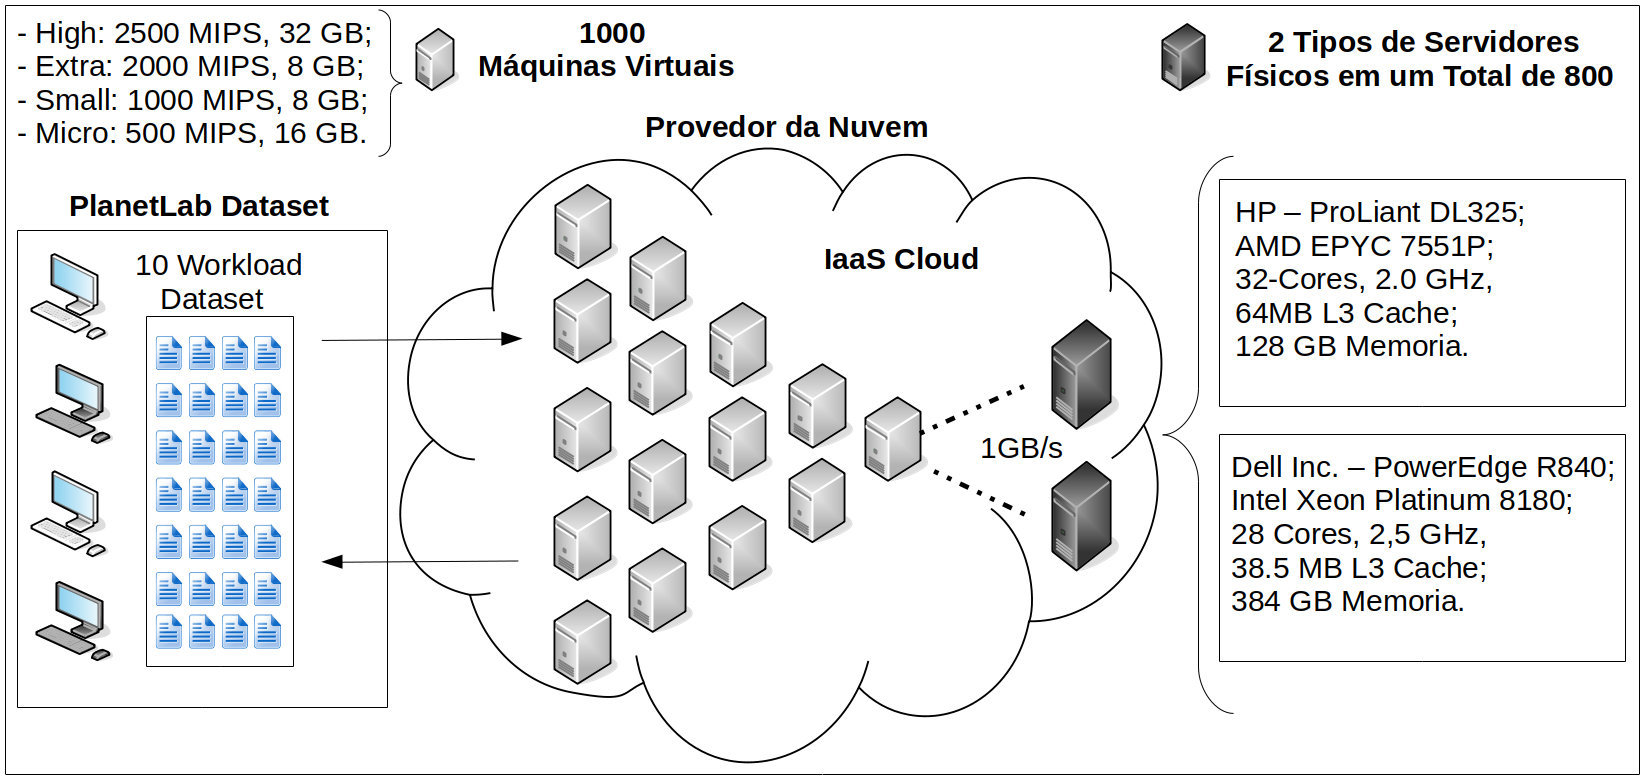
\includegraphics[scale=0.4]{images/caracteriscas_cloud_ptbr2.png} 
\caption{Características da Arquitetura da Nuvem Simulada.}
\label{Caracteriscas_Cloud}
\end{figure}


A frequência das CPUs do servidor é descrita em MIPS. Metade dos hosts são ProLiant DL325 Gen 10 com 4721 MIPS para cada núcleo, e a outra metade consiste no servidor PowerEdge R840 com 4520 MIPS para cada núcleo. Cada servidor é modelado para ter 5 GB/s de largura de banda de rede. 
As características dos tipos de MV são semelhantes aos tipos de instância do Amazon EC2 \cite{amazon2015amazon}, incluindo Instância de CPU Média Alta (4000 MIPS, 32 GB); Instância Extra Grande (3000 MIPS, 8 GB); Instância Pequena (2000 MIPS, 8 GB); e Micro Instância (2000 MIPS, 16 GB). 
O intervalo de medição de uso (intervalo de escalonamento) é de 5 minutos. As características de cada carga de trabalho são mostradas na Tabela \ref{lblConfCloudlets}. %Como mencionado em \cite{Barroso2007}, os valores de carga de trabalho confirmam que a utilização média de CPU é bem abaixo de 50\%.

\begin{table}[htbp]
\scalefont{0.8}
\begin{center}
\begin{tabular}{|r||r|r|r|} \hline
\textbf{Carga de Trabalho} &  \textbf{VMs} & \textbf{Média} (\%) & \textbf{Desvio Padrão} (\%) \\ \hline 
20110303 & 1052 & 12,31 & 17,09 \\ \hline
20110306 & 898 & 11,44 & 16,83 \\ \hline
20110309 & 1061 & 10,7 & 15,57 \\ \hline
20110322 & 1516 & 9,26 & 12,78 \\ \hline
20110325 & 1078 & 10,56 & 14,14 \\ \hline
20110403 & 1463 & 12,39 & 16,55 \\ \hline
20110409 & 1358 & 11,12 & 15,09 \\ \hline
20110411 & 1233 & 11,56 & 15,07 \\ \hline
20110412 & 1054 & 11,54 & 15,15 \\ \hline
20110420 & 1033 & 10,43 & 15,21 \\ \hline
\end{tabular}
\end{center}
\caption{Configuração das Cloudlets}
\label{lblConfCloudlets}
\end{table}

\newpage

%Foram utilizados dados de carga de trabalho de CPU para mais de 1000 MVs de servidores localizados em mais de 500 locais em todo o mundo.
Com esses dez conjuntos de dados de carga de trabalho, aloca-se cada uma das MVs de acordo com suas necessidades. Para a etapa de seleção de algoritmos foi considerada a pequisa de \cite{beloglazov2012optimal}, devido a gama de testes já executados que possibilitaram uma comparação com outros trabalhos. 
Em todos os experimentos foram utilizados os algoritmos de alocação, que são eles: (i) Intervalo Interquartílico (\emph{\textit{Inter Quartile Range} (IQR)}), (ii) Regressão Robusta Local (\emph{\textit{Local Robust Regression} (LRR)}), (iii) Desvio Absoluto Mediano (\emph{\textit{Median Absolute Deviation} (MAD)}) e (iv) Limite estático (\emph{\textit{Static Threshold} (THR)}). 
Em cada execução a política de seleção de VMs usada foi a Seleção aleatória (\emph{\textit{Random Selection} (RS)}).


\section{Resultados} \label{secResultados}

Nesta seção apresentam-se os resultados obtido na andamento do trabalho. 

Os resultados são apresentados de forma gráfica através de boxplot, constituído das seguintes informações estatísticas: (i) o mínimo, (ii) primeiro quartil (Q1), (iii) a mediana, (iv) terceiro quartil (Q3) e (v) o máximo. 

As hastes inferiores e superiores se estendem, respectivamente, do quartil inferior até o menor valor não inferior ao limite inferior e, do quartil superior até o maior valor não superior ao limite superior.

\newpage

\subsection{Estudo de caso 1}

A avaliação energética é apresentada na Figura~\ref{fig:avaliacao_energetica}. Quanto menor o consumo mais positivo é o resultado. 

\begin{figure}[h]
\centering
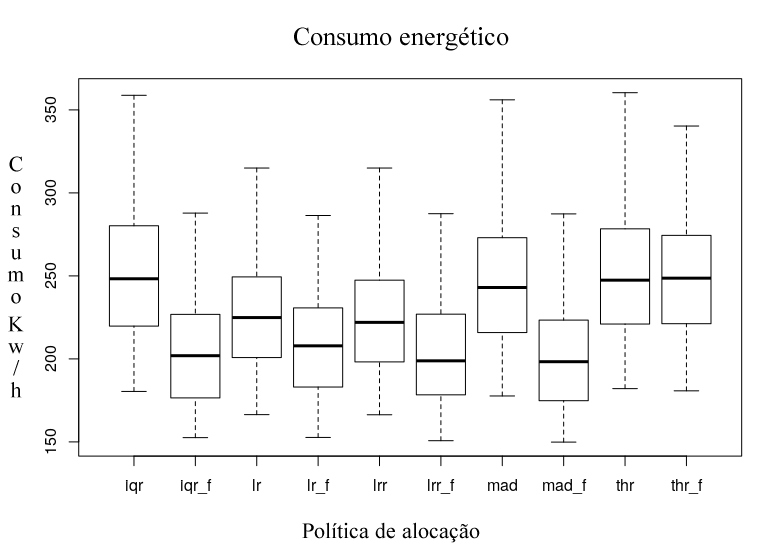
\includegraphics[scale=0.55]{images/resultados/energia_geral_pt.png} %0.44
\caption{Consumo energético}
\label{fig:avaliacao_energetica}
\end{figure}

É possível observar a economia de energia em relação aos outros algoritmos:  para a política IQR\_fuzzy em comparação com a IQR clássica o ganho foi de 15.43\%, no caso da política LR\_fuzzy em comparação a LR clássica o ganho foi de 9.39\%, na MAD\_fuzzy comparada com a MAD clássica o ganho foi de 15.64\% e por fim na THR\_fuzzy comparada com a THR clássica o ganho foi de 0.7\%.

\newpage

A porcentagem do número de VMs que infringiram o SLA é apresentado na Figura~\ref{fig:sla_geral}, quanto menor o valor melhor é o resultado. 

\begin{figure}[h]
\centering
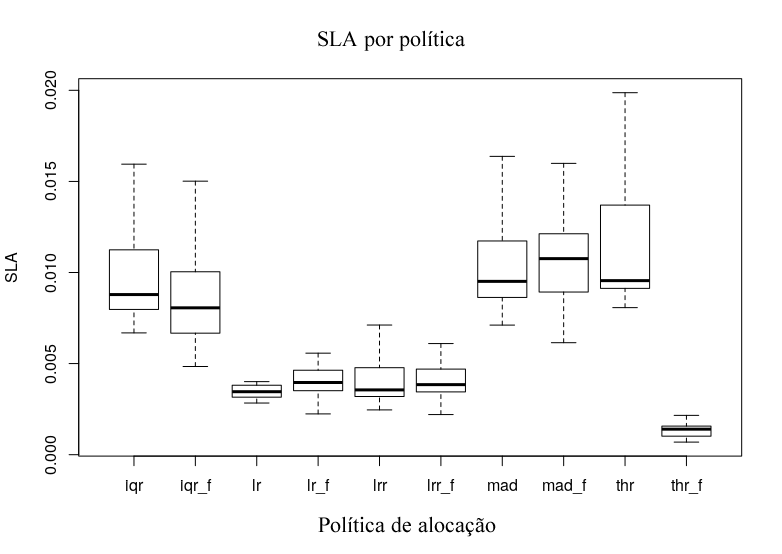
\includegraphics[scale=0.55]{images/resultados/geral_sla.png} %0.44
\caption{Violação de SLA por política}
\label{fig:sla_geral}
\end{figure}

No caso da política IQR\_fuzzy a média ficou 15.68\% mais baixa que o IRQ clássico, no LR\_fuzzy ficou 2.5\% maior que o LR clássico, no  LRR\_fuzzy ficou 4.76\% menor comparado com o LRR clássico, no MAD\_fuzzy ficou 0.93\% maior comparado com o MAD clássico e por fim no THR\_fuzzy ficou 88.8\% menor que o THR clássico.

O tempo médio que o SLA permaneceu sendo infringido é apresentado na Figura~\ref{fig:sla_tempo_host_ativo}, quanto menor o valor melhor é o resultado.


\begin{figure}[h]
\centering
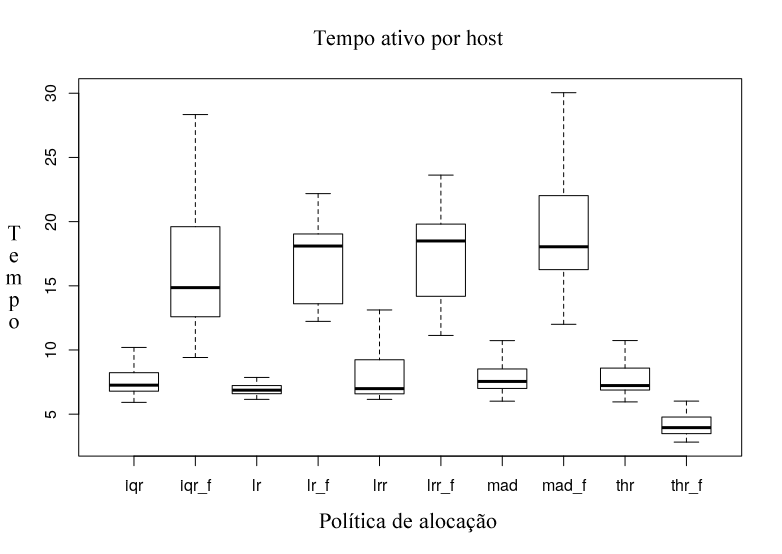
\includegraphics[scale=0.55]{images/resultados/sla_temp_por_host_ativo.png} %0.27 %0.44
\caption{Tempo médio de SLA infringido por host}
\label{fig:sla_tempo_host_ativo}
\end{figure}

No caso da política IQR\_fuzzy a média obtida foi 50.77\% maior que a IQR clássica, na LR\_fuzzy a média obtida foi 54.71\% maior que a LR clássica, na LRR\_fuzzy a média obtida foi 53.71\% maior comparado com a LRR clássica, na MAD\_fuzzy a média obtida foi 58.62\% maior comparado com a MAD clássica e, por fim, na THR\_fuzzy a média obtida foi 47.58\% menor que o THR clássico.

%A quantidade de MVs migradas é apresentada na Figura~\ref{fig:vm_migradas}, quanto menor o valor melhor é o resultado. No caso da política IQR\_fuzzy obteve uma diminuição de 49.36\% comparada com a IQR clássica, na LR\_fuzzy obteve uma diminuição de 41.67\% comparada com a LR clássica, na MAD\_fuzzy obteve uma diminuição de 51.56\% comparada com a MAD clássica, e por fim, a THR\_fuzzy teve a melhora mais expressiva, tendo uma diminuição de 71.95\% comparada com a THR clássica.

A quantidade de MVs migradas é apresentada na Figura~\ref{fig:vm_migradas}, quanto menor o valor melhor é o resultado. 

\begin{figure}[h]
\centering
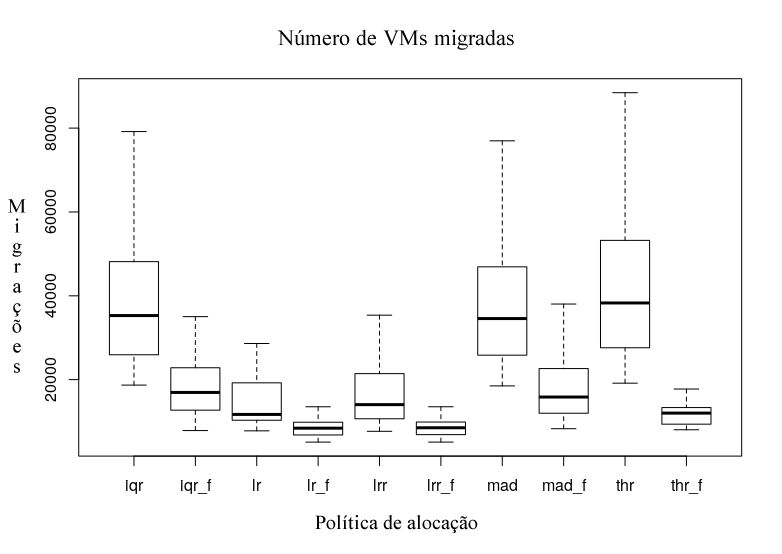
\includegraphics[scale=0.55]{images/resultados/vms_migradas.png} %0.44
\caption{VMs migradas}
\label{fig:vm_migradas}
\end{figure}

Foram obtidos os valores de 49.36\%, 41.67\%, 51.56\% , 71.95\% , são respectivamente para a diferença da média de IQRF, LRF, LRRF, MADF e THRF obtendo menor número de MVs migradas comparado com suas respectivas abordagens que empregam a lógica clássica.

\newpage

A Degradação do SLA devido a migração de MVs é apresentada na Figura~\ref{fig:degradacao_sla_migracao}, quanto menor o valor melhor é o resultado.

\begin{figure}[h]
\centering
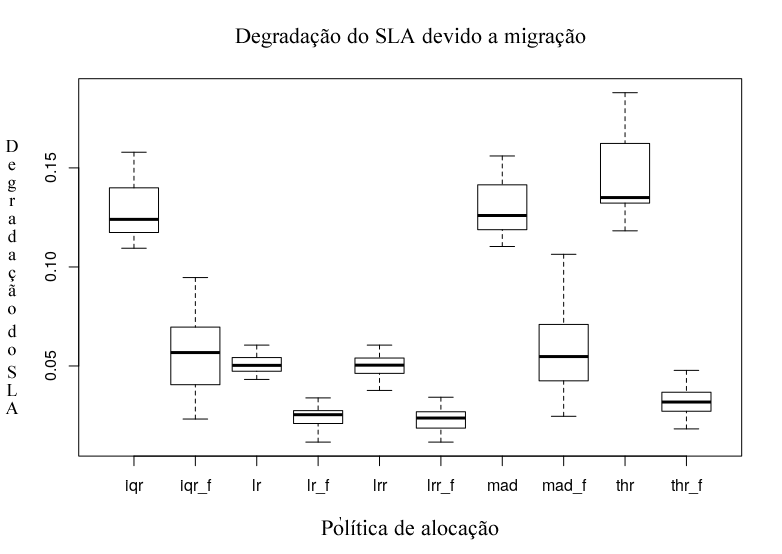
\includegraphics[scale=0.55]{images/resultados/degradacao_sla_devido_migracao.png} %0.45
\caption{Degradação do SLA devido a migração de MVs}
\label{fig:degradacao_sla_migracao}
\end{figure}

Foram obtidos os valores de 54.97\%, 52.26\%, 54.45\%, 55.18\% e 77.70\%, são respectivamente para a diferença da média de IQRF, LRF, LRRF, MADF e THRF obtendo menor degradação comparado com suas respectivas abordagens que empregam a lógica clássica.

\subsection{Estudo de caso 2}

Nesta seção, são apresentados os resultados obtidos com o emprego dos métodos das Ordens Admissíveis para ordenação da lista de intervalos obtida como saída do SBRF2, com intuito da detecção mais aproximada do nível de utilização dos hosts no ambiente de nuvem simulado.

\newpage

A avaliação do consumo de energia é apresentada através do boxplot da Figura ~\ref{fig:EvaEnergy}.

\begin{figure}[h]
\centering
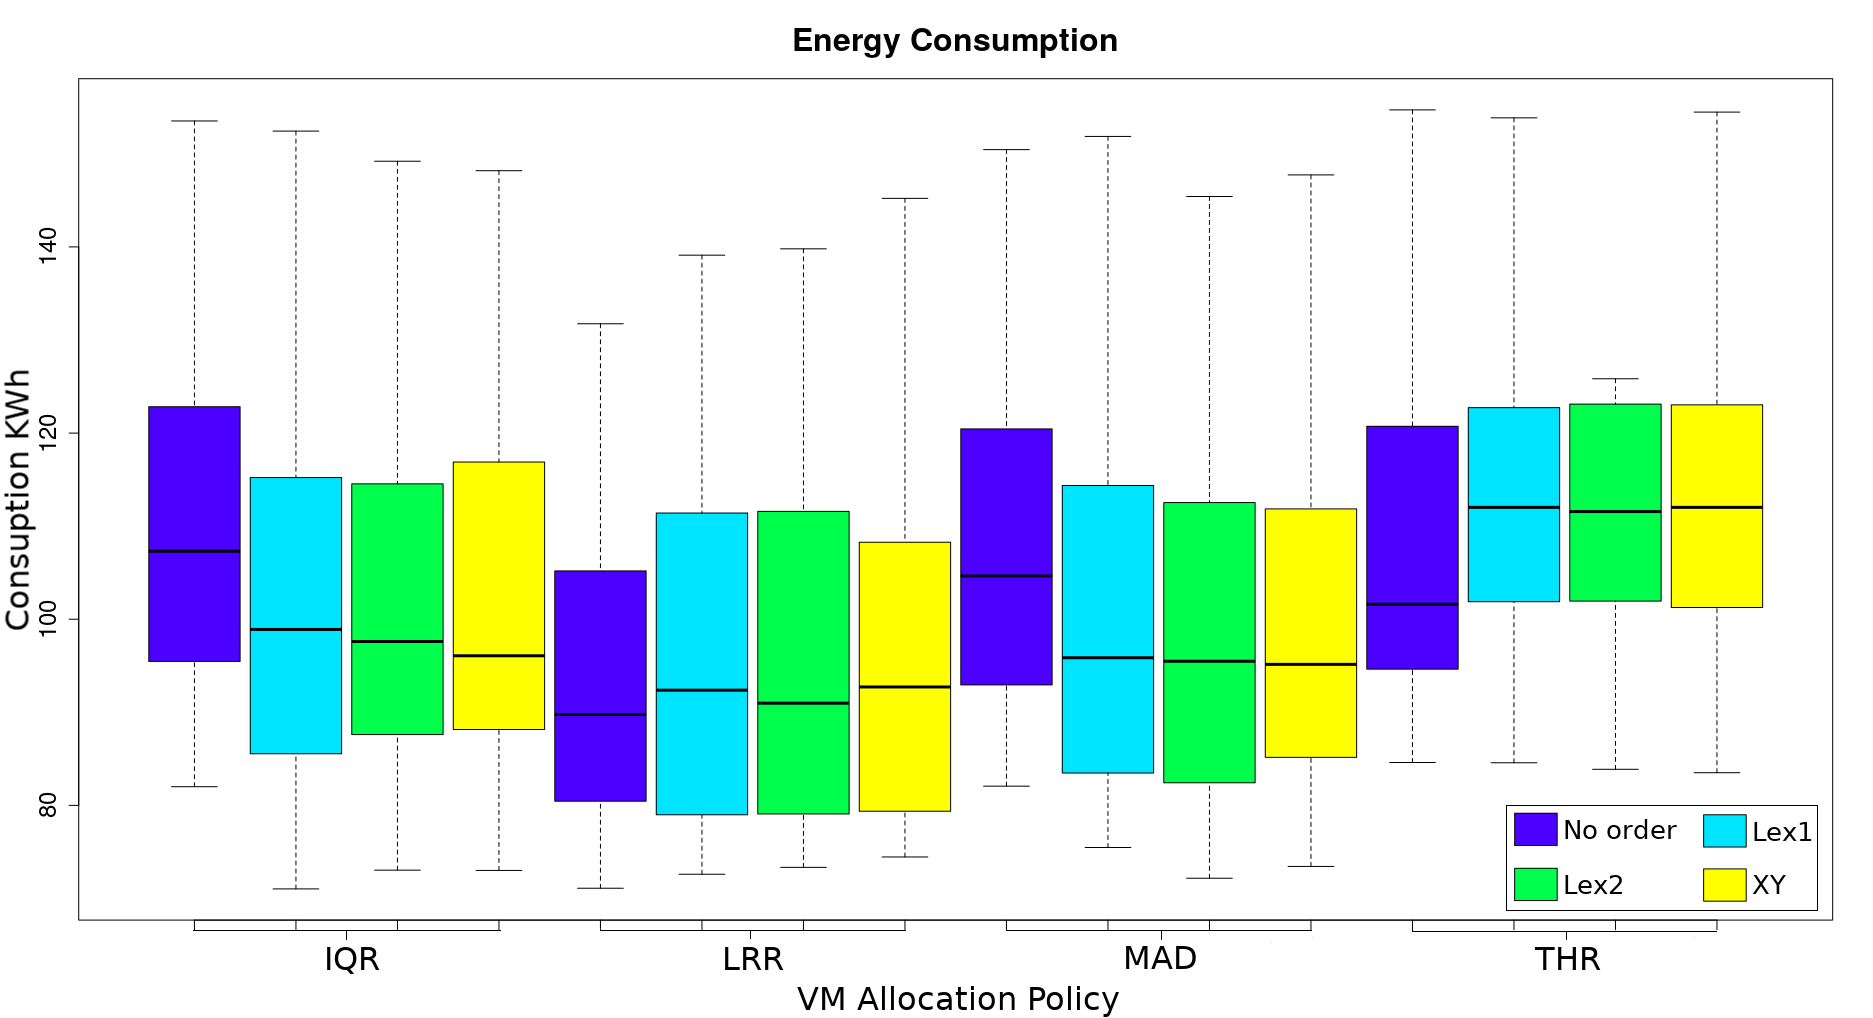
\includegraphics[scale=0.18]{images/energy5_fuzz_ieee_2019.png} %0.27
\caption{Consumo Energético}
\label{fig:EvaEnergy}
\end{figure}

Pode-se observar que a abordagem de seleção de host proposta com emprego das Ordens Admissíveis alcançou ganhos consideráveis em economia de energia, com a política IQR$\_$XY em relação ao IQR alcançou 8,83\% de ganho, no caso do MAD$\_$Lex2 em relação para MAD alcançou 8,72\%, em THR$\_$ XY comparado a THR 22,43\%.


O boxplot da Figura~\ref{fig:EvaSLA} apresenta resultados de SLA.

\begin{figure}[h]
\centering
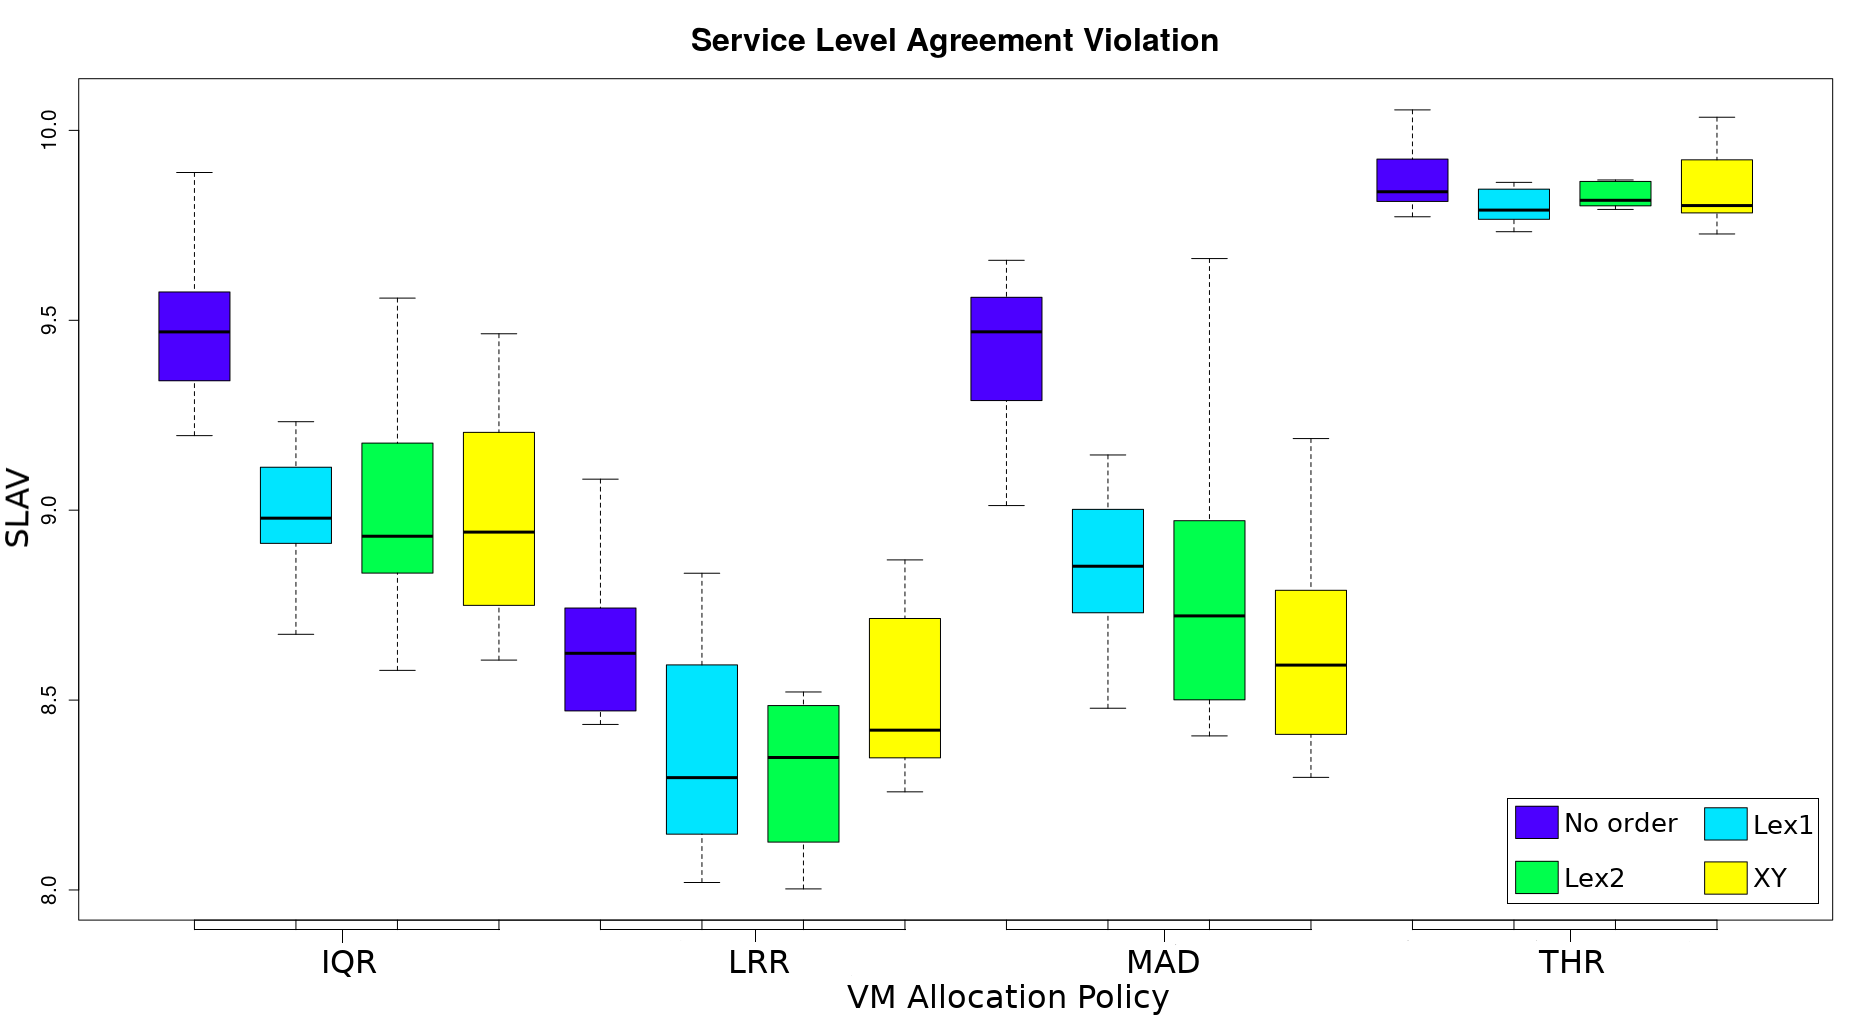
\includegraphics[scale=0.18]{images/slav4_fuzz_ieee_2019.png} %0.27
\caption{Média de Violação de SLA}
\label{fig:EvaSLA}
\end{figure}

A abordagem proposta alcançou resultados de 6.11\% com IQR$\_$XY comparado a IQR, para LRR$\_$ Lex2 4.02\% em relação a LRR, THR$\_$Lex1 25\% em oposição a THR e finalmente, MAD $\_$XY analisado a MAD obteve 9.06\%, correspondendo as melhores médias de violação de SLA.

\chapter{Conclusão} \label{capConclusao}

Neste trabalho, apresentamos o desenvolvimento do módulo fCloud: Sistema Fuzzy que seja capaz de tratar a incerteza do especialista em determinar a utilização de uma máquina física em um ambiente de CN usando Lógica Fuzzy Tipo-2 e Ordens Admissíveis como parte da consolidação das VMs. 

Foram simulados e comparados com o f-ClouD cinco algorimos conhecidos: Intervalo Interquartílico (\emph{Inter Quartile Range (IQR)}), Regressão Robusta Local (\emph{Local Robust Regression (LRR)}), Desvio Absoluto Mediano (\emph{Median Absolute Deviation (MAD)}) e Limite estático (\emph{Static Threshold (THR)}). 

Em cada execução, a política de seleção de VMs usada foi a Seleção aleatória (\emph{Random Selection (RS)}). 

Todos os algoritmos escolhidos tratam as incertezas presentes no ambiente usando uma abordagem clássica. No f-ClouD, a abordagem  mostra o potencial da lógica fuzzy, conquistando ganhos consideráveis em especial na eficiência energética, atingindo ganhos de 15.64, 15.43 e 9.19\% em relação a MAD, IRQ e LR respectivamente. 

Também houve um ganho expressivo no caso do tempo médio que o SLA permaneceu sendo infringido, no caso do algoritmo THR o ganho foi de 47.58\%.

No caso da abordagem que explorava uso de ordens admissíveis, na maioria dos casos obteve-se bons resultados em relação a eficiência energética, alcançando ganhos de 8.83\%, 22.43\% em relação aos algoritmos clássicos IRQ e MAD, usando ordens de Xu e Yager. Também houve um ganho expressivo considerando o SLA, com ganhos de 9.06\% no caso do MAD com ordem de Xu e Yager e de 25\% na THR utilizando ordem Lex1.

Os trabalhos futuros buscam otimizações no f-ClouD no sentido de novas políticas de alocação de MVs. No uso de fundamentação baseada em LF, considera-se o uso de múltiplos especialistas com suporte na análise de medidas de consenso para conciliação de opiniões. 



%In most cases, the proposed approach using Type-2 Fuzzy Logic obtained good results about energy efficiency, reaching gains of 8.83, 22.43\% to IRQ, MAD and LRR lost 4.19\% with using orders, Xu and Yager. Considering the SLA, the gains were 9.06\% of MAD with the order of Xu and Yager and 25\% with THR applying the ordering of Lex1


% Bibliografia http://liinwww.ira.uka.de/bibliography/index.html um
% site que cataloga no formato bibtex a bibliografia em computacao
% \bibliography{nomedoarquivo.bib} (sem extensao)
% \bibliographystyle{formato.bst} (sem extensao)

\bibliography{bibliografia} 
\bibliographystyle{abnt}
%\bibliographystyle{plain}


\end{document}

\begin{comment}

Backup Introdução
Com o sucesso da internet surgiram diversos desafios para as empresas que prestam serviços de TI(Tecnologia da informação) para a população, softwares necessitam cada vez mais de computação trazendo um maior custo para elas pois assim é necessário um alto investimento em equipamentos e ainda há a questão do alto consumo energético.

De acordo com o relatório do Conselho de Defesa dos Recursos Naturais NRDC\footnote{https://www.nrdc.org/} dos Estados Unidos EUA, em 2014, somente os data centers nos EUA consumiram uma estimativa de 70 bilhões de quilowatts/hora kWh, representando cerca de 1,8\% do consumo total de eletricidade dos EUA \cite{shehabi2016united}.

A busca por eficiência energética sem perda de desempenho fez com que diversos conceitos fossem criados, entre um deles se destaca a Computação em Nuvem, que consiste em uma distribuição dos serviços de computação (alocação de servidores, armazenamento, banco de dados, etc) em que não há a necessidade de o usuário ter um grande investimento comprando equipamentos e ainda ele só irá pagar por o que for usado.

Contudo, os principais desafios da CN são: provisionamento automático de serviço, migração de MVs, consolidação de servidores, gerenciamento de energia e segurança de dados. Neste trabalho a área a ser abrangida é a de migração de VMs, onde será proposto um algoritmo que procura uma melhor utilização dos servidores físicos do ambiente de CN mantendo um padrão de qualidade satisfatório para o usuário final.
\end{comment}

